% !TeX encoding = UTF-8

% 载入 SJTUThesis 模版
\documentclass[type=bachelor,language=english]{sjtuthesis}
% 选项
%   type=[doctor|master|bachelor|course],     % 可选(默认:doctor),论文类型
%   zihao=[-4|5],                             % 可选(研究生默认:-4,本科默认:5),正文字号大小
%   language=[chinese|english],               % 可选(默认:chinese),论文的主要语言
%   review,                                   % 可选(默认:关闭),盲审模式
%   [twoside|oneside]                         % 可选(默认:twoside),单双页模式

% 论文基本配置,加载宏包等全局配置
% !TEX root = ./main.tex

\sjtusetup{
  %
  %******************************
  % 注意:
  %   1. 配置里面不要出现空行
  %   2. 不需要的配置信息可以删除
  %******************************
  %
  % 信息录入
  %
  info = {%
    %
    % 标题
    %
    title           = {RISC-V处理器微架构的设计与优化},
    title*          = {RISC-V SoC Design and Optimization},
    %
    % 标题页标题
    %   可使用“\\”命令手动控制换行
    %
    % display-title   = {上海交通大学学位论文\\ \LaTeX{} 模板示例文档},
    % display-title*  = {A Sample Document \\ for \LaTeX-based SJTU Thesis Template},
    %
    % 页眉标题
    %
    % running-title   = {示例文档},
    % running-title*  = {Sample Document},
    %
    % 关键词
    %
    keywords        = {计算机体系结构, 系统级芯片, 嵌入式系统},
    keywords*       = {Computer architecture, System on-chip, Embedded system},
    %
    % 姓名
    %
    author          = {史\quad{}历},
    author*         = {Li Shi},
    %
    % 指导教师
    %
    supervisor      = {钱炜慷},
    supervisor*     = {Prof. Weikang Qian},
    %
    % 副指导教师
    %
    % assisupervisor  = {某某教授},
    % assisupervisor* = {Prof. Uom Uom},
    %
    % 学号
    %
    id              = {517370910032},
    %
    % 学位
    %   本科生不需要填写
    %
    degree          = {工学学士},
    degree*         = {Bachelor of Science in Engineering},
    %
    % 专业
    %
    major           = {电子与计算机工程},
    major*          = {Electrical and Computer Engineering},
    %
    % 所属院系
    %
    department      = {密西根学院},
    department*     = {UM-SJTU Joint Institute},
    %
    % 课程名称
    %   仅课程论文适用
    %
    course          = {VE 450},
    %
    % 答辩日期
    %   使用 ISO 格式 (yyyy-mm-dd);默认为当前时间
    %
    % date            = {2014-12-17},
    %
    % 资助基金
    %
    % fund  = {
    %           {国家 973 项目 (No. 2025CB000000)},
    %           {国家自然科学基金 (No. 81120250000)},
    %         },
    % fund* = {
    %           {National Basic Research Program of China (Grant No. 2025CB000000)},
    %           {National Natural Science Foundation of China (Grant No. 81120250000)},
    %         },
  },
  %
  % 风格设置
  %
  style = {%
    %
    % 本科论文页眉 logo 颜色 (red/blue/black)
    %
    header-logo-color = red,
    title-logo-color = blue,
  },
  %
  % 名称设置
  %
  name = {
    % bib               = {References},
    % acknowledgements  = {谢\hspace{\ccwd}辞},
    % publications      = {攻读学位期间完成的论文},
  },
}

% 使用 BibLaTeX 处理参考文献
%   biblatex-gb7714-2015 常用选项
%     gbnamefmt=lowercase     姓名大小写由输入信息确定
%     gbpub=false             禁用出版信息缺失处理
\usepackage[backend=biber,style=gb7714-2015]{biblatex}
% 文献表字体
% \renewcommand{\bibfont}{\zihao{-5}}
% 文献表条目间的间距
\setlength{\bibitemsep}{0pt}
% 导入参考文献数据库
\addbibresource{bibdata/thesis.bib}

% 定义图片文件目录与扩展名
\graphicspath{{figures/}}
\DeclareGraphicsExtensions{.pdf,.eps,.png,.jpg,.jpeg}

% 确定浮动对象的位置,可以使用[H],强制将浮动对象放到这里(可能效果很差)
% \usepackage{float}

% 固定宽度的表格
% \usepackage{tabularx}

% 表格中支持跨行
\usepackage{multirow}

% 表格中数字按小数点对齐
\usepackage{dcolumn}
\newcolumntype{d}[1]{D{.}{.}{#1}}

% 使用长表格
\usepackage{longtable}

% 附带脚注的表格
\usepackage{threeparttable}

% 附带脚注的长表格
\usepackage{threeparttablex}

% 算法环境宏包
\usepackage[ruled,vlined,linesnumbered]{algorithm2e}
% \usepackage{algorithm, algorithmicx, algpseudocode}

% 代码环境宏包
\usepackage{listings}
\lstnewenvironment{codeblock}[1][]%
  {\lstset{style=lstStyleCode,#1}}{}

% 物理科学和技术中使用的数学符号,定义了 \qty 命令,与 siunitx 3.0 有冲突
% \usepackage{physics}

% 直立体数学符号
\newcommand{\dd}{\mathop{}\!\mathrm{d}}
\newcommand{\ee}{\mathrm{e}}
\newcommand{\ii}{\mathrm{i}}
\newcommand{\jj}{\mathrm{j}}

% 国际单位制宏包
\usepackage{siunitx}

% 定理环境宏包
\usepackage{ntheorem}
% \usepackage{amsthm}

% 绘图宏包
\usepackage{tikz}
\usetikzlibrary{shapes.geometric, arrows}

% 一些文档中用到的 logo
\usepackage{hologo}
\newcommand{\XeTeX}{\hologo{XeTeX}}
\newcommand{\BibLaTeX}{\textsc{Bib}\LaTeX}

% 借用 ltxdoc 里面的几个命令方便写文档
\DeclareRobustCommand\cs[1]{\texttt{\char`\\#1}}
\providecommand\pkg[1]{{\sffamily#1}}

% = = = = = = = = = = = = %
%     JI专用模板调整      %
% = = = = = = = = = = = = %
\usepackage{mwe}
\usepackage{blindtext}
\usepackage{titlesec}
\usepackage{setspace}

% Chapter
\renewcommand\chaptername{\relax}
% \titleformat{\chapter}[hang]{\normalfont\bfseries\LARGE\centering}{\thechapter\quad}{-6pt}{}
% \titlespacing{\chapter}{0pt}{*6}{*3}
% \titleclass{\chapter}{straight}

% Section
\titlespacing{\section}{0pt}{*4}{*1.5}
\titlespacing{\subsection}{0pt}{*4}{*1.5}
\titlespacing{\subsubsection}{0pt}{*4}{*1.5}

% Figure
\renewcommand{\figurename}{Illustration}

% Code
% \usepackage{minted}

% JI Citation formatting
\newcommand{\quickcite} [1] {(\parencite{#1}, \citeauthor{#1}, \citeyear{#1}: \citefield{#1}{pages})}

\newcommand{\quickcitenopage} [1] {(\parencite{#1}, \citeauthor{#1}, \citeyear{#1})}

\newcommand{\quickcitetwo}[2]{(\parencite{#1,#2}, \citeauthor{#1}, \citeyear{#1}: \citefield{#1}{pages}; \citeauthor{#2}, \citeyear{#2}: \citefield{#2}{pages})}

% 自定义命令

% E-mail
\newcommand{\email}[1]{\href{mailto:#1}{\texttt{#1}}}

% hyperref 宏包在最后调用
\usepackage{hyperref}


\begin{document}

%TC:ignore

% 标题页
\maketitle

% 原创性声明及使用授权书
\copyrightpage[scans/ji-copyright.pdf]

% 前置部分
\frontmatter

% 摘要
% !TEX root = ../main.tex

\begin{abstract}
% = = = = = = = = = = = = = = = = = = = %
%               中文摘要                % 
% = = = = = = = = = = = = = = = = = = = %
{
在过去的几十年中,人们在不断研发更高性能的处理器。但是,由于物理及材料科学方面的限制,摩尔定律将在不久的将来达到瓶颈。这促使着工程师们在计算机体系结构领域进 行新的尝试,以此来突破瓶颈。近年来,随着系统级芯片(SoC)技术的发展和特定领域应用的需求,在特定领域进行架构设计与优化变得越来越普遍。例如,因为嵌入式系统中的人 工智能(AI)应用通常需要同时达到高性能、低功耗和低造价这三个要求,人工智能领域的嵌入式系统对现有的芯片体系提出了很大的挑战。在这个项目中,我们设计了一款基于 RISC-V 指令集的处理器。这款处理器支持四路超标量执行,并且具备指令动态规划能力。 我们同时对该处理器进行了众多优化。例如,我们添加了近似计算单元,用以提升特定领域的计算性能和能耗比。最终,我们将这款 SoC 与周边设备一同放入模拟软件中进行测试。周边设备包括:缓存,输入输出设备等。我们的处理器在性能、功耗和成本三方面达到了很好的平衡,并且在特定应用的嵌入式系统领域给用户提供了较好的体验。
}

\end{abstract}

% 1.5倍行距
{
\setstretch{1.5}
\setlength{\parindent}{0pt}
\setlength{\parskip}{1em}

\begin{abstract*}

% = = = = = = = = = = = = = = = = = = = %
%               英文摘要                % 
% = = = = = = = = = = = = = = = = = = = %
{
People have continuously pursued higher performance of processors in the past few decades. However, due to physical and material limitations, Moore's Law is reaching its boundary soon, forcing engineers to make new attempts in the field of computer architecture. Domain-specific architecture design and optimization is increasingly popular recently with emerging technology in systems on-chip (SoC) design as well as the need for domain-specific applications. One of the main challenges is raised from the domain of AI-oriented embedded systems, as AI applications in embedded systems usually require high performance, low power consumption and low cost at the same time. In this project, based on RISC-V instruction set architecture (ISA), we design a processor that supports 4-way superscalar execution and instruction dynamic scheduling. We apply further optimizations, e.g., approximate computing units, to enhance performance and energy efficiency for domain-specific applications. Finally, we set up the SoC and peripheral components including cache and I/O devices in software simulator tools. Our processor keeps a good performance-energy-cost balance and offers users good experience for specific applications in embedded systems.
}

\end{abstract*}

}

% 目录
\tableofcontents

%TC:endignore

% 主体部分
\mainmatter

% 正文内容
{
\setstretch{1.5}
\setlength{\parindent}{0pt}
\setlength{\parskip}{1em}

% = = = = = = = = = = = = = = = = = = = = = %
%                  Chapters                 %
% = = = = = = = = = = = = = = = = = = = = = %

% !TEX root = ../main.tex

% = = = = = = = = = = = = = = = = = = = %
%             Introduction              % 
% = = = = = = = = = = = = = = = = = = = %

\let\clearpage\relax
\chapter{Introduction}

During the past decade, people have tried to build machines with better computing performance. Frequency scaling was first used to enhance the performance of the system. Since clock frequency is the ``heart rate'' of a computer, frequency ramping has traditionally been the dominant force in the improvement of performance for commodity processors from the mid-1980s to about the end of 2004 \cite{frequency_ramping}.  However, increases in frequency also lead to increases in power consumption.  It was also because of the power wall that Intel canceled its Tejas and Jayhawk processors in 2004 \cite{intel}.

Fig.~\ref{frequency} illustrates the improvement in clock frequency over time, measured in megahertz (millions of cycles per second). Clearly, clock-frequency improvements have been stalled and limited to about 3-4GHz due to power consumption nowadays \cite{nap}.
\begin{figure}[!htp]
    \centering
    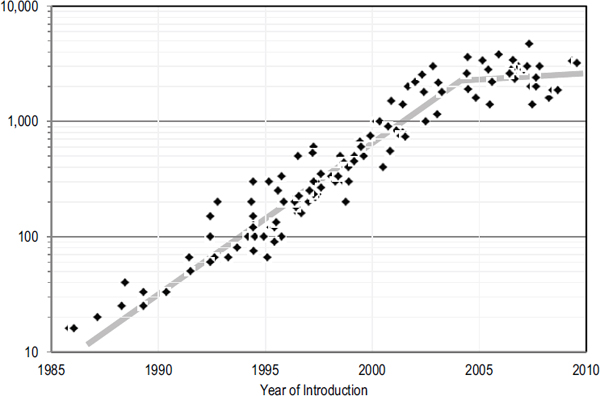
\includegraphics[width=0.8\linewidth]{figure/frequency.jpg}
    \caption{Microprocessor clock frequency (MHz) over time (1985-2010) \cite{nap}.}
    \label{frequency}
\end{figure}

In order to continuously improve the computing performance without depending on Moore's Law, people use parallel computing instead of sequential computing nowadays. What's more, products with parallel hardware and chip multi-processors has become one of the mainstream in the microprocessor industry \cite{nap}.

In addition to the parallel computing, people also leave the optimization of computer architecture as the future of computing. Domain-specific architecture design and optimization is one of these topics and it is really hot these days because of the need for AI and other applications. A groundbreaking example for domain-specific architecture is Google's tensor processing unit (TPU), which was first deployed in 2015 and now serves more than 1 billion people. Compared with contemporary CPUs and GPUs using similar technologies, it runs deep neural networks (DNN) 15 to 30 times faster and has 30 to 80 times better energy efficiency \cite{xxx}.

The biggest challenge in domain-specific architecture design was raised from the domain of the embedded system. These days embedded system start to adapt algorithms which need very large computing power. For example, Tesla's automotive car needs to process millions of pixels in short latency and feed them to the AI algorithm \cite{Tesla}.

Traditional AI computing platform like a CPU cannot provide so much computing power. Not only the computation limits the design, but energy efficiency is also vital for some system. A smart camera usually can be supplied limited1 energy. A camera on the drone, for example, must save energy to enlarge battery life. However, smart embedded systems do need complicated operations to implement neural networks, which usually costs lots of energy which is a dilemma. Finally, embedded systems are limited by cost. Generally, the engine controller under the hood of the car and the chip in the mobile phone needs to be below \$3-5 \cite{nap}. The chip in tennis shoes or greeting cards is even cheaper and cannot have a large chip area. Due to these reasons, some techniques like Single instruction, multiple threads (SIMT) may not be appropriate for such kind of system. Therefore, the need for an embedded system really calls for a novel design in computer architecture that can balance performance, energy efficiency, and cost for computation-intensive tasks.

There are some recent achievements in improving computer performance through optimizing of computer architecture. In a study applied in an application specific integrated circuit design (ASIC design), an high-accuracy approximate adder is introduced which can decrease the power and delay with a low relative error\cite{paper1}. Subsequently, a study introduces approximate operators into DNN hardware accelerators to reduce latency and energy consumption \cite{paper2}. Another study applies approximate divider and square root operations on their RISC-V design \cite{paper3}. But all these studies narrow their designs in some specific fields and the approximate adders and approximate operators actually can be used in a wide range of computing components including CPU, GPU and SoC. In this project, we propose an out-of-order processor design based on RISC-V with approximate computing units to reach a general solution for SoC design that can balance performance, energy and cost.

In this report, a short introduction and related works will be given in chapter 1 and 2. We will discuss our customer requirements and engineering specifications in chapter 3. Then the process of concept generation and selection will be discussed in details in chapter 4 and 5, followed by our final design of microarchitecture design and optimization in chapter 6. Implementation and validation will be discussed in chapter 7. Finally, our discussion, future work and conclusion of this project will be in chapter 8 and 9.

% = = = = = = = = = = = = = = = = = = = = = %
%              Related Work                 %
% = = = = = = = = = = = = = = = = = = = = = %

\let\clearpage\relax
\chapter{Related Work}

In the field of computer architecture, there exist several different processor design to speed up computing from different perspectives.

\section{MIPS Processor with Classical 5-stage Pipeline}
One popular design is MIPS processor with classical 5-stage pipeline. This architecture, proposed by Stanford University, uses MIPS Instruction Set Architecture (ISA) and five-stages pipeline, which enables the processor to execute more than one instruction in one clock cycle. However, all instructions in the processor are executed in-order with a single arithmetic logic unit (ALU) \cite{MIPS_V_Stage}. Therefore, the average Instruction per Cycle (IPC) is less than five, which is not efficient enough.

\section{Rocket Core}
Another widely-used architecture is Rocket Core, which is designed by UC Berkeley. Compared to classical 5-stage MIPS processor, Rocket Core has a Floating Point Unit (FPU) and a co-processor, called ``ROCC''. The specialized FPU speeds up the floating-point computing. Meanwhile, the co-processor enables users to customize their instructions \cite{Rocket_Core}.

\section{The Berkeley Out-of-Order Machine}\label{section: BOOM}
For further improvement, UC Berkeley releases an architecture for out-of-order execution, called ``BOOM''. This structure has up to 10 pipeline stages. What's more, instructions are executed out-of-order in this processor \cite{Boom}. Therefore, it is far more efficient than previous structures.

All architectures mentioned above do not have accelerator for machine learning or approximate computing. In comparison, our final product will have approximate computing unit in Execution stage to speed up machine learning. We believe that with these accelerators, our architecture will performance better in certain situations.

\section{Hummingbird E203}
Humming bird E203 is one of the most popular open-source RISC-V SoC among Chinese community and was designed by Zhenbo Hu's team in China \cite{E203}. It is designed for embedded systems with extremely low power consumption and circuit area, and is suitable for research purpose.


% = = = = = = = = = = = = = = = = = = = = = %
%              Specifications               %
% = = = = = = = = = = = = = = = = = = = = = %

\let\clearpage\relax
\chapter{Customer Requirements \& Engineering Specifications}

\section{Customer Requirements (CR)}
Since our project is experimental and research-oriented, there do not exist specific customers for our design. However, customer requirements are still necessary, as after the completion of our project, potential embedded system customers may be interested. Meanwhile, mainstream CPU and SoC evaluation indices still apply to our design, e.g., core frequency, performance, energy efficiency, power consumption, etc. Briefly speaking, our target market is artificial intelligence hardware systems, and the consumers include users who want to run machine learning applications in their embedded systems.

We divide our customer requirements into three categories: general (G), performance (P), and embedded system (ES). For the general part, customers may require that the design should be compatible to general RISC-V applications, and attached with clear documentations. Target users of our design may include computer science researchers, embedded system users, or both. The former requires the performance part, e.g., good performance for machine learning applications, and the latter requires the embedded system part, e.g., low power consumption and quick response.


\subsection{General Requirements}
The main concern for the general requirements part is to set up proper constraints so that we can achieve good compatibility as well as usability. This is determined by the characteristics of our target market and consumers.

The target market of our SoC is a sub-division of the traditional computing hardware market, which requires tight constraint on performance, cost and energy efficiency. Thus, the general requirement should be a super-set of current computing market. For example, microprocessors and computing system based RISC-V ISA has solid ecosystem and active community. Tool chains like \texttt{gcc} compiler support, Linux kernel support and verification support are well established \cite{rvsoftware}. The market will welcome a new SoC which is fully compatible with current RISC-V ecosystem because the cost to adopt our product will be low and they will need fewer labors and less time, comparing to the product needs software part from scratch. Also, the competitive computing market requires good usability to win the business. The computing hardware market requires good documentations, as experienced engineers in this high standardized industry can be much more productive when the documentation follows professional protocols. This requirement can also be justified if we consider who is our target consumers. It is hard for startups or small size company to use our product because these companies generally cannot take the risk to adopt a new SoC. Our target consumer will be medium or large size, system level companies who want to use our SoC to increase their current product's efficiency. These companies have strong low-level research and development capability, and their software or application may be architectural specific. Therefore, they will prefer a new SoC with minimum architectural change and requires little effort to deploy their applications. Compatibility and usability are therefore the main points in the General requirements part.

As our SoC is based on the RISC-V architecture, being compatible with the RISC-V architecture is the most important constraint to consider. RISC-V is a family of ISA, so selecting a proper RISC-V ISA subset is critical. RISC-V ISA includes a base integer ISA, like RISC-V 32I, and optional extension to the base ISA. We want our SoC to be a stable target for RISC-V applications so that the application source code written in high level language like C/C++ can be correctly mapped to our SoC. To run general RISC-V applications, a RISC-V 32G is a reasonable target as suggested by the RISC-V specification \cite{RISC-V_unprivileged_ISA}, which includes:
\begin{enumerate}
    \item RISC-V 32I base ISA
    \item RISC-V M extension, for integer multiplication and division
    \item RISC-V A extension, for atomic instructions
    \item RISC-V F extension, for single-precision floating-point
    \item RISC-V D extension, for double-precision floating point
\end{enumerate}

RISC-V 32G applications encode their instructions in 32 bits. However, due to the limited memory size of many embedded systems, we hope that the size of applications can be as small as possible. One of the solutions is to introduce RISC-V C extension for compressed instructions, where instructions are encoded in 16 bits. If time permits, we should add the support for RISC-V C extension to further optimize for embedded systems.

To enhance the usability of our SoC, a clear and clean documentation is needed. Enough documentation should be written for each module, each subsystem and the overall design. If time permits, some performance analysis can also be added in the documentation so the consumers can better unleash the potential of our SoC.

Finally, due to the requirement of cost control in most embedded system designs, our SoC should be as inexpensive as possible.

\textbf{General Requirements:}
\begin{enumerate}
    \item Is compatible with RISC-V applications (weight: 10)
    \item Has good documentation for reference (weight: 6)
    \item Is inexpensive (weight: 5)
\end{enumerate}


\subsection{Performance Requirements}
While Gordon Moore predicted the growth in semiconductor, he also foresaw its end 50 years later. In recent days, even the company uses Moore's law as a guideline have to slow their pace to build even smaller transistor. Therefore, our SoC faces a market which require smart design to achieve higher performance under current technology node.
The market will first need high performance for normal arithmetic operations. Although nowadays specific AI algorithms rely heavily on the matrix operations, the normal arithmetic operations still take great part in a program to do branching, jumping, indexing, etc. Thus, to achieve an overall high performance, we need to have high performance normal arithmetic units and designs so that this part will not be a bottleneck. For the normal operations, the performance throughput equals to frequency times the Instructions executed per clock cycle (IPC). In order to achieve a high throughput, we need both a high frequency and a high IPC. Designing more pipeline stages may help achieve higher clock frequency, but may result in higher plenty when there is a miss prediction. Dynamic scheduling is a technique to increase the throughput by enabling Out-of-Order execution when instructions have no dependency. This method extract instruction level parallelism and it is always combined with other technique like renaming, speculative execution to  maximize the outcome. Also, enough number of function unit is needed so that the pipeline will not stall during the congestion at the execution stage. Our SoC should adopt these traditional techniques to have a high performance on the traditional normal arithmetic operations.

The AI application is a hot topic today. The performance for running AI application is also demanded by our target market. One of the most significant properties of this application is that it is error torrent. During the inference, minor error will not introduce much difference on the final result. During the training, some error may even manually be introduced to increase the robustness of the algorithm. This makes approximate computing a potential way to achieve higher frequency by using circuits with fewer elements.

Another property of AI application is that it is data driven, which means it is usually memory-bounded. Our SoC needs a high performance memory subsystem to make sure the pipeline for AI application will not hungry for data and halt. By using memory hierarchy and introducing cache, we can exploit the temporary locality and spacial locality of memory access to increase the memory subsystem's performance. One of the most important parameter that determines the cache's performance is its size. A trade off between the cache size and other parameter like frequency needs to be made so that the overall performance can be improved.

Before our design is fixed, we want do some architecture exploration. Therefore, we want the parameters of some of the critical modules, like the reorder buffer size and cache size is configurable so that we can change them to evaluate performance.

\textbf{Performance Requirements:}
\begin{enumerate}
    \item Runs fast for normal arithmetic operations (weight: 8)
    \item Runs fast for machine learning applications (weight: 9)
    \item Runs fast for memory-bound applications (weight: 7)
    \item Can be configured with different parameters (weight: 2) % this should not be a ES requirement as it happens before design was fixed.
\end{enumerate}


\subsection{Embedded System Requirements}
Although the ware-house scale computing center still take plenty of the computation nowadays, the market has a trend to offload part of the computation to the edge because of security issue, latency issue, etc. Our SoC will be more competitive at the edge as the concept AI on things has attracted lots of attention. Therefore, we require our SoC satisfy some requirement for embedded system.

The embedded system is often energy-bounded as the power source is usually a battery. High power consumption is not allow because these scenario often require long battery life. The can be evaluated using the number of operations processed within unit energy, so our SoC should have a limited number at this part. Some embedded system also have requirement on latency. For AR/VR application, this requirement is necessary as longer latency will cause discomfort. We hope our SoC can provide a low average response time to a request for service. The market also requires embedded SoC have low cost, as the embedded system application is normally cost sensitivity. This can be evaluated by the usage of resources on the FPGA, like look-up tables (LUTs), block RAMs (BRAMs) and digital signal processors (DSPs). The embedded system also has to need to connect to various types of peripherals, so have more I/O controllers can make our product more competitive on the market.

\textbf{Embedded Requirements:}
\begin{enumerate}
    \item Saves power (weight: 6)
    \item Responds quickly (weight: 4)
    \item Low cost (weight: 3)
    \item Has good support for multiple I/O devices (weight: 3)
\end{enumerate}


\subsection{Benchmark Competitions against CR}
In this part, we quickly review some existing open-source solutions against customer requirements. This step gives us a better view of customer requirements as well as offers us some clue on how to design our own products based on existing solutions.

The evaluation is based on a 5-point scale, where 5 means ``satisfies perfectly'' and 1 means ``doesn't satisfy at all''. We select four open-source solutions to evaluate: MIPS processor with classical 5-stage pipeline, Rocket Core, Berkeley Out-of-Order Machine (BOOM), and Hummingbird E203. For instance, in terms of ``is compatible to general RISC-V applications'', we find that Rocket Core and BOOM have the best support, so we give them 5 points. Hummingbird E203 has limited support for RISC-V applications, so we give it 3 points. The MIPS processor with classical 5-stage pipeline is not compatible with RISC-V applications, so we give it 1 point.

The detailed benchmark competitions against CR are shown in the HOQ chart (Fig. \ref{qfd}).


\section{Engineering Specifications (ES)}
Based on the previous customer requirements, we come up with our engineering specifications of our project, which represent for the quantifiable measures to guide us to design the project properly that can meet customers' requirements. Table \ref{es} shows our overall engineering specifications in our project design.

\begin{table}[!htp]
\centering
\begin{tabular}{lcc}
\hline
\textbf{Engineering Specification} & \textbf{Unit} & \textbf{Target Value} \\
\hline
Support RV32G instruction set architecture (ISA) & -     & Yes          \\
Core frequency on FPGA test platform             & MHz   & 100          \\
Number of pipeline stages                        & -     & 9            \\
Instructions executed per clock cycle (IPC)      & -     & 0.5          \\
Support instruction dynamic scheduling           & -     & Yes          \\
Typical total cache size                         & KB    & 32           \\
Number of function units                         & -     & 6            \\
Average response time to a request for service   & ms    & 10           \\
Usage of look-up tables (LUT) on FPGA            & k     & 120          \\
Usage of block RAM (BRAM) on FPGA                & -     & 50           \\
Usage of digital signal processor (DSP) on FPGA  & -     & 30           \\
Power consumption on target FPGA test platform   & W     & 5            \\
Operations processed within unit energy.         & MOp/J & 25           \\
Number of flexibly-configured modules            & -     & 10           \\
Number of I/O device types                       & -     & 3            \\
User guide and programmers manual                & -     & Yes          \\
\hline
\end{tabular}
\caption{Engineering specifications.}
\label{es}
\end{table}

This should be a key step to ``translate'' customers' words into professional terms and specifications. For instance, when customers require that their RISC-V applications can run on our SoC, what we actually need is that our SoC should support RV32G ISA. In this part, we will explain how we check the cross correlation of ES, examine the benchmark competitions against ES, set our own target for ES, and most importantly, correlate CR to ES.


\subsection{Cross Correlation of ES}
In this step, we check the cross correlation of ES, and reveal some internal connection between each specification we just made in the previous step. For example, when we increase the number of function units, the usage of hardware resources also increases. When we want to support instruction dynamic scheduling to support out-of-order instruction execution, we can greatly improve the number of instructions executed per clock cycle, which is a significant mark of performance improvement.

This step also gives us a clear guidance on design trade-offs. The most evident contradiction is that the SoC we want to design can never achieve low cost, high performance, low power consumption at the same time, which exactly corresponds to our three different parts of customer requirements. For example, if we want to improve the performance, possible solutions include increasing the frequency, increasing the number of function units, etc., none of which is good for saving power and reducing cost.


The detailed cross correlation of ES is given in the HOQ chart (Fig. \ref{qfd}).


\subsection{Benchmark Competitions against ES \& Set Target for ES}
It is important to perform some benchmark on some existing solutions in terms of our engineering specifications, which enables us to understand better about drawbacks of existing solutions as well as our design targets in the future.

This process sometimes requires ``reverse engineering'' for commercial products, but should be much easier for open-source products. In our survey, except that Hummingbird E203 is partially open-source, all the other three processors are completely open-source, and we should be able to access the data conveniently. However, we need to pay attention that some data is still difficult to access, e.g., the average response time to a request for service. There are some reasons for this kind of lack of data. First, even though the processor design is open-source, the synthesis tool or the test suites are not open-source, leading to the difficulty to reproduce the test results. Second, even though the test processes are completely public, the results may depend on the specific hardware testing platform, which may be expensive or inaccessible. Third, some of the designs can be flexibly configured, and there is no standard or typical settings, as a result of which the test results under different settings can not be referred or compared directly.

In this step, we try our best to explore the data of these existing solutions. Some data can be easily accessed, e.g., the number of pipeline stages or whether instruction dynamic scheduling is supported, while some other data cannot. \cite{processor_benchmark} provides us with many useful indicators to evaluate a design and meanwhile gives us lots of data of both Rocket Core and BOOM, including usage of hardware resources, etc.

Based on the data of existing solutions, we come up with our target values for ES. For example, as our aim is to provide good experience for machine learning application users, performance is crucial to some applications like neutral network, and hence we decide to support instruction dynamic scheduling, and set a relatively high value of core frequency of our design. During the process of deciding our own targets, we mainly refer to the data of BOOM, but also look at the data of other three solutions.

The detailed benchmark competitions against ES and our targets for ES are shown in the HOQ chart (Fig. \ref{qfd}).

\subsection{Correlation from CR to ES}
In this step, we not only make our engineering specifications from scratch, but also check whether all the customer requirements can be covered in our specifications. While the following paragraphs give a short explanation on how we transform CR into ES.

\begin{enumerate}
    \item \textbf{General part}: As customers require that our SoC should be compatible to general RISC-V applications, we require that our SoC should support RV32G ISA. As customers need good and clear documentation, we require that we need to deliver SoC user guide and programmer manual. To control the cost, we need to control our circuit size by limiting our usage of hardware resources, e.g., usage of look-up tables (LUT), digital signal processors (DSP), and block RAMs (BRAM).
    \item \textbf{Performance part}: We want to optimize our SoC for three different customer scenarios: normal arithmetic operations, machine learning applications, and memory-bound applications. They share some common characteristics, e.g., they all require that our SoC should support instruction dynamic scheduling and as high core frequency as possible. Meanwhile, they differ in some specific aspects. For instance, as normal arithmetic applications and machine learning applications are mostly compute-bound, they will benefit more from the improvement on core frequency, instructions executed per clock cycle, and number of function units, while memory-bound applications will benefit more from the improvement on total cache size, as cache is used to accelerate the access to memory.
    \item \textbf{Embedded system part}: Customers require that our SoC works well in embedded systems. To save power, we need to monitor and control the power consumption and energy efficiency of our SoC. To achieve quick response, we need to measure the average response time to a request for service. To configure our SoC with different parameters easily, we need to increase the number of flexibly-configured modules in our digital design. To have good support for multiple I/O devices, we need to support multiple kinds of I/O types and test on various I/O devices.
\end{enumerate}

\section{Quality Function Development (QFD)}
We develop our House of Quality (HOQ) chart with QFD method. The HOQ chart is shown in Fig. \ref{qfd}.

\begin{figure}[!htp]
    \centering
    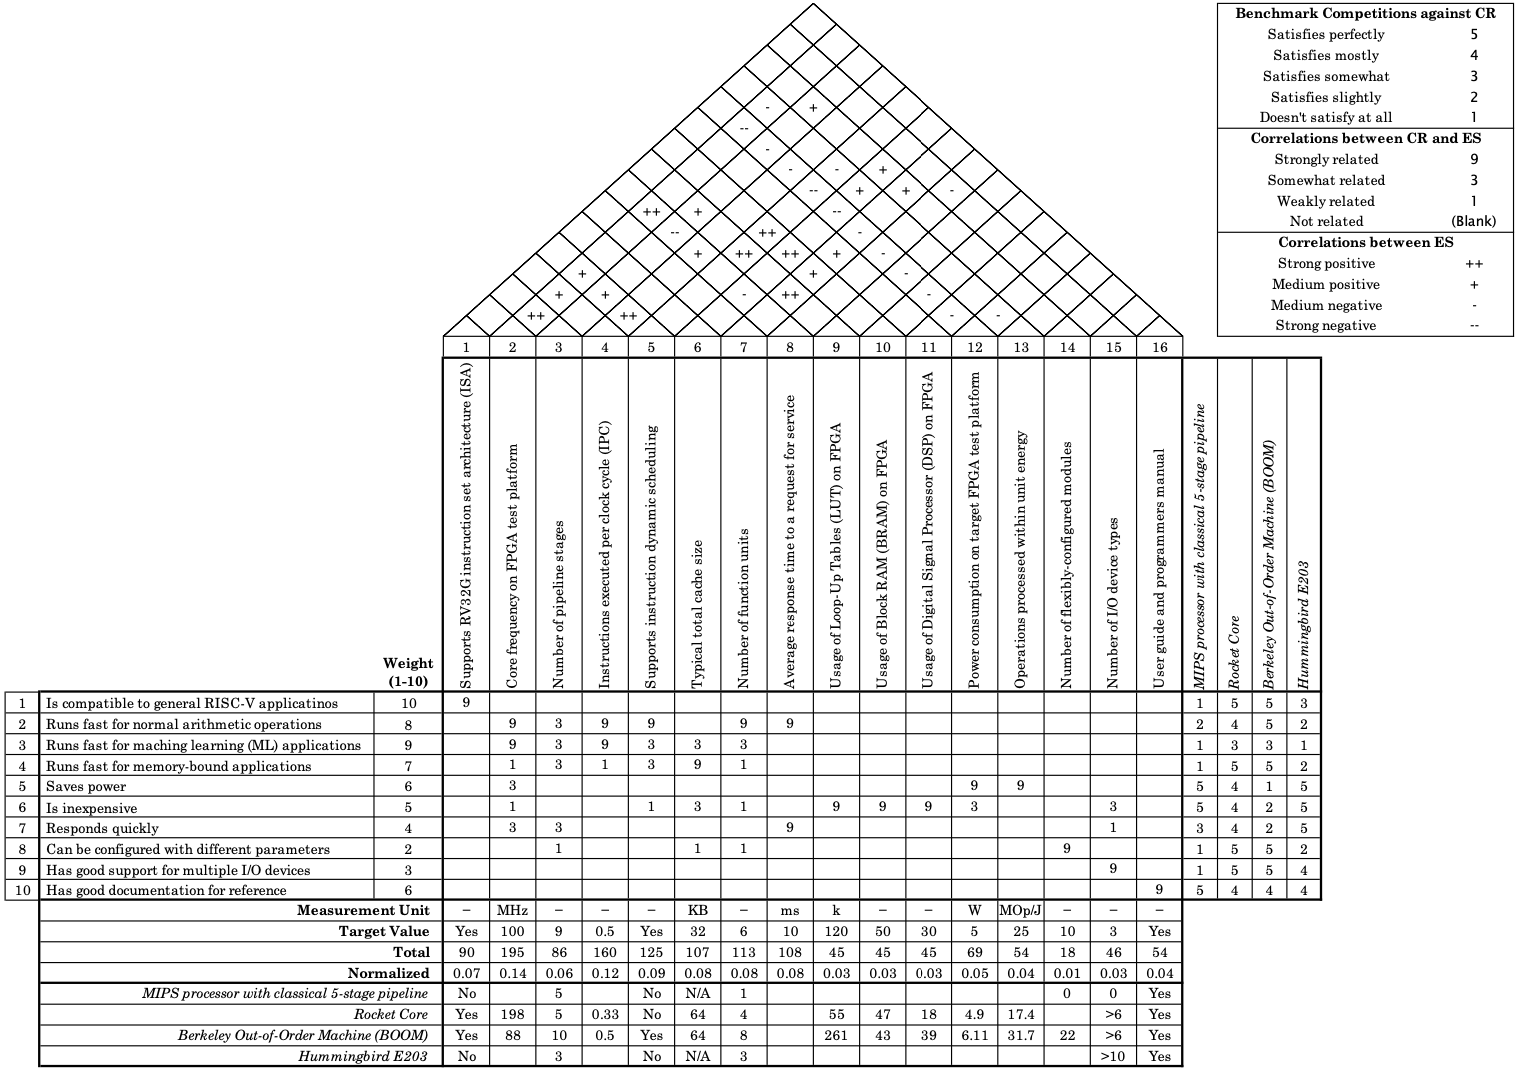
\includegraphics[width=\linewidth]{figure/qfd.png}
    \caption{House of Quality (HOQ) chart.}
    \label{qfd}
\end{figure}

The main steps of QFD method has been expanded in the previous sections. Finally we are able to examine our design priority according to ``Total'' and ``Normalized'' fields. The top 5 engineering specifications we need to consider are core frequency, instructions executed per clock cycle, support for instruction dynamic scheduling, number of function units, and average response time. The result generally matches our expectation that performance is still among the most important factors in embedded system SoC design. Meanwhile, some specifications like number of flexibly-configured modules are relatively not as important as previous ones.

% = = = = = = = = = = = = = = = = = = = = = %
%           Concept Generation              %
% = = = = = = = = = = = = = = = = = = = = = %

\let\clearpage\relax
\chapter{Concept Generation}

\section{ISA} %sj
An instruction set architecture (ISA) describes the capabilities of a processor. The ISA specifies how instructions should be formatted so that the control unit can correctly interpret them, and the meaning of those instructions in terms of their semantics.

Besides, an ISA also defines the supported data types, the registers, the hardware support for managing main memory, fundamental features and the input/output model of a processor. As such, an ISA represents an interface between programmer and an abstract processor rather than an exact specification of how the processor should be implemented \cite{Daniel}.

Therefore, to design our personal processor, we must choose an ISA that satisfies our design requirement. A good ISA can help us achieve our design specifications easily.

An ISA may be classified in a number of different ways. A common classification is by architectural complexity. A complex instruction set computer (CISC) has many specialized instructions, some of which may only be rarely used in practical programs. A reduced instruction set computer (RISC) simplifies the processor by efficiently implementing only the instructions that are frequently used in programs, while the less common operations are implemented as subroutines, having their resulting additional processor execution time offset by infrequent use \cite{risc_cisc}.

We will make our decision among all these ISAs.

\section{Microarchitecture} %sl
Comparing to ISA, which describes the overall architecture of a computer system that is usually visible to programmers, microarchitecture usually describes the way that how a specific processor design implements the ISA. Namely, to some extent the concepts of ISA and microarchitecure are orthogonal, i.e., one ISA can be implemented by many processors, while one microarchitecture can support different ISAs after necessary modifications. Unlike ISA, usually microarchitecture is invisible to programmers. For instance, in our out-of-order microarchitecture design, although the instructions are dynamically scheduled and executed, from the perspective of programmer, the instructions seem to be executed sequentially and follow the programmers' intention.

Therefore, a good microarchitecture design is key to a successful processor product. Even though different processors share the same ISA, they may differ in microarchitecture designed for different kind of market, e.g., high-performance computing or embedded systems.

In terms of the number of instructions that can be executed at the same time, we have scalar design and superscalar design. Fig.~\ref{fig:superscalar} demonstrates the difference between two kinds of design. While scalar design is able to execute one instruction at a time, superscalar design supports multiple channels to execute the instructions. Theoretically, for example, a 2-way superscalar design can double the performance. However, in reality, due to many external factors, e.g., data and control dependency, the speed-up ratio should be between 1 and 2.

\begin{figure}[!htp]
    \centering
    \begin{subfigure}{0.4\textwidth}
      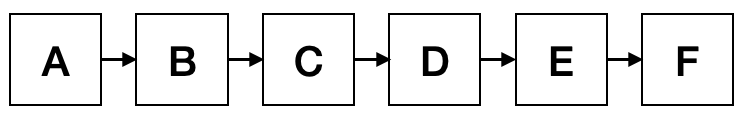
\includegraphics[width=\textwidth]{figure/scalar.png}
      \caption{Scalar execution.}
      \label{fig:superscalar-1}
  \end{subfigure}
  ~
  \begin{subfigure}{0.4\textwidth}
      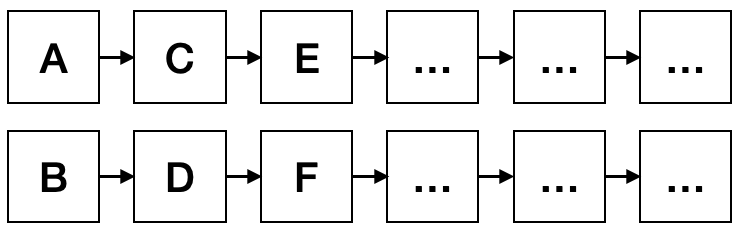
\includegraphics[width=\textwidth]{figure/superscalar.png}
      \caption{2-way superscalar execution.}
      \label{fig:superscalar-2}
  \end{subfigure}
  \caption{Scalar vs. superscalar processor design.}
  \label{fig:superscalar}
\end{figure}

In terms of instruction scheduling, we have in-order scheduling and out-of-order scheduling, or so-called instruction dynamic scheduling. Fig.~\ref{fig:o3} shows the differences between two ways of instruction scheduling mechanism. For example, instruction A requires 3 clock cycles to complete, but instruction B depends on the result of A. In the in-order design, B must wait until A is completed, but in the out-of-order design, we can execute instruction D (that is independent of A) prior to B, so that the performance is further improved. Most of modern processors for high-performance computing are based on out-of-order scheduling design.

\begin{figure}
    \centering
    \begin{subfigure}{0.4\textwidth}
        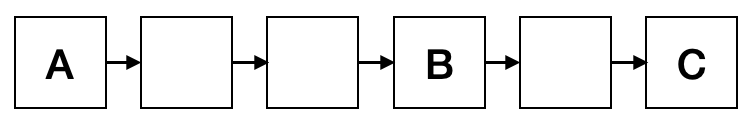
\includegraphics[width=\textwidth]{figure/in-order.png}
        \caption{In-order scheduling.}
        \label{fig:o3-1}
    \end{subfigure}
    ~
    \begin{subfigure}{0.4\textwidth}
        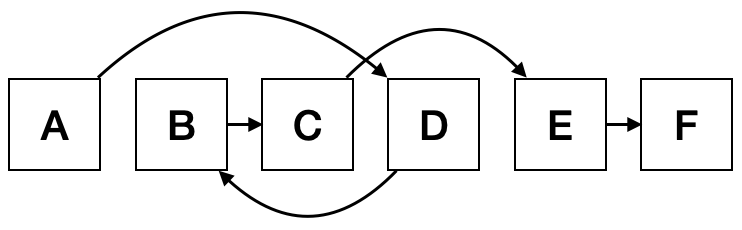
\includegraphics[width=\textwidth]{figure/out-of-order.png}
        \caption{Out-of-order scheduling.}
        \label{fig:o3-2}
    \end{subfigure}
    \caption{In-order vs. out-of-order instruction scheduling mechanism.}
    \label{fig:o3}
\end{figure}

\section{Verification \& SoC Integration} %yyc
% citation will be considered later
% citation: https://www.sciencedirect.com/topics/computer-science/design-verification

% citation: https://www.veripool.org/ftp/verilator_doc.pdf

% citation: https://github.com/riscv/riscv-isa-sim
\subsection{Verification}
The aim of verification is to make sure that the design meets the system requirements and specification. Normal approaches to verify design include following three ways [cite]:
\begin{enumerate}
    \item \textbf{Logic simulation}. The design is verified by performing a cycle accurate simulation. The detailed timing and functionality information can be check to see correctness.
    \item \textbf{Functional verification}. The design is checked against a functional models, which describe the correct behavior of the design. A behavior level simulation is performed to check the correctness of the design while timing detailed are ignored.
    \item \textbf{Formal verification}. This method includes property checking and equivalence checking.
\end{enumerate}

We emphasize on doing functional verification as well as logic simulation. We cannot perform formal verification because normally this requires commercial software support. Due to our budget constraints, we do not use this to check our model. For the logic simulation part, the verification process will be based on the logs and waveform, i.e., we check the logs and waveform to check our design's timing and behaviors. Although by logic simulation we can know whether our design is identical to our expectation, but they may not necessarily meet the RISC-V specification. We will use another verified RISC-V simulator as comparison to check the architectural correctness of our processor.

\subsection{SoC Integration}
A single CPU can do few things as it cannot perform IO. It can only run hardwired program from specific locations. Although we are using many tools to do the evaluation, this still make the whole development process inconvenient. We perform a SoC Integration aiming at providing our SoC IO capabilities, making it possible to dynamically loading program and output its computation result to the host machine. 

The SoC will integrate at least some memory devices. The whole simulation system will provide interface for the simulation host machine to communicate and verify the design under test.

% = = = = = = = = = = = = = = = = = = = = = %
%            Concept Selection              %
% = = = = = = = = = = = = = = = = = = = = = %

\let\clearpage\relax
\chapter{Concept Selection}

\section{ISA}\label{section:isa} %sj
There exist several popular instruction set architectures (ISAs), such as x86, MIPS, ARMv7 and RISC-V. As we mentioned before, they can be classified by their architectural complexity, e.g., memory addressing modes and instruction length. Since complex instruction set computer (CISC) ISAs are usually not open-source and too complicated for our project, we choose among reduced instruction set computer (RISC) ISAs. Following are three widely-used RISC ISAs.

\begin{enumerate}
\item \textbf{MIPS:} MIPS is a RISC ISA developed by MIPS Computer Systems. It is widely used in industry and also computer architecture courses for university students. Most of group members are familiar with MIPS Instructions and have development experience on it.

\begin{figure}[!htp]
    \centering
    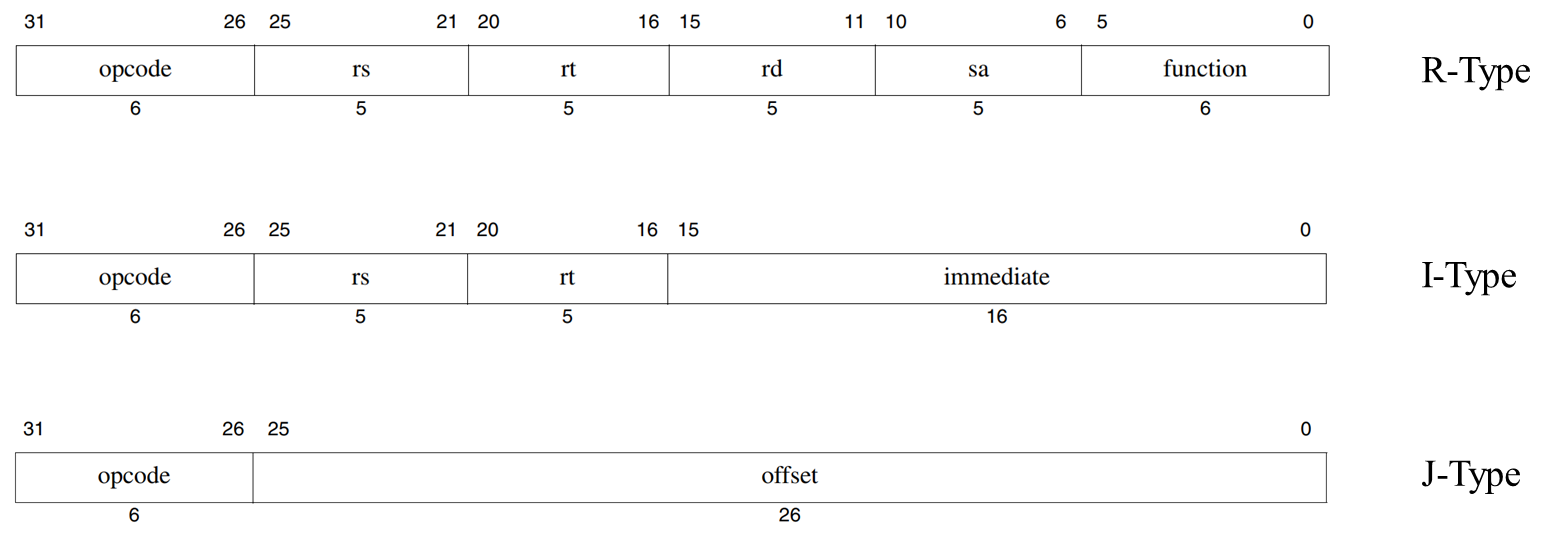
\includegraphics[width=0.7\textwidth]{figure/MIPS-instruction-format-18.png}
    \caption{MIPS instruction format\quickcitenopage{mips_ist}.}
    \label{fig:mips_inst}
\end{figure}

However, with many years of development, the design space of MIPS has been exploited, which will be an obstacle to further research. For example, originally branch delay slots are designed for reduce the cost of branch mis-prediction. However, it introduces unnecessary design complexity and does not always result in performance improvement.

\item \textbf{ARMv7:} ARM is a family of RISC ISA developed by Arm Ltd. Among them, ARMv7 is a classic structure applied in many areas. Due to its low cost, low power consumption, and low heat generation rate, ARMv7 is an ideal choice for light, portable, battery-powered devices, such as smartphones, Intenet of things (IoT) and other kinds of embedded systems.

\begin{figure}[!htp]
    \centering
    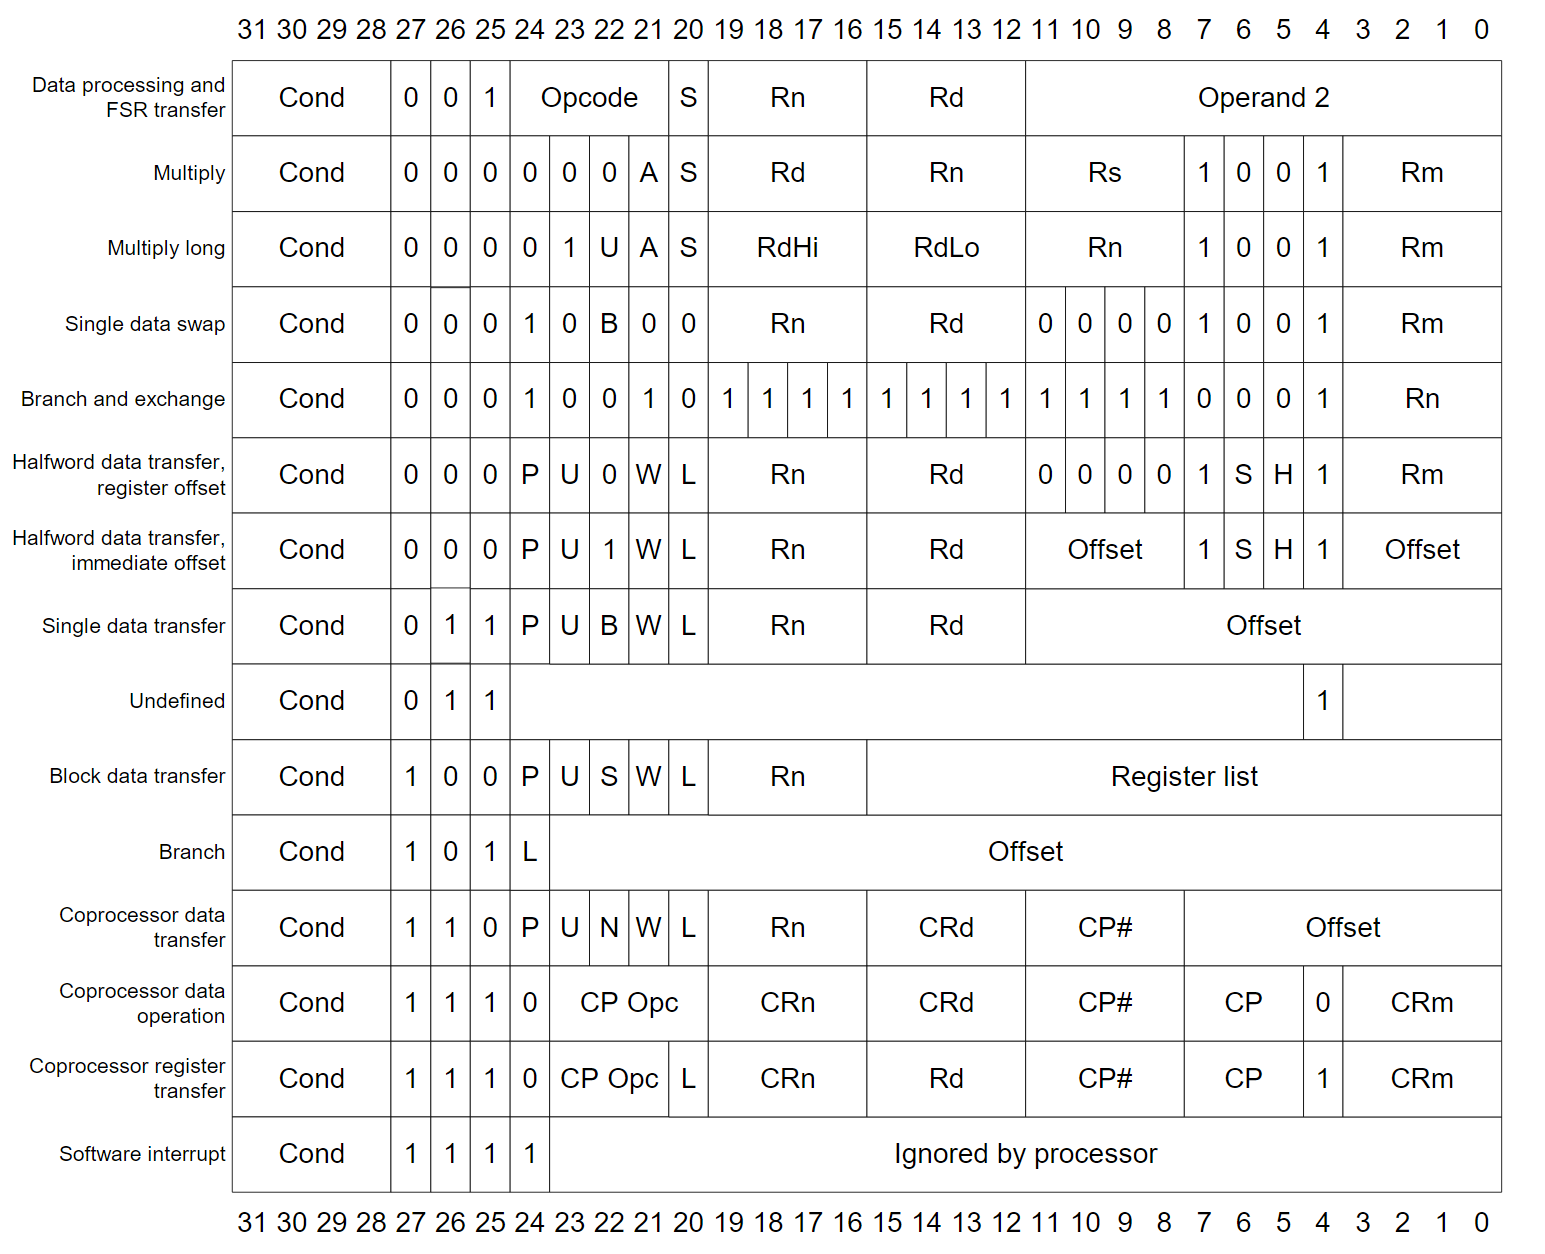
\includegraphics[width=0.85\textwidth]{figure/arm_ist.png}
    \caption{ARM instruction format\quickcitenopage{arm_ist}.}
    \label{fig:arm_ist}
\end{figure}

However, ARM does not allow users to custom their instructions without permission, i.e., we don't have design space to support our own customized instructions. Furthermore, to support more features, there are many advanced instructions and techniques in the ISA specifications, which means that it is difficult for us to implement in a short period.

\item \textbf{RISC-V:} RISC-V is an open standard RISC ISA. Unlike most other ISA designs, the RISC-V ISA is provided under open source license, i.e, it is completely free to use. Besides, RISC-V is also an emerging ISA during the past decade, which was initially introduced in 2010. It is simple but powerful for embedded system design. Therefore, it becomes our ideal ISA to implement in our processor design.

\begin{figure}[!htp]
    \centering
    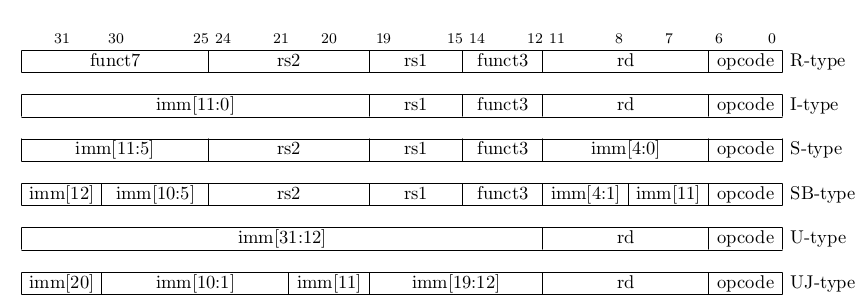
\includegraphics[width=0.85\textwidth]{figure/riscv-isa.png}
    \caption{RISC-V instruction format\quickcitenopage{RISC-V_unprivileged_ISA}.}
    \label{fig:RISCV_inst}
\end{figure}

However, compared to ARMv7 and MIPS, RISC-V supports fewer instructions, resulting in limited functions.

\end{enumerate}

\section{Microarchitecture} %sl
As mentioned in the previous section, microarchitecture determines the performance, power consumption and also cost of a processor and as a result is key to the success of a processor product. In this section, we use decision matrix to select our microarchitecture design based on customer requirements and engineering specifications. Illustration~\ref{fig:dm-uarch} shows the decision matrix of microarchitecture design.

\begin{figure}[!htp]
    \centering
    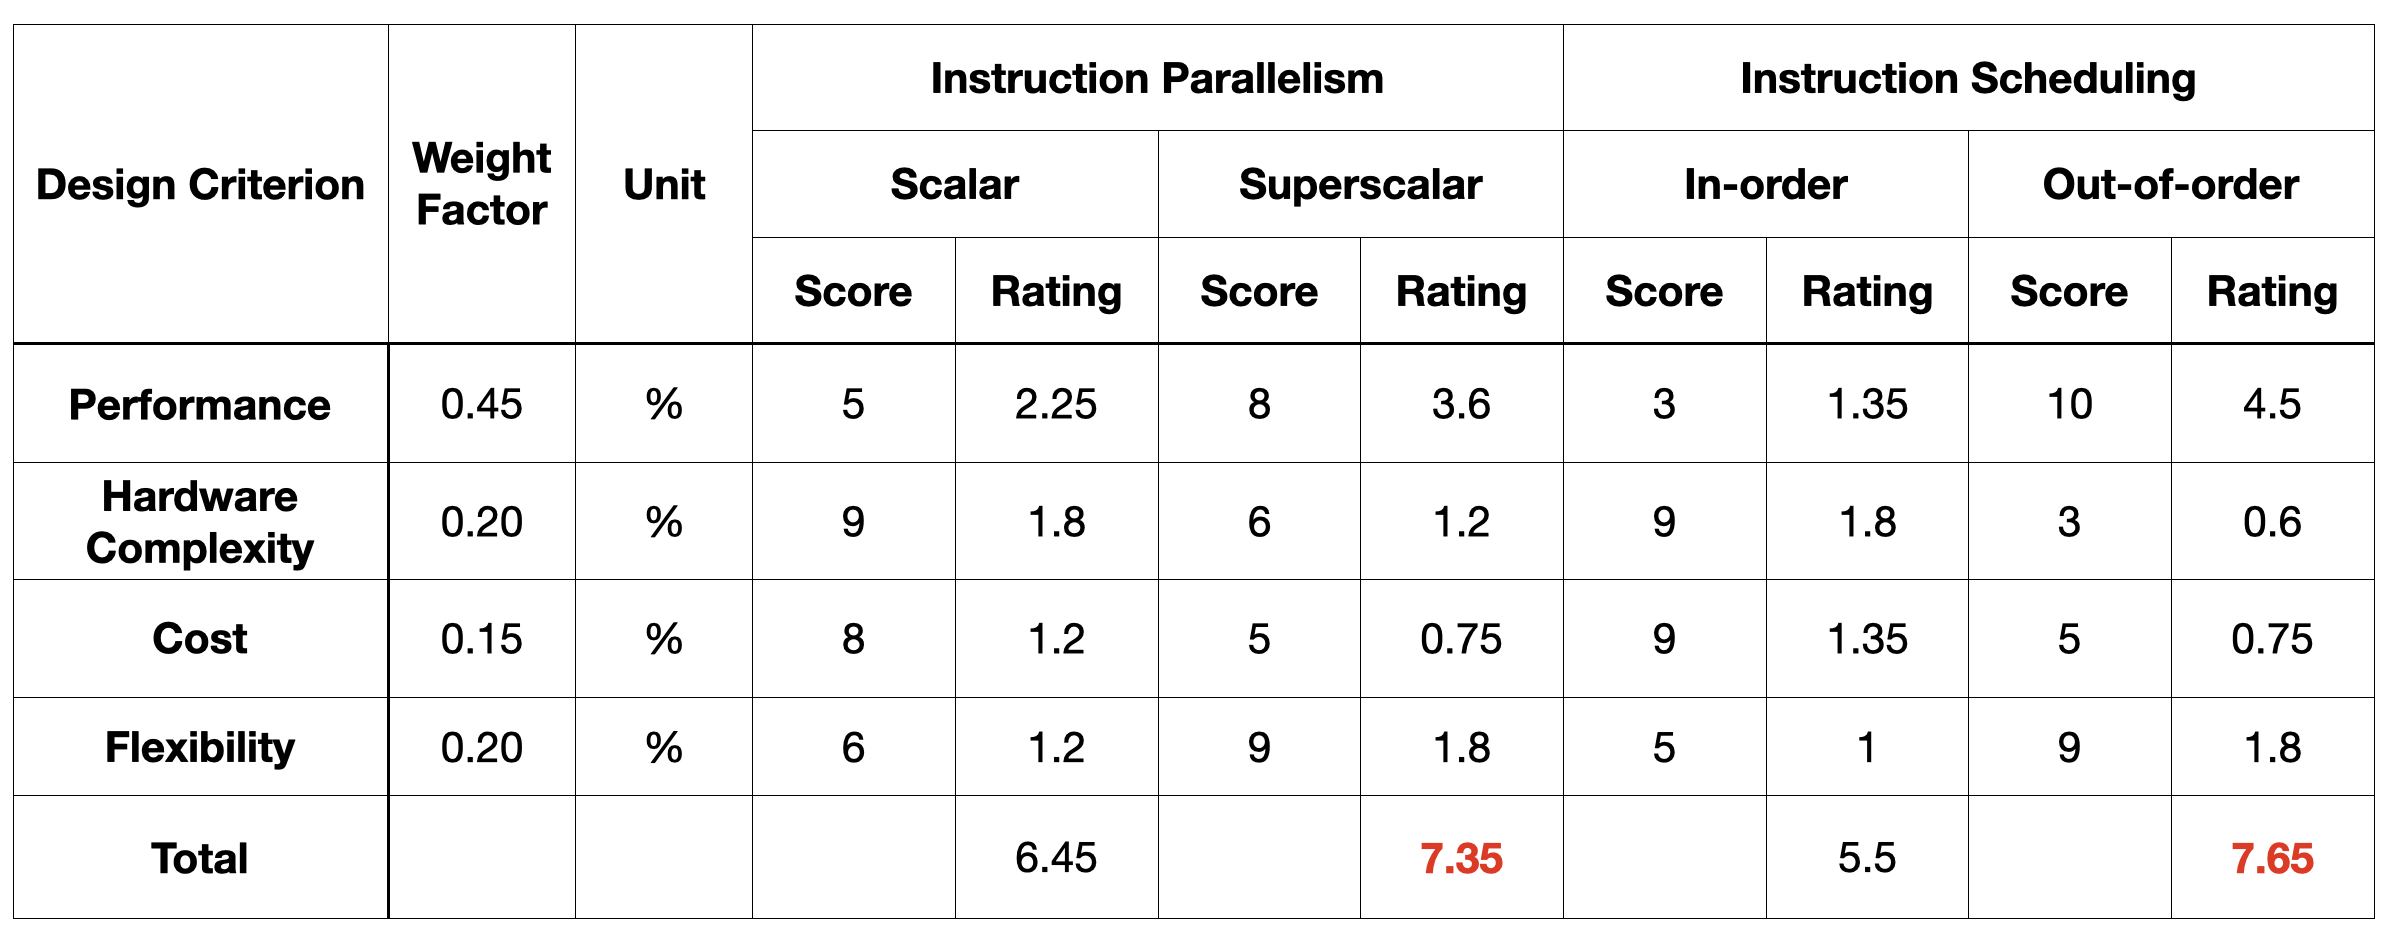
\includegraphics[width=\textwidth]{figure/dm-uarch.png}
    \caption{Decision matrix of microarchitecture design.}
    \label{fig:dm-uarch}
\end{figure}

In the decision matrix, we systematically evaluate our selection on two concepts, i.e., instruction parallelism and instruction scheduling, based on multiple design criterion, including performance, hardware complexity, cost, and flexibility. Based on customer requirements and engineering specifications, we give each criterion a weight factor. As our processor is mainly used for accelerate computing-intensive tasks, performance is the most important evaluation standard, followed by hardware complexity, flexibility and cost. Then, we assess each concept based on a 10-point scale, multiplying by the weight factor and get the rating for each criterion. Finally, we sum the ratings and get the total score of a certain concept design.

For example, in terms of instruction scheduling, in-order design results in good hardware complexity and low cost, but the stalls at different kinds of instruction dependency severely restrict the performance or an in-order processor. On the contrary, the out-of-order design may be complicated to implement in hardware, but results in great performance improvement.

Finally, according to the decision matrix, we choose to implement superscalar and out-of-order features in our processor design.


\section{Verification \& SoC Integration} %yyc

\subsection{Verification}
\subsubsection{Logic Simulation}
Logic simulation is the process to verify the correctness of our processor design. We need a logic simulator that is free to use, so we have following options:
\begin{enumerate}
    \item \textbf{Vivado Webpack Xsim}. Vivado Webpack Xsim is the simulator used in Vivado integrated development environment (IDE). It supports most SystemVerilog features for design and verification. It provides user good experience if they use Vivado IDE to develop and debug, but it also means that users have less flexibility.
    \item \textbf{Icarus Verilog}. It is an open-source Verilog / SystemVerilog logic simulation tool, which converts the Verilog / SystemVerilog source code to an intermediate form and then performs behavioral simulation. It supports both SystemVerilog design language and verification language, but the performance for simulation is relatively low.
    \item \textbf{Verilator}. It is another open-source Verilog / SystemVerilog simulator, which converts Verilog / SystemVerilog models into C/C++ models, and uses C++ as the verification language. Although it does not support the verification language of SystemVerilog, the performance for simulation is satisfying.
\end{enumerate}
There are other commercial software tools for this task. However, all of them require expensive commercial license.

Our final decision is to use both Vivado Webpack Xsim and Verilator. We use Vivado Webpack as it is convenient to debug considerably small design in the Vivado IDE. We choose Verilator to simulate the integrated SoC and use it to build our simulation environment. C++ is a much more powerful language than SystemVerilog, and it brings productivity when we build the simulation system. We do not choose Icarus Verilog due to both its poor performance and its difficulty to integrate with the other parts in the simulation system.

\subsubsection{Functional Verification}
The key part for the functional verification is to choose a proper simulator / emulator as a comparison model. Followings are some popular choices:
\begin{enumerate}
    \item \textbf{Gem5}. Gem5 is an open-source computer architecture simulator used in both academia and industry. It is a very complete but complicate simulator, which provides support for multiple ISAs, including ARM, MIPS, X86, etc. It also provides multiple models for microarchitecture and memory system simulation.
    \item \textbf{Qemu}. Qemu is a popular emulator, which dynamically translate the target binary to the host machine code. Therefore, the user can execute RISC-V programs on a X86 or ARM machine. This emulator can perform not only user level simulation, but also system level simulation.
    \item \textbf{Spike}. Spike is a lightweight simulator, which implements the RISC-V ISA specifications. It is often considered as a golden model for RISC-V ISA.
\end{enumerate}

In this project, we focus on the RISC-V ISA. Also, we use the simulator only to verify the functionality correctness of our design, so we do not need a complicated simulator like gem5. Qemu is an emulator so it cannot provide adequate information about program execution trace, which is a critical part to compare to verify our design. Therefore, our final decision is to use Spike simulator. Spike is also easier to modify and integrate into our simulation system.


\subsection{SoC Integration}
There exists a vast design space for SoC integration, mainly depending on the customer requirements. Our SoC integration and simulation system should be able to complete the following tasks conveniently and efficiently:
\begin{enumerate}
    \item The process of loading and executing program.
    \item The process of reading inputs and saving outputs.
    \item The process of printing messages.
\end{enumerate}
The SoC integration scheme and the whole simulation system integration scheme is thus referred to Spike. Although Spike is an architectural level simulator, its internal structure includes an SoC as well as a well-designed, lightweight simulation environment.

Illustration~\ref{fig:450-soc-sys} is a high-level overview of the simulation environment configuration. This illustration can serve as a description of the system for both our Verilator-based simulation system as well as the Spike simulation model, although the internal details are totally different. The SoC integrates the CPU core with the peripheral devices like RAM and ROM through a system level bus. The simulation environment lies on a host machine, which communicates with the SoC through a pure-software frontend server. The frontend server can perform tasks like loading program into the memory as well as transmitting some requests from the CPU core to the host machine. The program running on the CPU can communicate with the frontend server at system level through global variables in the program. The frontend server will link to those global variables when it loads the program into the RAM. By writing values to and reading values from the global variables, the program can perform tasks like opening a file, writing to a file, etc.

\begin{figure}[!htp]
    \centering
    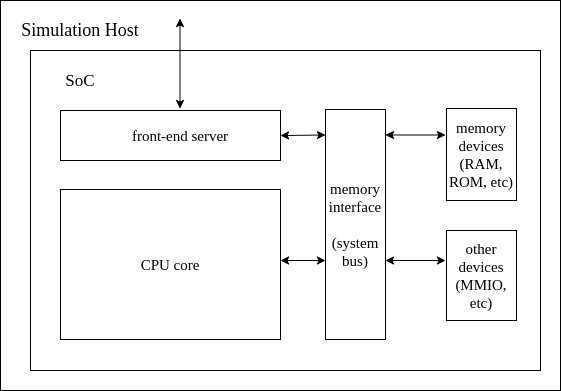
\includegraphics[width=0.8\textwidth]{figure/450-dr3-sys.png}
    \caption{SoC and simulation system integration.}
    \label{fig:450-soc-sys}
\end{figure}

% = = = = = = = = = = = = = = = = = = = = = %
%             Design Description            %
% = = = = = = = = = = = = = = = = = = = = = %

\let\clearpage\relax
\chapter{Final Design Description \& Analysis}

In this chapter, we will review our selected concepts in details, including engineering design analysis, design description and analysis of microarchitecture for each pipeline stages.

\section{Engineering Design Analysis}

\subsection{ISA} %sj
As we mentioned above, we will select our instruction set architecture (ISA) among three choices: MIPS, ARMv7 and RISC-V. Their advantages and disadvantages are listed in Section \ref{section:isa}.

After discussion, we decide to choose RISC-V ISA as our design standard.

Since our final product uses approximate computing unit to accelerate machine learning and neural network, custom ISA is necessary for us. RISC-V supports custom design instructions and also has enough design space compared to other two choices.

Besides, we need to balance our workload and supported features. RISC-V supports many pre-defined instructions, with acceptable complexity. After evaluation, we think we can finish our design and implement on RISC-V in three months.

\subsection{Microarchitecture} \label{section:Microarchitecture}% sl 
We have used the decision matrix to determine the final design of our processor microarchitecture design. Specifically, we determine to implement superscalar and out-of-order features in our design, which matches most of customer requirements. For example, in the aspect of performance, our superscalar out-of-order design provides good performance especially in those computing-intensive tasks. It matches the engineering specifications we set earlier, including supporting instruction dynamic scheduling, etc., and provides a good performance-power-cost balance.

\section{Design Description of Microarchitecture}
In this part, we will explain our design details of each microarchitecture pipeline stages. A simplified pipeline design diagram is shown in Fig.~\ref{fig:pipeline}. Our processor supports 4-way superscalar execution and instruction dynamic scheduling, dividing into two parts: frontend and backend. In the frontend, there are 4 stages: instruction fetch (IF), instruction decode (ID), register renaming (RR), dispatch (DP). In the backend, there are 5 stages: issue (IS), register file (RF), execution (EX), write back (WB), and commit (CM).

\begin{figure}
    \centering
    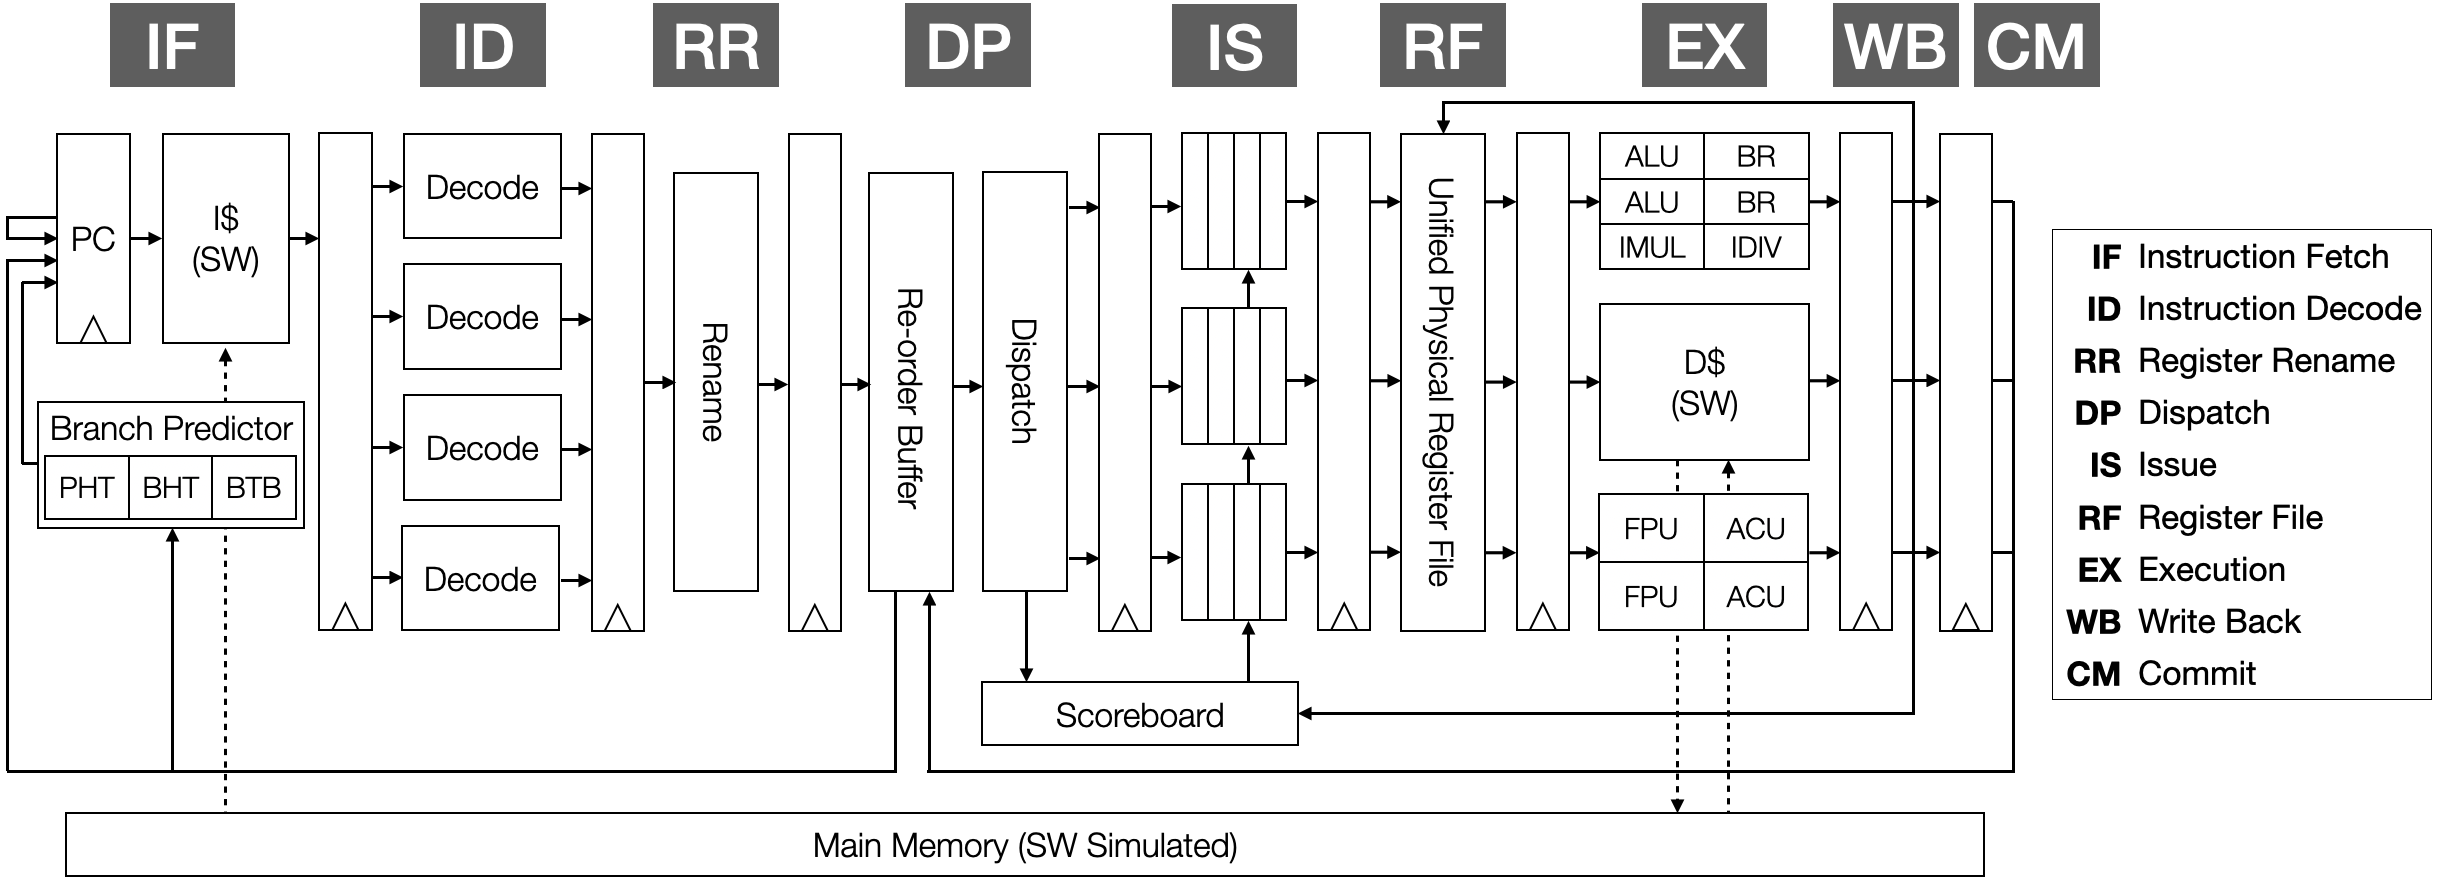
\includegraphics[width=\textwidth]{figure/design.png}
    \caption{Simplified pipeline diagram.}
    \label{fig:pipeline}
\end{figure}

\subsection{Instruction Fetch \& Branch Prediction} % syq
The Instruction Fetch stage is the first stage of the whole pipeline (Fig. \ref{fig:pipeline}). It reads instructions from memory. The branch predictor is also included into this stage. As is shown in Fig. \ref{fig:br_pred}, the branch predictor consists of Direction Predictor and Branch Target Table (BTB). The Direction Predictor uses 2 bits to represent the possibility of branch taken: 00 - strongly not taken, 01 - weakly not taken, 10- weakly taken, 11- strongly taken. We decides what is the next PC to read based on the mis-predict feedback from Reorder Buffer and the predict output of the branch predictor.
\begin{figure}[!htp]
    \centering
    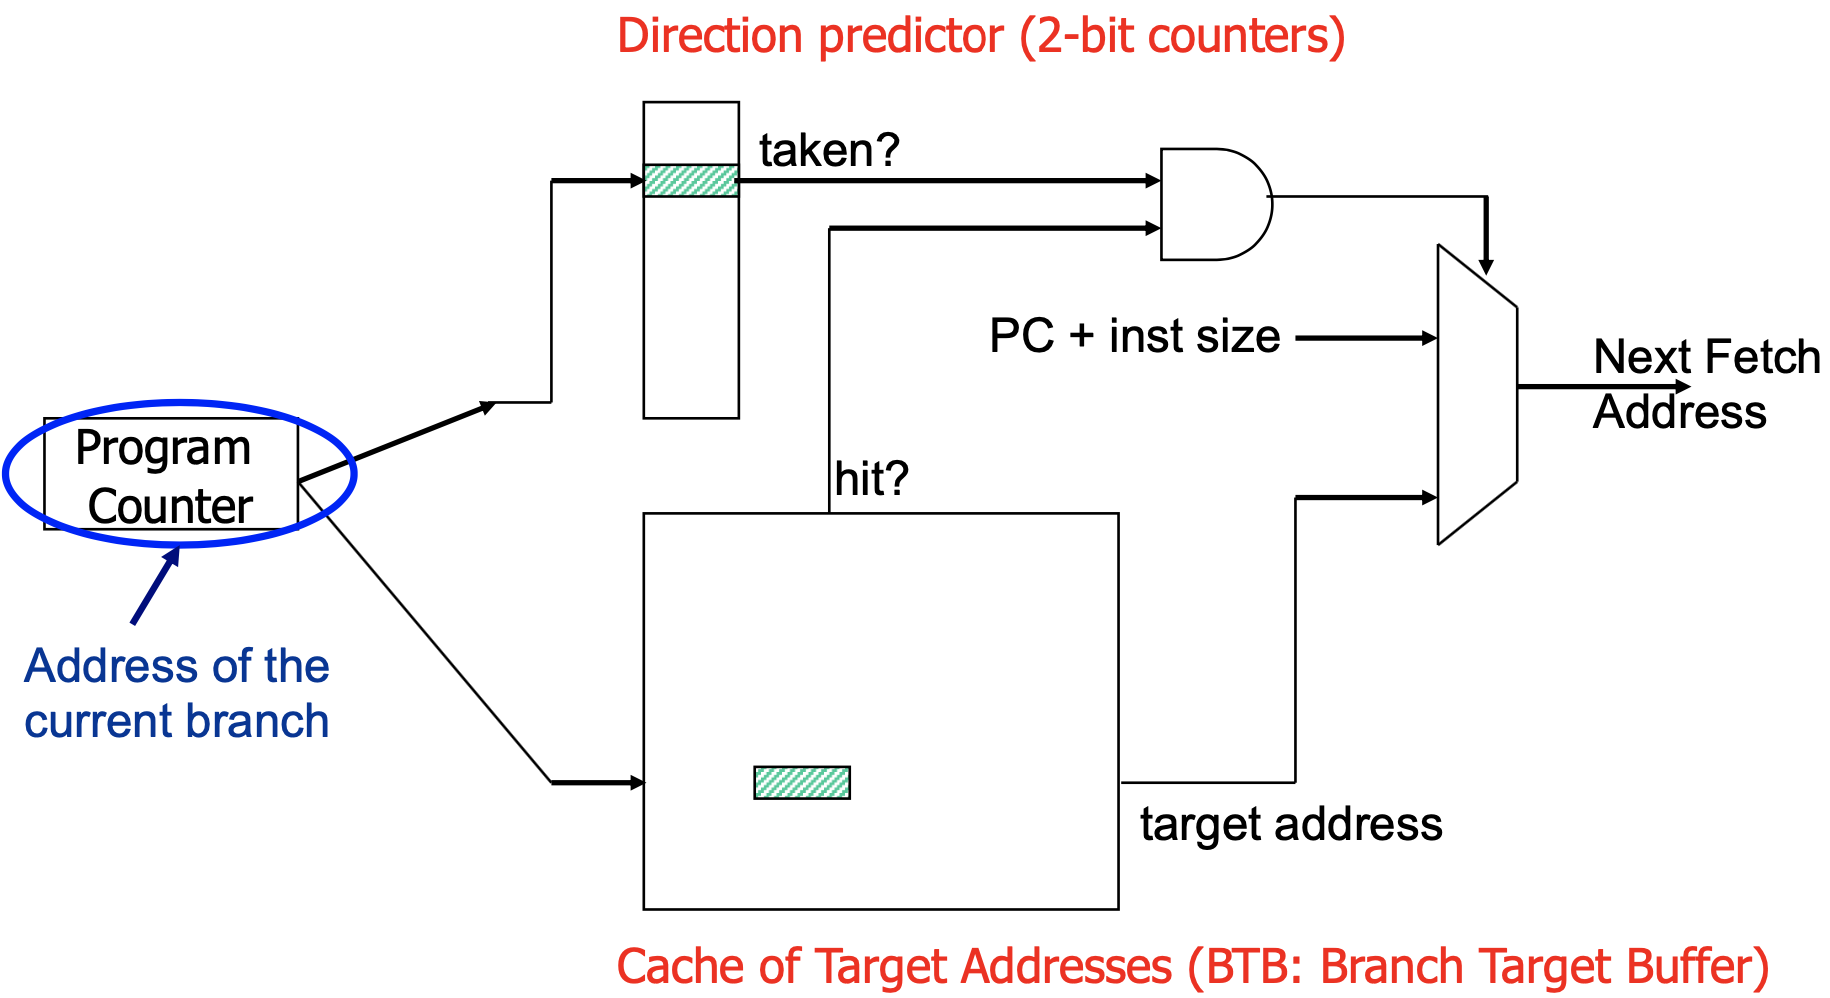
\includegraphics[width=0.8\textwidth]{figure/branch_predictor.png}
    \caption{Branch predictor diagram.}
    \label{fig:br_pred}
\end{figure}

\subsection{Fetch Buffer} % syq
The Fetch Buffer serves as a buffer to store the fetched instructions if they can not be dispatched at once due to the congestion of later stages. The buffer is implemented as a First-In-First-Out (FIFO) queue to ensure an in-order dispatch of instructions.

\subsection{Instruction Decode} %sj
In this part, we decode the input instructions into micro operations (\texttt{uops}). We use four decoders to make sure that four instructions can be decoded at the same time.

\begin{figure}[!htp]
    \centering
    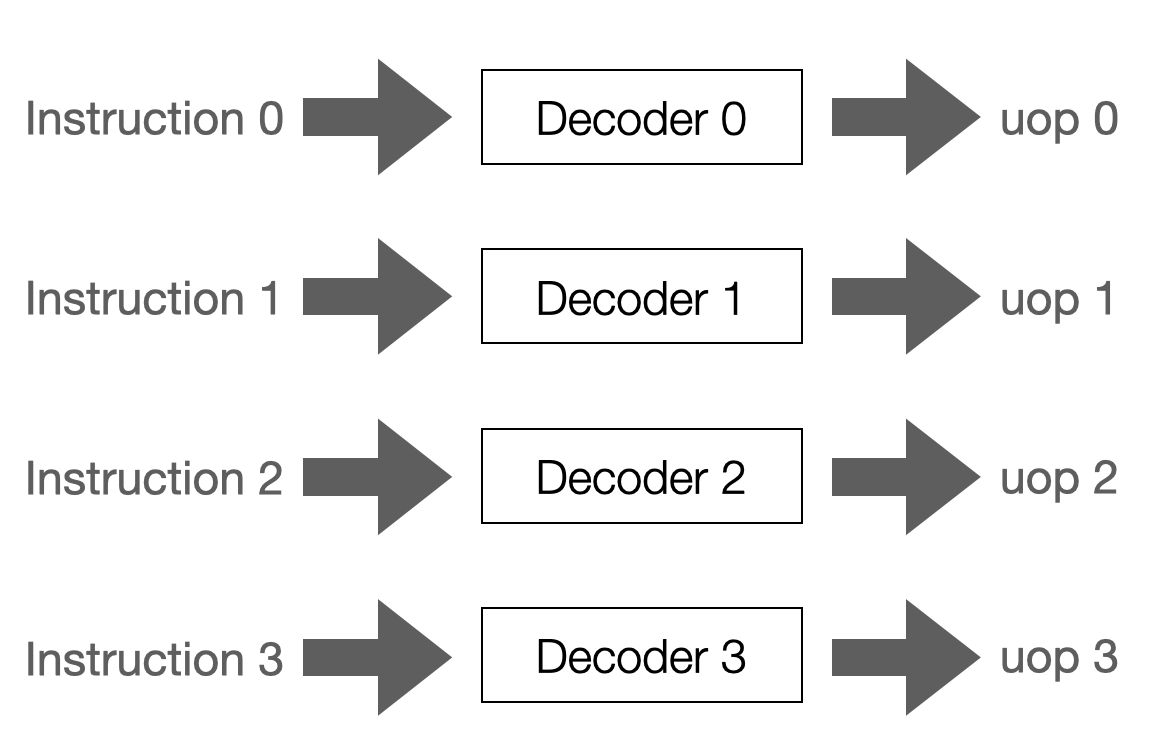
\includegraphics[width=0.5\textwidth]{figure/decode.png}
    \caption{4-way decoder.}
    \label{fig:decoder}
\end{figure}

RISC-V instructions can be classified by their formats. Fig.~\ref{fig:RISCV_inst} shows all instruction types. The decoders will first sort input instructions according to the format table. Then, the decoders will analyze information in each part of the instruction and translate them into micro operations that can be understood by the following stages.

\begin{figure}[!htp]
    \centering
    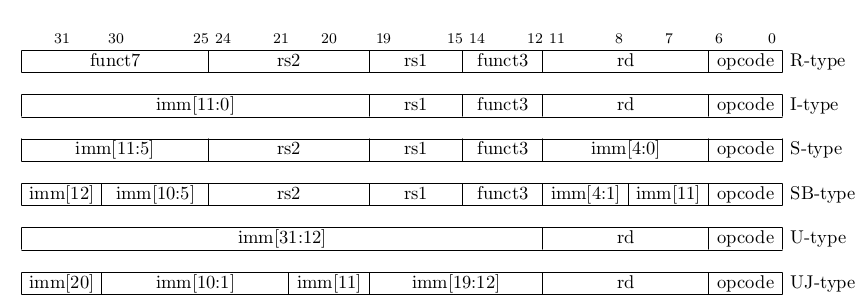
\includegraphics[width=0.85\textwidth]{figure/riscv-isa.png}
    \caption{RISC-V instruction format\cite{RISC-V_unprivileged_ISA}.}
    \label{fig:RISCV_inst1}
\end{figure}

Micro operations are designed as a data structure, including source architectural registers, destination register, used immediate and operation code. Therefore, other stages can fetch needed information quickly and accurately from micro operations.

\subsection{Register Rename} % sj
In this part, we rename architectural registers and assign them with physical registers. Besides, the rename part should also free physical registers that are retired by committed instructions.

The main purpose of register rename is to break the anti-dependency (write after read, WAR) and output dependency (write after write, WAW) between architectural registers. Therefore, instructions with these dependencies can be pipe-lined together in execution stage, which will improve the performance of the processor. Fig.~\ref{fig:waw_war} shows how to break WAR and WAW in the rename stage. On the other hand, the rename part should protect and record the true dependency (read after write, RAW) so that an instruction can read and get the right source register. For special architectural register, i.e., \texttt{x0}, the rename part should protect it to be assigned to other physical registers.

\begin{figure}[!htp]
    \centering
    
\includegraphics[width=0.5\textwidth]{figure/waw.png}
    
\includegraphics[width=0.5\textwidth]{figure/war.png}
    \caption{Write after read and write after write dependency.}
    \label{fig:waw_war}
\end{figure}

Our rename part is an ``explicit renaming'' or ``physical register file'' out-of-order core design. A physical register file (128 entries), containing many more registers than the ISA dictates (32 entries for integer and 32 entries for floating points), holds both the committed architectural register state and speculative register state. The retirement rename allocation table (rRAT) contains the information needed to recover the committed state. The mapping relation will be recorded in the mapping table, also called rename allocation table (RAT). As instructions are renamed, their register specifiers are explicitly updated to point to physical registers located in the physical register file. Fig.~\ref{fig:rename} shows the rename logic between two instructions and their architectural registers. Since our rename stage has four ways and can rename four instructions at the same time, the final logic is far more complex than the given example.

Since we use unified physical register file in issue stage, integer architectural registers and floating point architectural registers share the same register ``pool'' and address structure. For this reason, we also rename their physical registers together and do not take their differences into consideration in rename stage.

\begin{figure}[!htp]
    \centering
    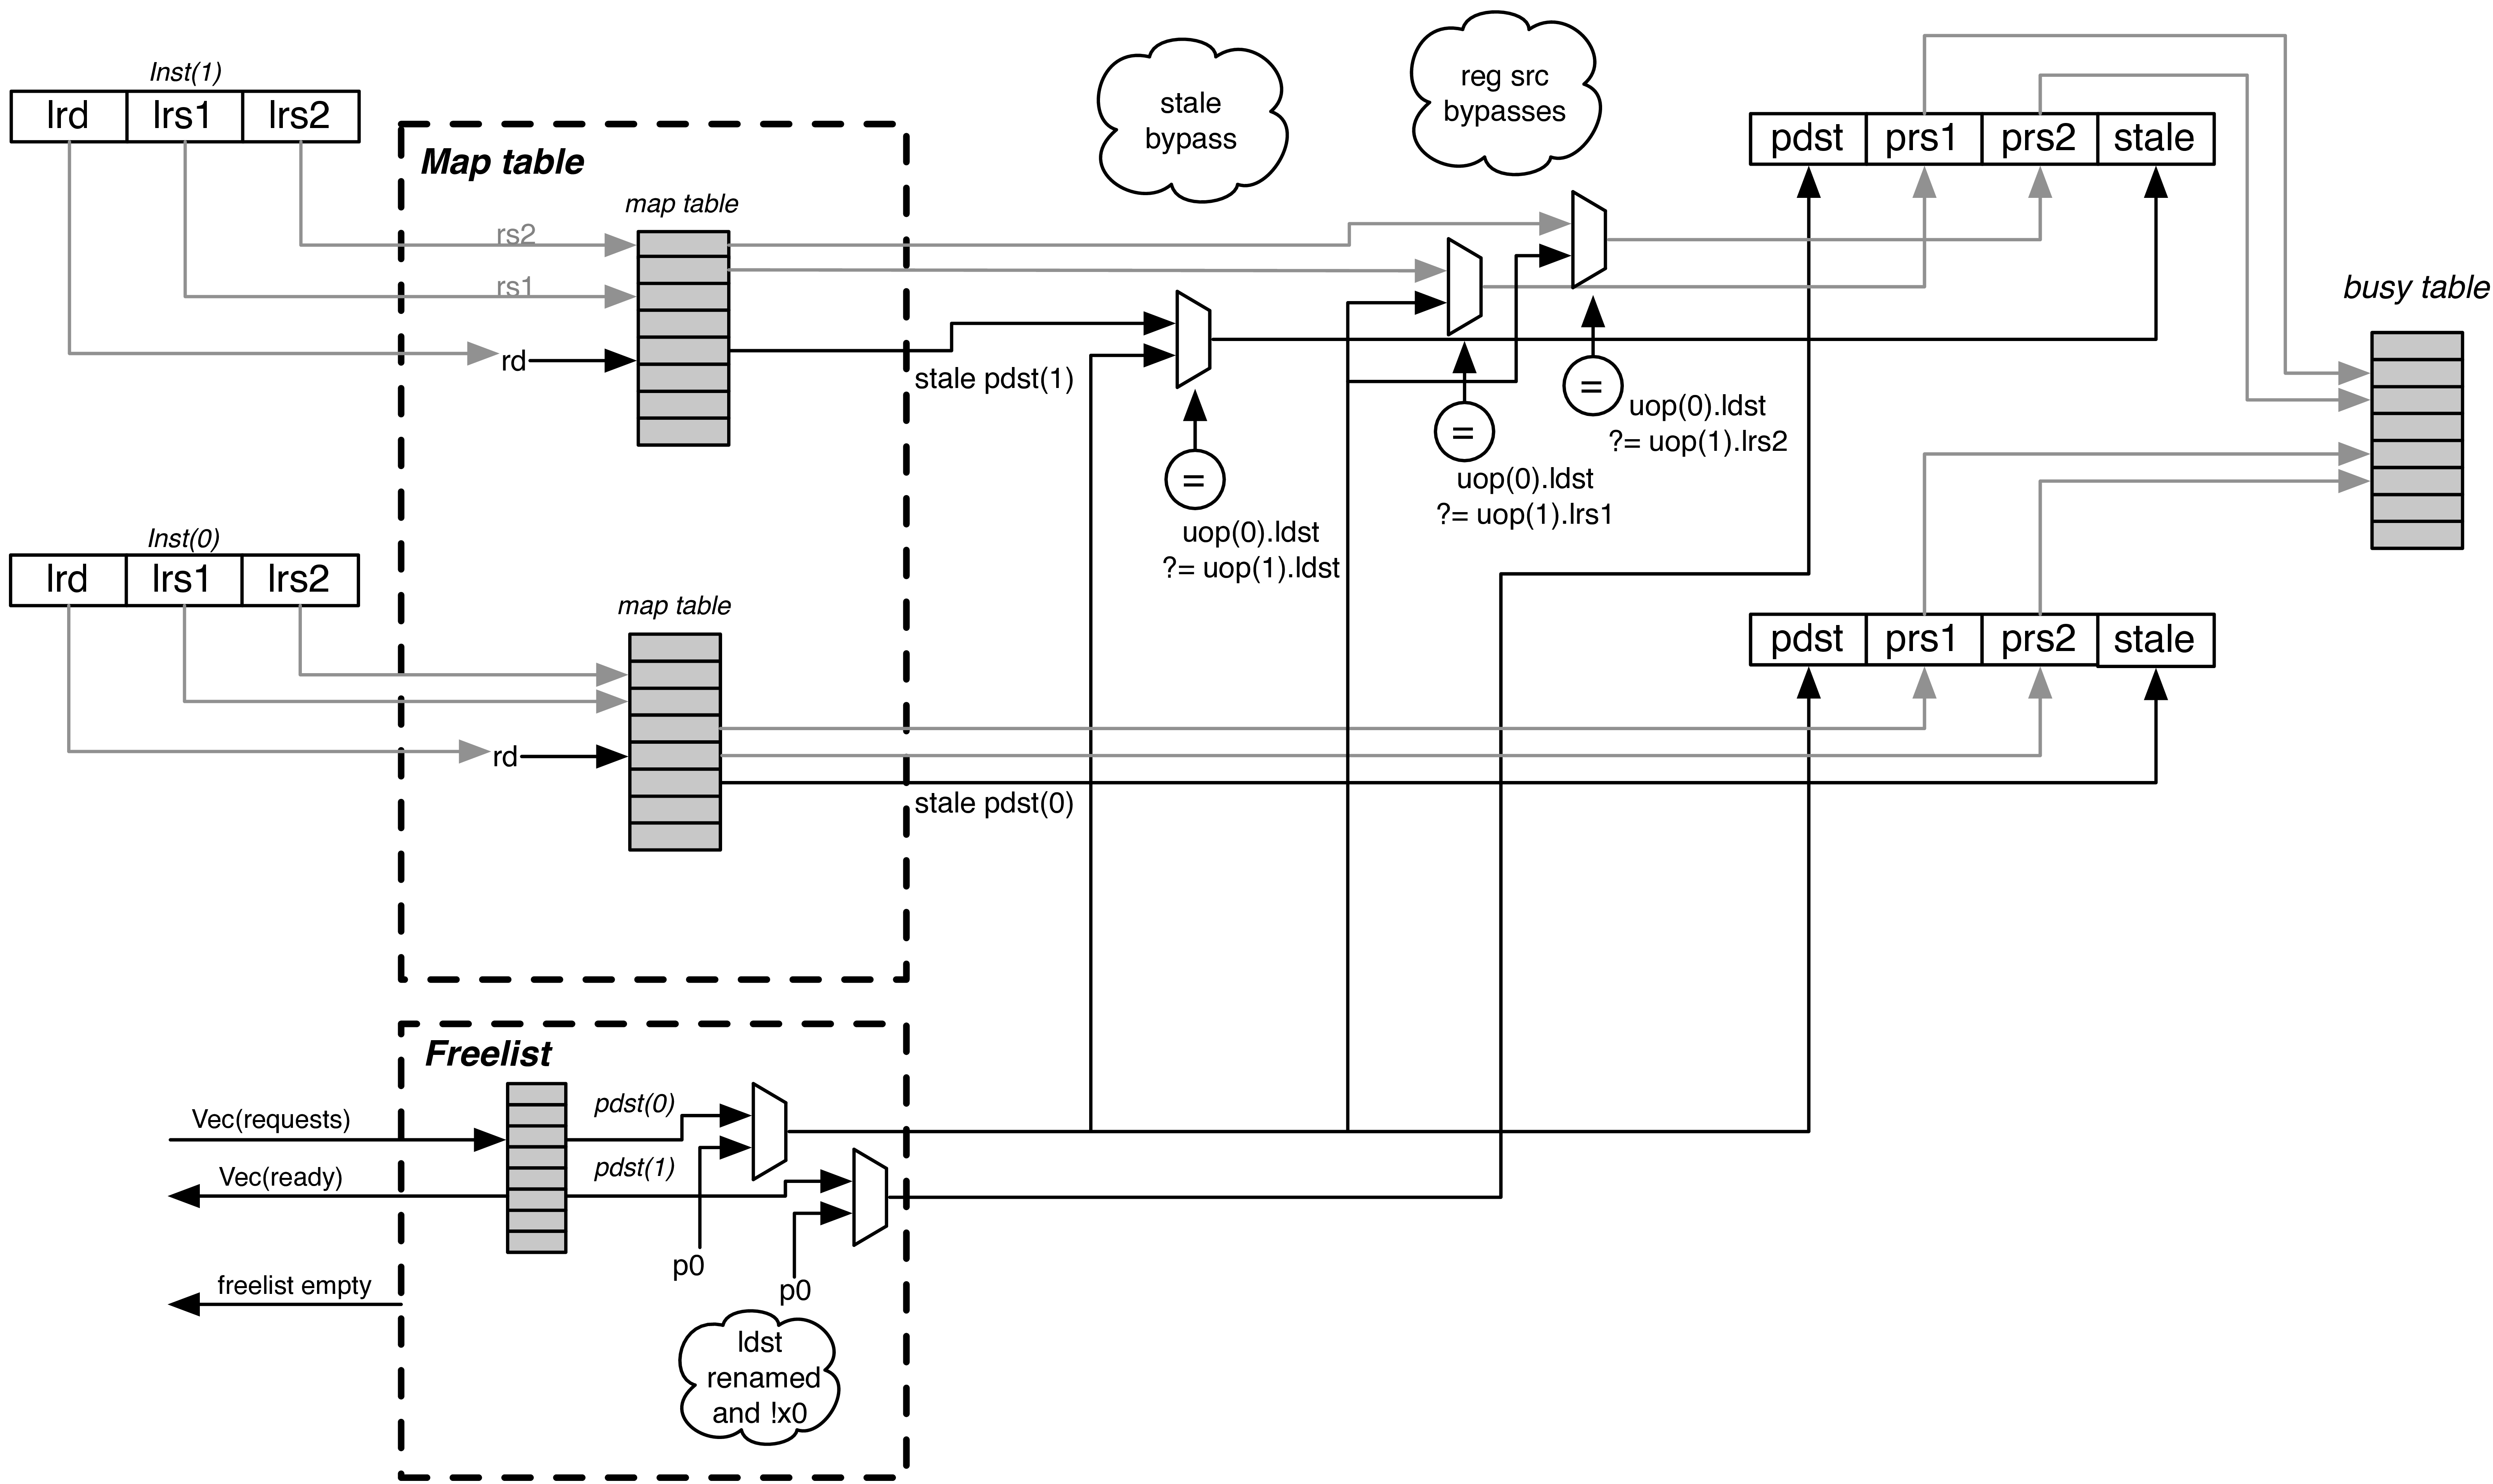
\includegraphics[width=0.8\textwidth]{figure/rename-pipeline.png}
    \caption{Register rename logic\cite{Boom}.}
    \label{fig:rename}
\end{figure}

We use a free list to record the usage of physical registers. When a physical register is assigned to an architecture register, it will be marked as ``busy'' in the free list. On the other hand, when it is retired by the retired instructions, it will be marked as ``free''. Fig.~\ref{fig:mapping} shows the relation between mapping table, free list and rRAT.

\begin{figure}[!htp]
    \centering
    
\includegraphics[width=0.65\textwidth]{figure/map_rename.png}
    \caption{Rename stage with free list, mapping table and rRAT.}
    \label{fig:mapping}
\end{figure}

To avoid data hazards and risks, we use a conservative strategy. When an architectural register $x_a$ is re-assigned to a new physical register $r_b$, its previous physical register $r_a$ will be recorded. Cycles later, when the architectural register $x_a$ is retired by its instruction, its previous physical register $r_a$ will be freed or assigned to another architecture register. At that time, the free list or the mapping table is updated by the new mapping relation. Besides, rRAT is also refreshed by the mapping relation between architectural register $x_a$ and its new physical register $r_b$ so that the rename stage can quickly recover from mis-prediction, interrupts or exceptions.

When a mis-prediction happens, the mapping table and the free list will recover their mapping relation and free stages from rRAT. The recover process takes only one clock cycle, which means that our rename stage can quickly response to mis-prediction, interrupts or exceptions. This feature can reduce our instructions per cycle (IPC) in programs with many branch mis-predictions or interrupts.

\subsection{Dispatch} %sl

Dispatch is the last stage in the frontend and also the last in-order stage. In this part, we write the instructions from the previous stage into the re-order buffer (ROB) the backend and then dispatch these instructions to the corresponding issue units according to the \texttt{iq\_code} field in the uops. We support dispatching 4 instruction at one time. To reduce the logic complexity of input selection in the issue stage, we design our dispatch stage based on collapsing logic, shown in Fig.~\ref{fig:dp-1}. The instructions will always be dispatched to the top space in the inputs of backend without any bubbles.

\begin{figure}[!htp]
    \centering
    \begin{subfigure}{0.45\textwidth}
        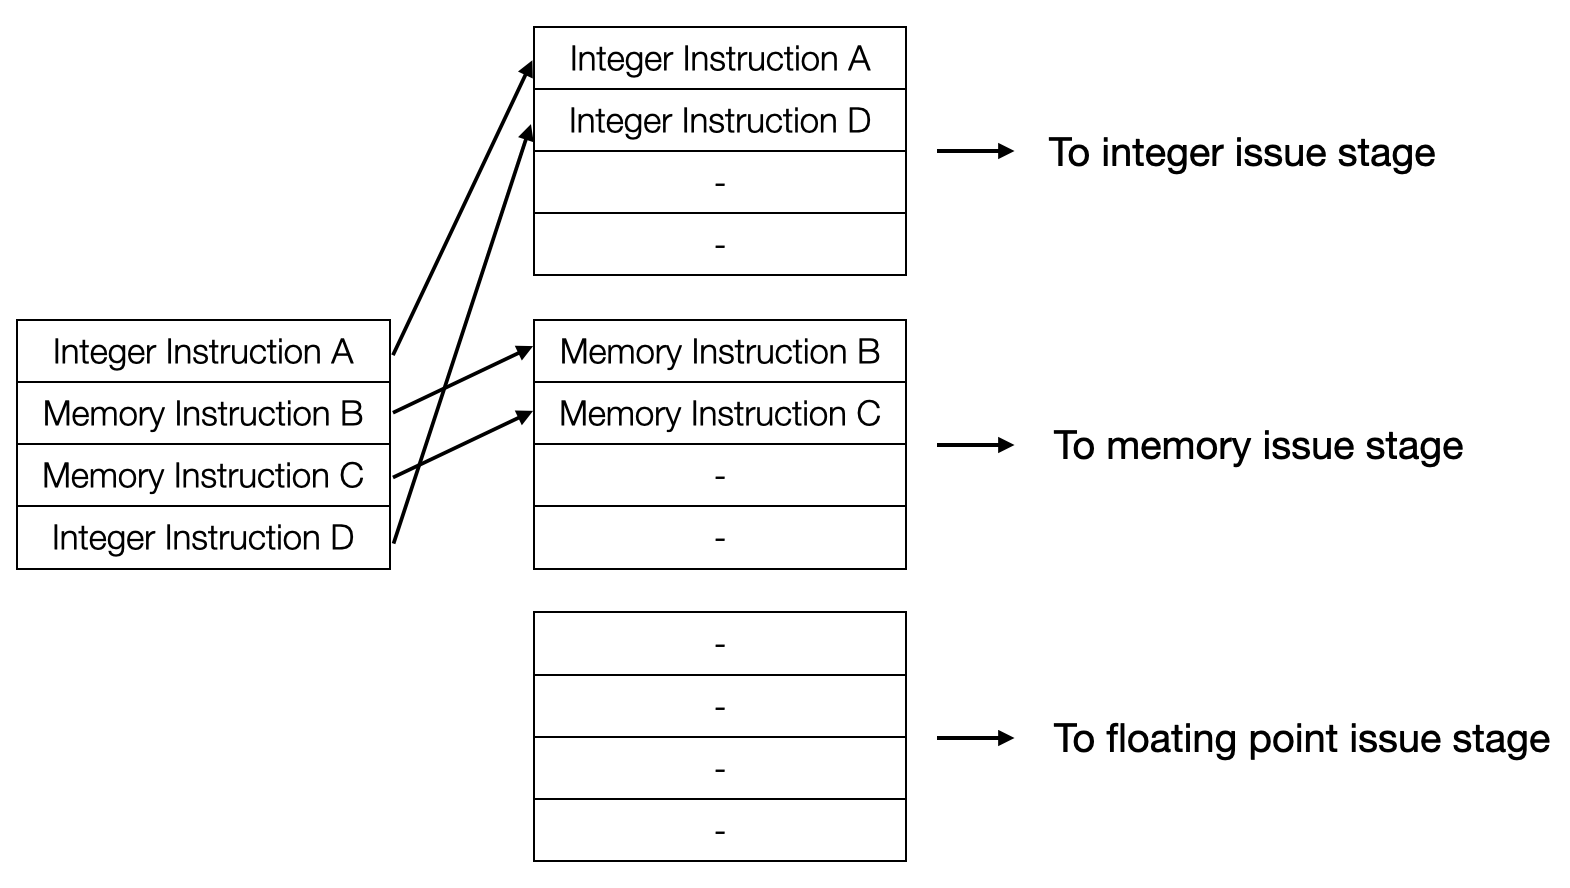
\includegraphics[width=\textwidth]{figure/dispatch.png}
        \caption{Collapsing dispatch logic.}
        \label{fig:dp-1}
    \end{subfigure}
    ~
    \begin{subfigure}{0.45\textwidth}
        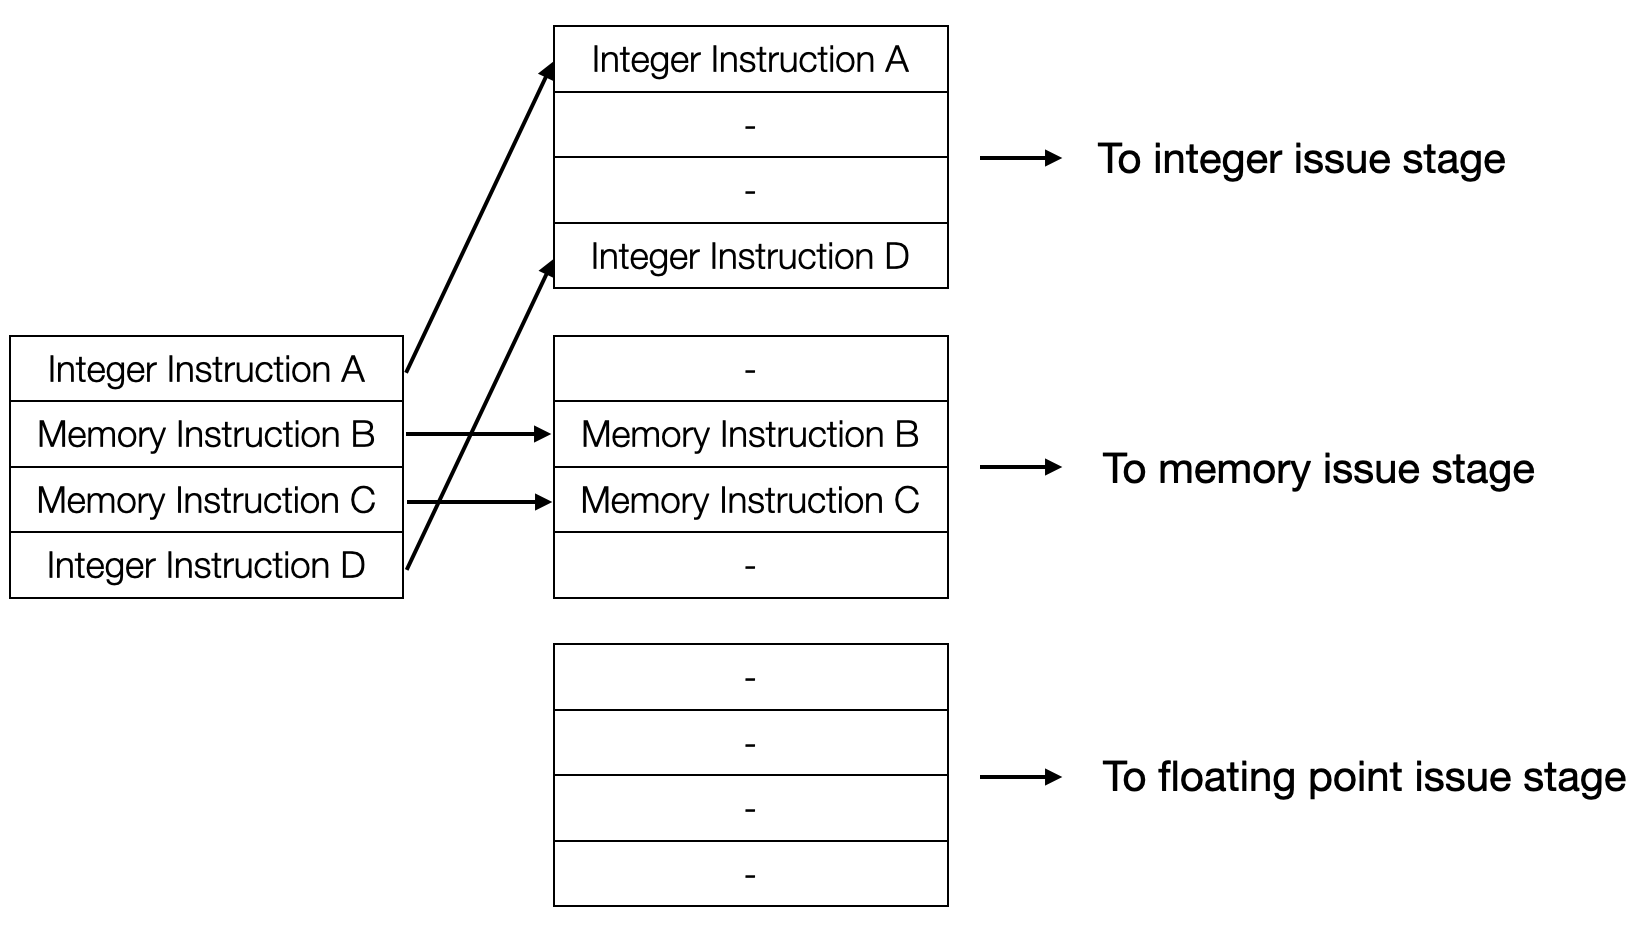
\includegraphics[width=\textwidth]{figure/dispatch-nc.png}
        \caption{Non-collapsing dispatch logic.}
        \label{fig:dp-2}
    \end{subfigure}
    \caption{Two different dispatch logic design.}
    \label{fig:dispatch}
\end{figure}

On the contrary, a non-collapsing dispatcher is shown in Fig.~\ref{fig:dp-2}. The logic is simpler, but it will further complicate the input selection logic and increase the delay in issue stage, especially for memory instructions, which usually require strict memory access order to keep the consistency.


\subsection{Issue} %sl
In this part, we accept the instructions from the frontend, track the data and structure dependency between instructions, select part of the ready instructions and issue them to the register file and the execution units. This is also the critical point between in-order and out-of-order stages in our microarchitecture design, and is the key component to implement out-of-order scheduling algorithm.

In our design, we implement 3 issue units: integer issue unit, memory issue unit and floating point issue unit. All 3 issue units are able to accept four instructions at one time, but the outputs differ, dependent on the design of execution units.

\subsubsection{Issue Unit for Integer \& Floating Point} %sl
We design the input selection logic to assign the input instructions to free space in the issue units. The logic of instruction assignment is simple. We just put the instructions in the free space from top to bottom. Meanwhile, we design the output selection logic to issue instructions whose dependency is ready to the subsequent pipeline stages. The output width depends on the execution width. In our design, we can issue at most 3 integer instructions or 2 floating point instructions simultaneously. Among all the ready instructions, we also select from top to bottom. A simple example of issue unit for integer instructions is shown in Fig.~\ref{fig:iq-int}.

\begin{figure}[!htp]
    \centering
    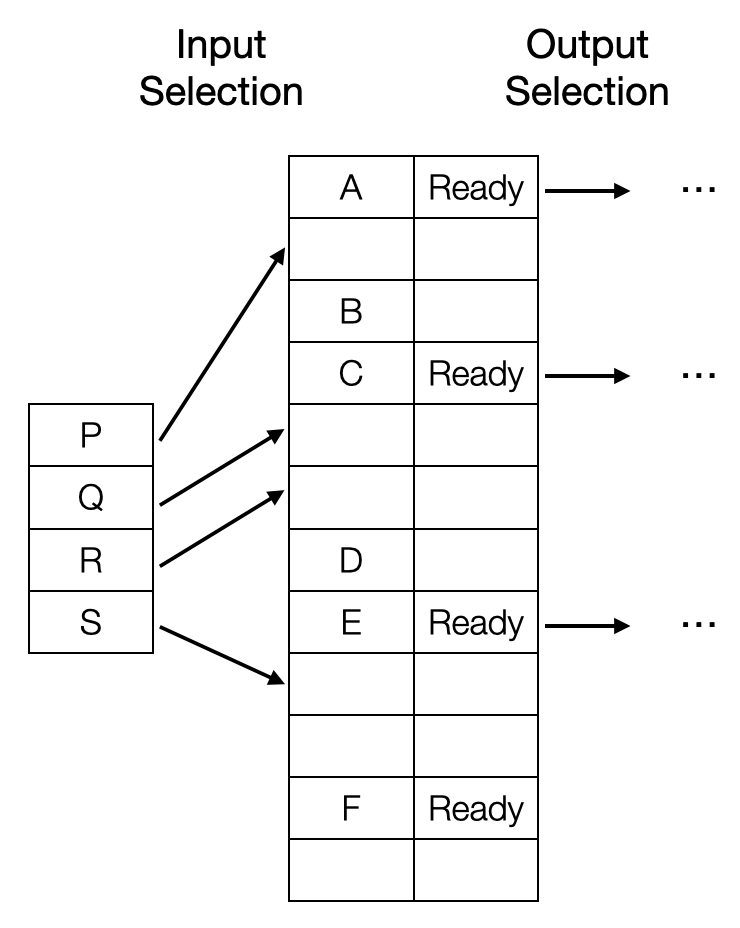
\includegraphics[width=0.3\textwidth]{figure/iq1.png}
    \caption{Example of issue unit logic for integer instructions (L for load and S for store).}
    \label{fig:iq-int}
\end{figure}

\subsubsection{Issue Unit for Memory Access} %sl
Due to the special characteristics of memory access instructions, the selection logic of the issue unit for memory access is different from the logic of the other two issue units. The main principle is to keep the memory consistency, which is a big challenge for out-of-order execution design. It is easy to track data dependency in registers, but it is much more difficult to track the dependency in memory. For example, assuming that the same memory address is stored in the registers \texttt{x1} and \texttt{x2}, for the case that we first store the data to \texttt{[x4]} and then load the data from \texttt{[x3]}, we cannot directly determine whether there exists potential dependency between the two instructions. 

Thus, in our processor design, we use a relatively conservative way to achieve memory consistency. We consider each store instruction as a barrier, i.e., while load instructions can be executed out-of-order, we can issue the store instructions only when it is at the top of our issue unit. As a result, similar to dispatch unit, we design a collapsing structure in the issue unit for memory access. Each time one instruction is issued, all the instructions are ``compressed'' to the top, and the input instructions are added to the tail of the unit. For the output selection logic, if there are remaining store instructions, only the store instruction at the top or the load instructions before any store instructions can be issued.

A simple example is shown in Fig.~\ref{fig:iq-mem}. At the top of the issue unit is a store instruction, which will be issued in this clock cycle. Then all the remaining instructions are pushed to the top, and new instructions are added below.

\begin{figure}[!htp]
    \centering
    \begin{subfigure}{0.4\textwidth}
        \centering
        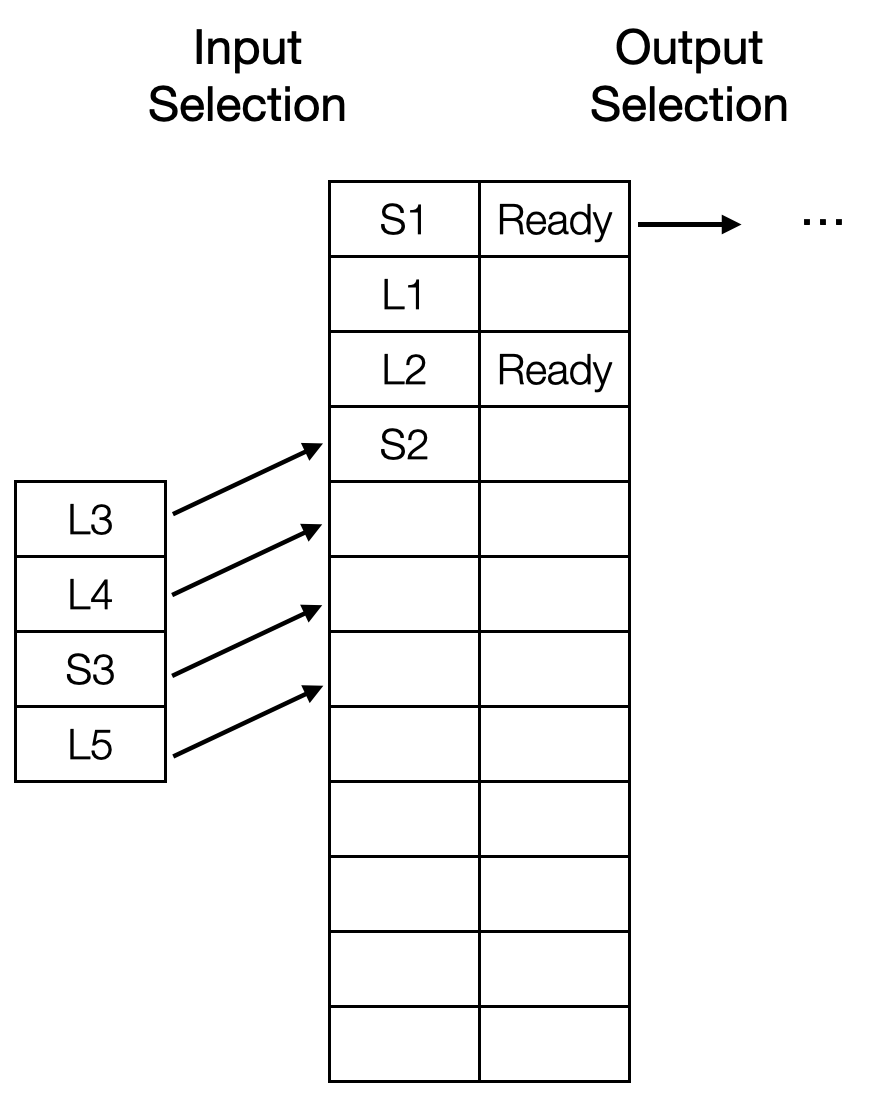
\includegraphics[width=0.75\textwidth]{figure/iq2.png}
        \caption{Example of issue unit logic: stage 1.}
        \label{fig:iq-mem-1}
    \end{subfigure}
    ~
    \begin{subfigure}{0.4\textwidth}
        \centering
        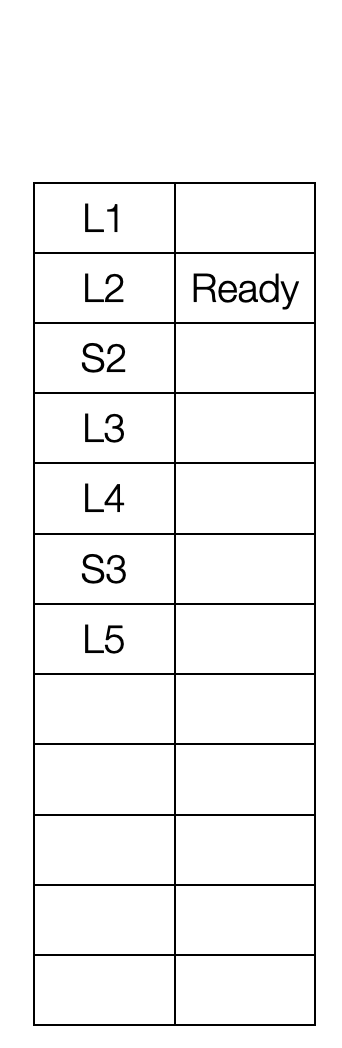
\includegraphics[width=0.3\textwidth]{figure/iq3.png}
        \caption{Example of issue unit logic: stage 2.}
        \label{fig:iq-mem-2}
    \end{subfigure}
    \caption{Example of issue unit logic for memory access.}
    \label{fig:iq-mem}
\end{figure}


\subsubsection{Scoreboard} %sl
Although register renaming may resolve anti-dependency and output dependency, it cannot resolve true dependency, i.e., read-after-write (RAW) dependency, which is usually the crucial bottleneck to further improve instruction level parallelism. In our design, scoreboard is mainly used for tracking data dependency between instructions and sending wake-up signals to the issue units.

The width of scoreboard matches the depth of our physical register file. First, it accepts input from dispatch stage, which is the last in-order stage and sets the busy bits in the scoreboard. Second, it accepts input from write back stage, which clears the busy bits in the scoreboard. Finally, it accepts the query requests from the issue units and returns whether the requiring source registers are ready or not.

Fig.~\ref{fig:sb} shows an example of how scoreboard helps to track RAW dependency between two instructions. Here the second instruction depends on the result of the first instruction. First, when the two instructions enter the dispatch stage, set both \texttt{X} and \texttt{Y} as busy, marking them as in-flight instructions (Fig.~\ref{fig:sb-1}). Second, the first instruction is issued to the later stages of the pipeline (Fig.~\ref{fig:sb-2}). Third, when the first instruction is completed and write back to the register file, set \texttt{X} as not busy (Fig.~\ref{fig:sb-3}). At last, as \texttt{X} is not busy any more, the second instruction checks the scoreboard, finding that it is also ready to issue, and we issue it to the register file and corresponding execution units (Fig.~\ref{fig:sb-4}).

\begin{figure}[!htp]
    \centering
    \begin{subfigure}{0.4\textwidth}
        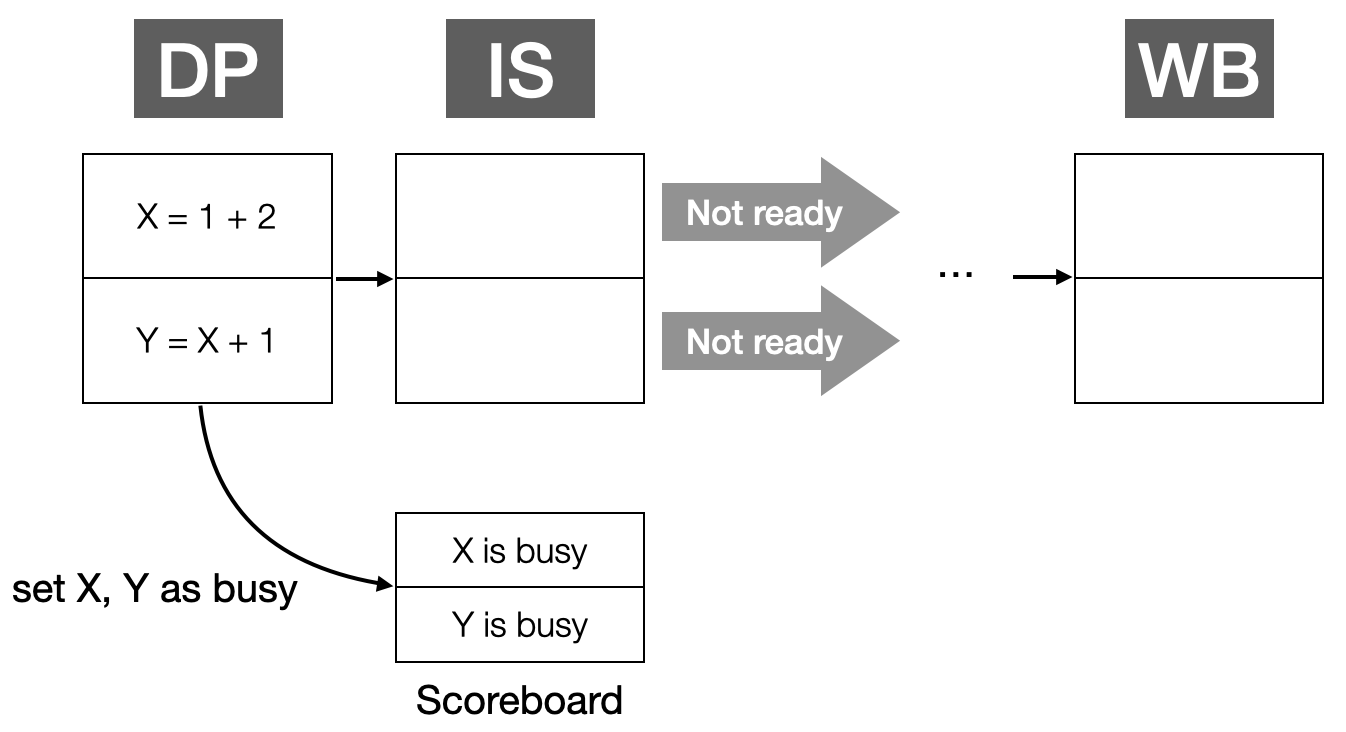
\includegraphics[width=\textwidth]{figure/sb1.png}
        \caption{Example of scoreboard: stage 1.}
        \label{fig:sb-1}
    \end{subfigure}
    ~
    \begin{subfigure}{0.4\textwidth}
        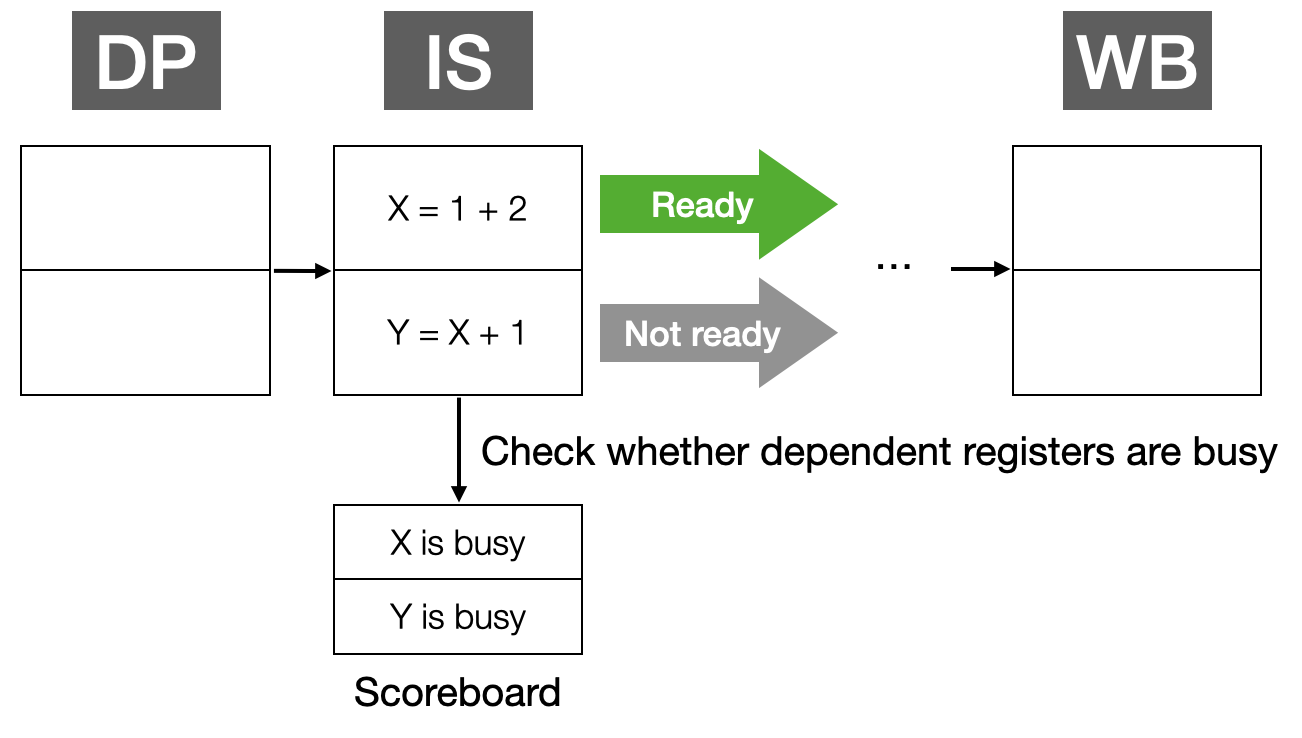
\includegraphics[width=\textwidth]{figure/sb2.png}
        \caption{Example of scoreboard: stage 2.}
        \label{fig:sb-2}
    \end{subfigure}
    
    \begin{subfigure}{0.4\textwidth}
        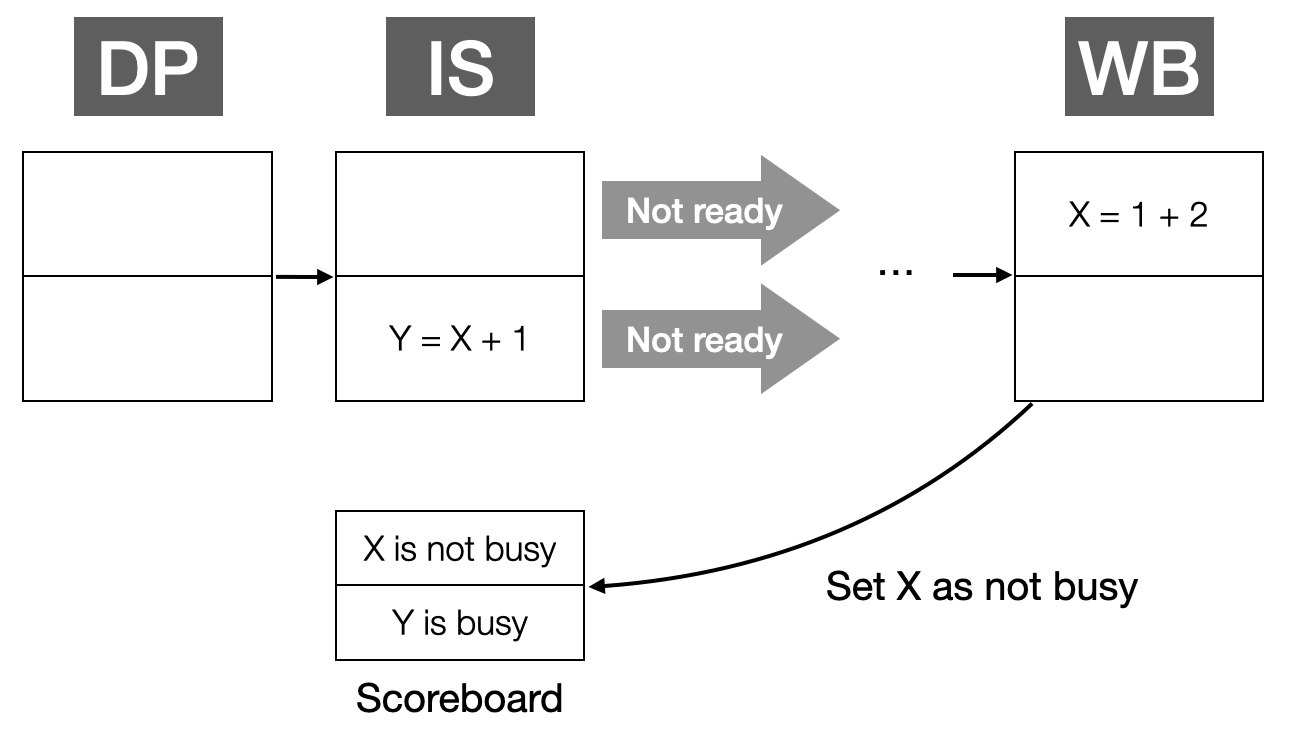
\includegraphics[width=\textwidth]{figure/sb3.png}
        \caption{Example of scoreboard: stage 3.}
        \label{fig:sb-3}
    \end{subfigure}
    ~
    \begin{subfigure}{0.4\textwidth}
        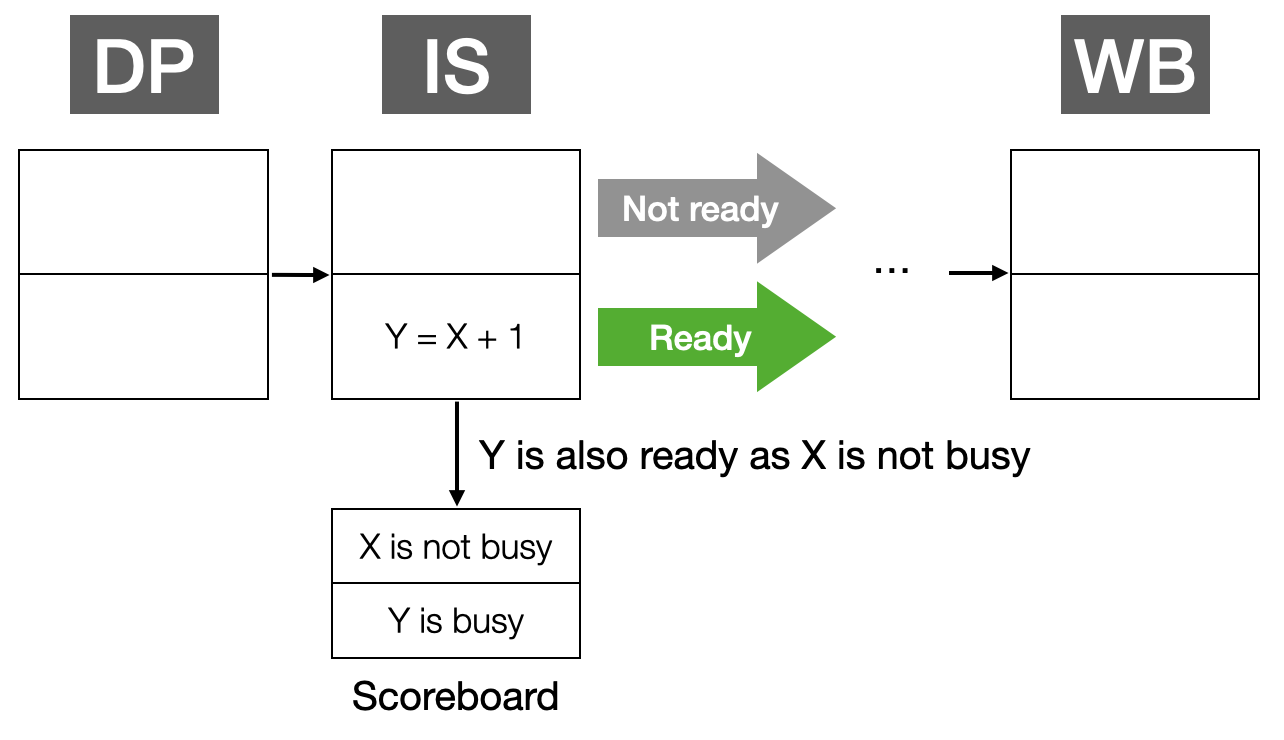
\includegraphics[width=\textwidth]{figure/sb4.png}
        \caption{Example of scoreboard: stage 4.}
        \label{fig:sb-4}
    \end{subfigure}
    \caption{RAW dependency tracking with scoreboard.}
    \label{fig:sb}
\end{figure}

\subsection{Register File} %sl

As mentioned in the register rename part, our processor resolves anti-dependency and output dependency based on physical register file (PRF). In our design, there is only one unified PRF with 128 entries. Bypassing logic is implemented to handle the case that source operands are identical with destination operands. 

Compared to other methods of register renaming, there are several advantages of using PRF. There is no need to move the data frequently, as the data always stays in the PRF. We don't need to add selectors for instructions to determine which register file to use. Furthermore, It is also easy to recover from branch mis-predictions, which helps to further explore the instruction level parallelism and improve the performance.

\subsection{Execution} %sl

An execution pipe is a set of function units. In our microarchitecture design, we have 6 execution pipes in total (3 for integer, 1 for memory access and 2 for floating point), shown in Fig.~\ref{fig:pipe}.

\begin{figure}[!htp]
    \centering
    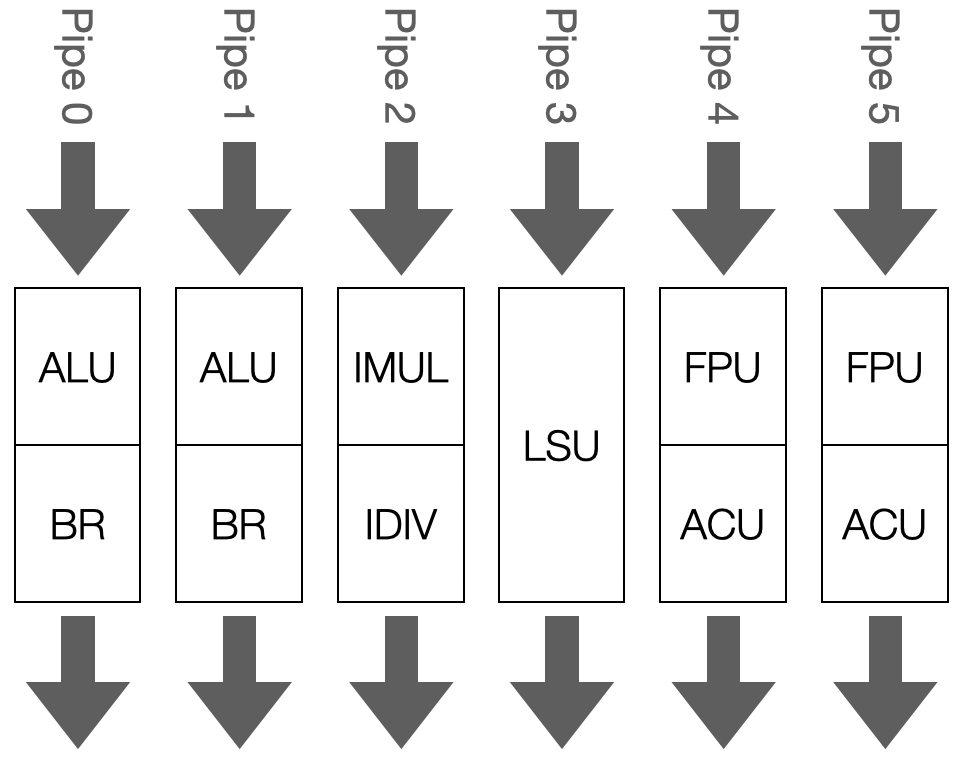
\includegraphics[width=0.4\textwidth]{figure/pipe.png}
    \caption{Execution pipes.}
    \label{fig:pipe}
\end{figure}

\subsubsection{Execution Units for Integer} % sl
There are 3 pipes for integer instructions. Pipe 0 and 1 encapsulate arithmetic logic units (ALU), which perform normal integer arithmetic operations except multiplication and division, and branch units, while pipe 2 is used for integer multiplication and division. ALU and branch units require one clock cycle delay, while integer multiplication and division require more than one clock cycle delay and they are blocking. Instead of using commercial intellectual property (IP) cores, we implement integer multiplier and divider by ourselves based on open source designs.

\subsubsection{Execution Units for Memory Access} %sl
Pipe 3 is for memory access, i.e., load and store instructions, and it is blocking. When a load or store instruction enter this pipe, the processor will send the address, write-enable signal, data to be written and its size (if applicable) to the memory, and receive the data and valid signal from the memory.

\subsubsection{Execution Units for Floating Point} %sj
There are 2 pipes for floating point instructions. Both pipe 4 and 5 encapsulate floating point units (FPU) and approximate computing units (ACU). Each pipe consist of two calculation units, one for general calculation and the other for specialization calculation. The general one can calculate add, sub, sum, sign extension and type transformation. The specialization one can only calculate some special operations. For example, Pipe 4 is specialized for multiplication between floating points, while Pipe 5 is designed for division and square root operation between floating points.

For FPGA board verification, we use IP from Xilinx, Inc to test our design. For software verification, we replace commercial IP with C++ program or open-source FPU model.

\subsection{Write Back} %sl

When the instructions are completed, if the destination operand is valid, the results will be written back to the register file and clear the corresponding busy bits in the scoreboard.

\subsection{Commit} %sj
The commit stage is the last stage in the processor to handle instructions. It consists of a re-order buffer (ROB) that tracks the state of all in-flight instructions in the pipeline. Besides, the ROB also records the order of instructions before they are dispatched into issue queues. The ROB is actually a first-in-first-out queue.

When an instruction is renamed and input to the ROB, it will be marked as ``busy'' in the ROB. On the other time, when it is written back by the write-back stage, it informs the ROB and is marked ``not busy''. Once the ``head'' of the ROB is no longer ``busy'', the instruction is committed, and it’s architectural state now visible. Fig.~\ref{fig:rob} shows the structure of the ROB.

\begin{figure}[!htp]
    \centering
    
\includegraphics[width=0.6\textwidth]{figure/rob.png}
    \caption{Re-order buffer (ROB).}
    \label{fig:rob}
\end{figure}

Since the rename has four ways and the write-back stage has six ways, the ROB can push back four instructions and pop up six instructions at the same time. The final circuit should use some special techniques, called interleaving, to satisfied the requirement.

Mis-predictions, and exceptions are handled when they are at the commit head. When mis-predictions and exceptions happen, their following instructions are illegal and their previous instructions are all committed normally. Therefore, the ROB should be cleared and flushed. At that time, the ROB will send the `recover' signal to all stages in the processor.


% = = = = = = = = = = = = = = = = = = = = = %
%               Implementation              %
% = = = = = = = = = = = = = = = = = = = = = %

\let\clearpage\relax
\chapter{Implementation \& Validation}

\section{Project Timeline} %syq
Based on the project specification, the overall workload can be divided into three milestones. We arrange the timeline of each milestones according to the deadline of three design reviews and final prototype review. Meanwhile, we classify our work into five categories: \textbf{Memory and Compilers, Computation units, Pipeline components, Testing} and \textbf{Technical Communications}. \textbf{Memory and Compilers} is about simulating the DRAM memory on Verilator and export the RISC-V assembly code from our customized compiler to the memory simulator. \textbf{Computation units} covers Integer Arithmetic Logic Unit(ALU), Multiplier, Divider, Floating Point Unit (FPU) and Approximate Computing Units. \textbf{Pipeline components} includes every core components like Mapping Table, Re-order Buffer and Issue Queue. \textbf{Testing} is basically to verify the correctness of every module we write. \textbf{Technical Communications} involves every presentation, report and other broadcast media we need to make for Design Review, Advisor Meeting and Final Expo.
\begin{figure}[!htp]
    \centering
    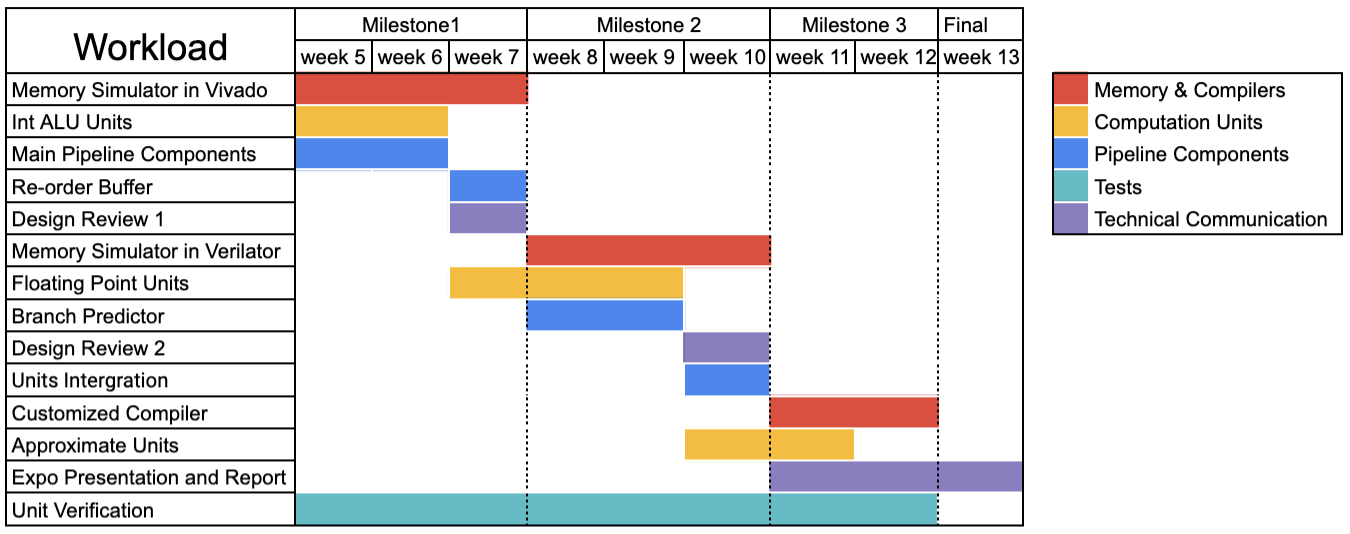
\includegraphics[width=0.8\linewidth]{figure/gantt.png}
    \caption{Project Gantt chart.}
    \label{gantt}
\end{figure}
Fig. \ref{gantt} shows a simplified Gantt chart of the project. The testing part should be conducted throughout the developing process. The rest four workloads will be distributed evenly into every milestone to make sure we can always balance our pace. 

From the chart we can observe that Week 2-5 is not included because what we have mainly done is preparation. We familiarize ourselves with the memory blocks on FPGA board and start to write main components in RISC-V out-of-order (O3) pipeline.
\begin{enumerate}
    \item By Milestone 1 (week 5 - week 7), we finished most parts of a naive RISC-V O3 core O3 such as Issue Queue, Reorder Buffer and Rename Table.
    \item By Milestone 1.5 (week 7 - week 8), we finished the simulation of a RISC-V O3 core to make sure the whole core runs without any syntax errors.
    \item By Milestone 2 (week 8 - week 10), we completed extra components like approximate units and customized compilers.
    \item By Milestone 3 (week 10 - week 12), we will have a complete flow to run an image processing C program on our synthesized RISC-V core.
\end{enumerate} 

We assign different workloads to different teammates based on their respective expertise. Jian Shi and Yichao Yuan will be in charge of memory related units. Yiqiu Sun will be responsible for computation unit. Li Shi and Zhiyuan Liu will be responsible for pipeline related units.
 
Our initial goal is to build our whole design on FPGA board. However, after synthesizing some part of our modules on Vivado, we found that our available FPGA board is inadequate to build such large circuits. There are too many unavoidable I/O ports in our design. Therefore, we have switched our plan to run software simulation of our design through Verilator. At this point, every workload can be done on software. In conclusion, the overall project is expected to be finished without any funding.


\section{Manufacturing Plan} %syq
The whole implementation involves different levels of the computer architecture hierarchy, with ranges from upper level compiler design to lower level circuit synthesis. Fig. \ref{fig:implement_plan} shows a flow chart of our manufacturing plan. 

\begin{figure}[!htp]
    \centering
    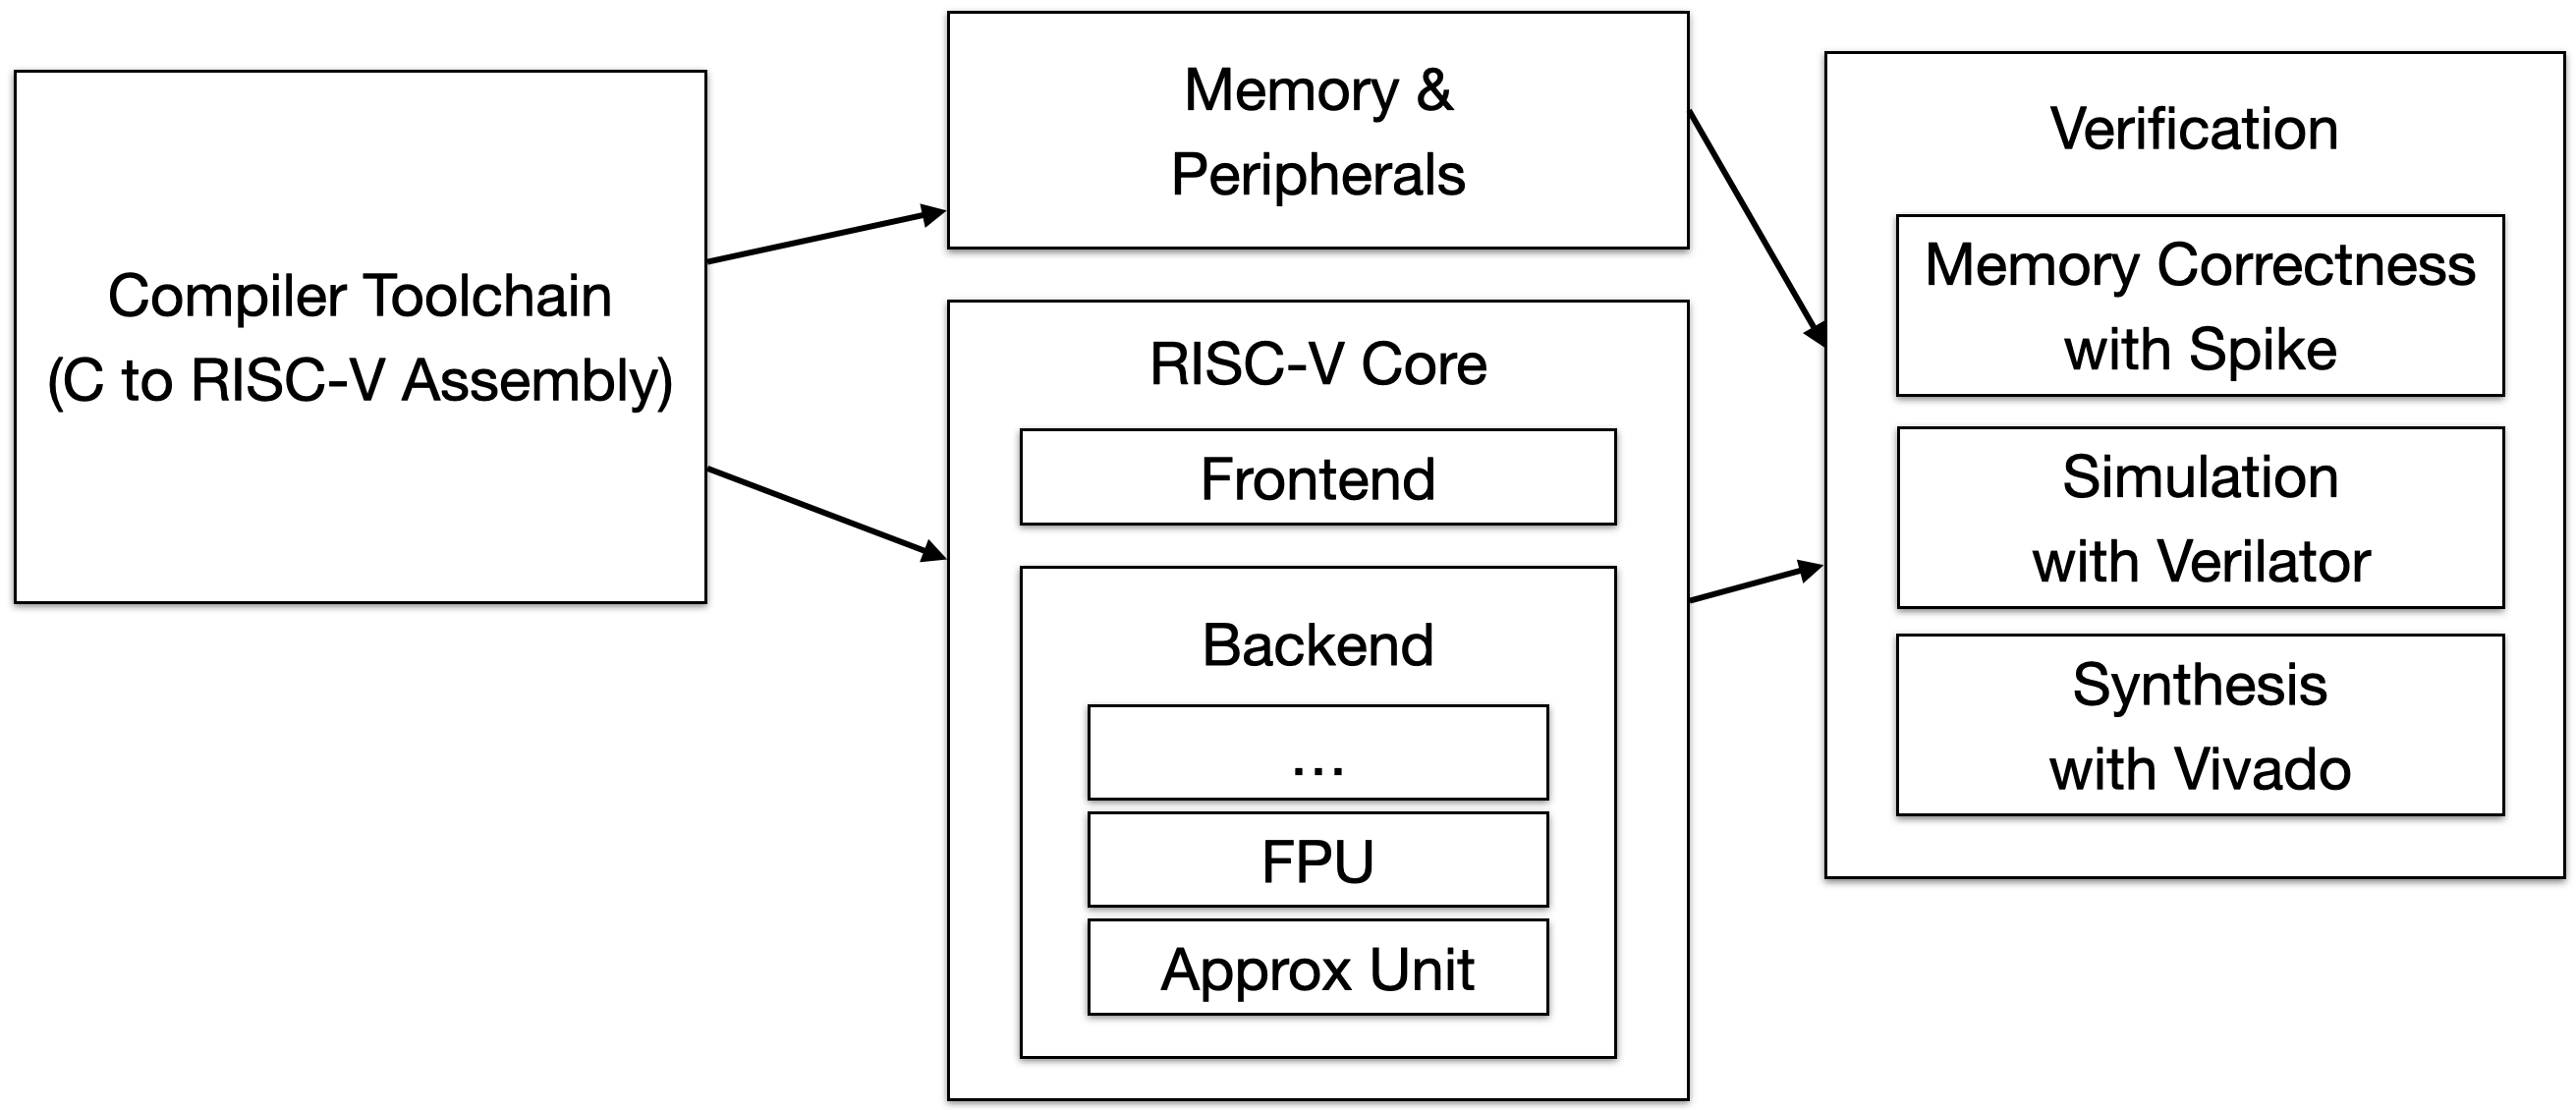
\includegraphics[width=0.6\textwidth]{figure/implement_plan.png}
    \caption{Manufacturing plan diagram.}
    \label{fig:implement_plan}
\end{figure}

To make our processor ``understand'' those operations assigned, we will first build a compiler to ``translate'' higher-level programming language like C language into assembly code, which is understandable by processor. Meanwhile, we also need to customize the compiler to translate floating point operation into approximate computing instead of accurate computing. The detailed implementation is explained in Section \ref{section:Customized Instructions}.

After the program is translated to assembly code, it is ready to be transported into the Memory and run on the RISC-V core that we are going to build. The Memory core is simulator of the DRAM, which is always on a separate chip other than the CPU chip in a real case. The RISC-V core will be written in System Verilog, which is hardware description language used to design and test electronic systems. The detailed design of our RISC-V core is demonstrated in Section \ref{section:Microarchitecture}. 

After finishing the Memory and RISC-V Core, we need to perform several level of verification towards our designed circuit because a functional-correct design might not be practical for real circuit synthesis. The whole verification includes memory correctness, simulation correctness and synthesis correctness. We uses tools such as Spike, Verilator and Vivado. The details will be discussed in \ref{section: Validation}.

\section{Validation} \label{section: Validation}
We introduce the validation part through a top-down approach: we will first introduce the software stack, then the simulator architecture. We validate our design by comparing the simulation of our CPU model and an golden RISC-V reference model, Spike. The software need to compile the source code into binary that can use the approximate computation units in the model as well as can run on these two target. 

\subsection{Program layout in memory} %yyc
We need a clear picture about how the program layouts in the simulator and Spike so that we can control the IO behavior of the program, like refering to where to fetch instructions, data and output result. The layout of the program and the physical address space of both the Spike is shown in the Fig.~\ref{fig:450-addr-sapce}. The left hand side shows how will the program be loaded into our verification environment. The \texttt{data} and \texttt{bss} segments are placed starting from 0x10000000 and the text segment is placed start from 0x80000000. The stack is set to start from 0x20000000, growing downwards. 

The right hand side is the devices related to the physical address in Spike. Our modified Spike as a DRAM device starting from 0x10000000, where all the segments and the stack will locate. There are some other devices with the Spike, like ROM, CLINT and MMIO. However, none of them will be used in this project so they will not be introduced. 

Our simulator using Verilator has an idea memory space, which means every physical address corresponding to a piece of memory, so there is no need to elaborate here. 

\begin{figure}[!htp]
    \centering
    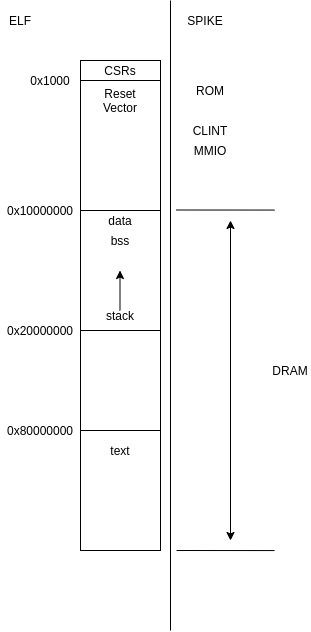
\includegraphics[width=0.35\textwidth]{figure/450-mem.png}
    \caption{Address space configuration in ELF format and Spike simulator.}
    \label{fig:450-addr-sapce}
\end{figure}

\subsection{IO libraries} %yyc
On a normal Linux machine, some special operations like opening a file and printing a string requires system calls. Similarly, in both our simulator and Spike, the running program performs such operations through special methods. We provide several function to encapsulate the IO operations. The implementation of the library has a lot to do with the Spike architecture and the simulator's architecture, so it will be introduced later. Following is a list of functions we provided.

\begin{enumerate}
    \item \texttt{tohost\_exit()} function takes an integer as the exit code and terminate the simulation.
    \item \texttt{tohost\_printstr()} function takes a pointer to string to print a string.
    \item \texttt{tohost\_open()} takes the filename and flags as argument, and return a file descriptor
    \item \texttt{tohost\_close() }takes a file descriptor as an argument. It close the corresponding file.
    \item \texttt{tohost\_write()} takes a file descriptor, a pointer to buffer and a length to write data to the file.
    \item \texttt{tohost\_read()} takes a file descriptor, a pointer to buffer and a length to read data from the file to the buffer.
\end{enumerate}

These functions like the system call in system programming. The function setup the register properly using the convention with the front-end server. The algorithms can use \texttt{tohost\_open()}, \texttt{tohost\_close()}, \texttt{tohost\_write()} and \texttt{tohost\_read()} to do IO with a file. For example, an imaging program can open a file to read the inputs and write the output to a file. The print function can be used to debug.

\subsection{Compilation Toolchains} %lzy
We also need to modify the compilation toolchains accordingly, so that the compiler can issue and disassemble our customized instructions. RISC-V has its own compilation toolchains and provides multiple types of cross-compilers listed below 
\begin{itemize}
    \item riscv32/64-unknown-elf-gcc
    \item riscv32/64-unknown-linux-gnu-gcc
    \item riscv64-multilib-elf-gcc
    \item riscv64-linux-multilib-elf-gcc
    \item riscv-none-embed-gcc
\end{itemize}

The suffix \texttt{32} and \texttt{64} points out whether to support 32 bits RISC-V architecture or 64 bits RISC-V architecture while the cross-compiler with the \texttt{multilib} suffix can support both architectures at the same time. The cross-compiler with the \texttt{linux} suffix uses \texttt{glibc} a dynamic link library, as C runtime library, while the one without the \texttt{linux} suffix uses the static link library \texttt{newlib} as C runtime library. The last cross-compiler is designed for bare-metal embedded system. 

In our project, we propose a SOC design targeted for embedded system. For embedded system, we should use the static link library (\texttt{newlib}) as C runtime library. Our project only supports 32 bits RISC-V architecture now, but in order to be better compatible with 64 bits architecture in the future, we choose the \texttt{multilib} cross-compiler.  In summary, we choose \texttt{riscv64-multilib-elf-gcc} as our target cross-compiler and modify it to support our customized instructions. 

We also need to use \texttt{riscv-opcodes} tool to get the mask and match of our customized instructions. Our cross-compiler will use the mask and match to identify our customized instructions. Take \texttt{FMULA.S} as an example, by parsing opcodes, we can get \texttt{\#define MATCH\_FMULA\_S 0x30000053}, \texttt{\# define MASK\_FMULA\_S 0xfe00007f}. After changing the corresponding files in \texttt{riscv-binutils} and \texttt{riscv-gdb}, our cross-compiler can support the assembly and disassembly of customized instructions at the same time and our customized instructions can be called through C inline assembly.

% compilation flow (yyc)
The compilation is managed by make. The whole compilation is processed by parts. The whole process is demonstrated in the Fig.~\ref{fig:compilation}.


The library includes the startup code and the IO libraries, they are compiled in advanced to be object code. Since we do not have an OS environment, we cannot use the default startup code, so we write the startup code using assembly, which does nothing more than setup the stack and jump to the \texttt{main} function. The IO libraries provides method to open files, write files, etc.  The program sources are written in C and they are compiled into object files for link. We use our only link script to control the program layout. The text segments are place starting from 0x80000000 and the data segments, including sections like \texttt{.data}, \texttt{.bss}, etc., are place starting from 0x10000000. The linker will then output an ELF file for execution.

\begin{figure}[!htp]
    \centering
    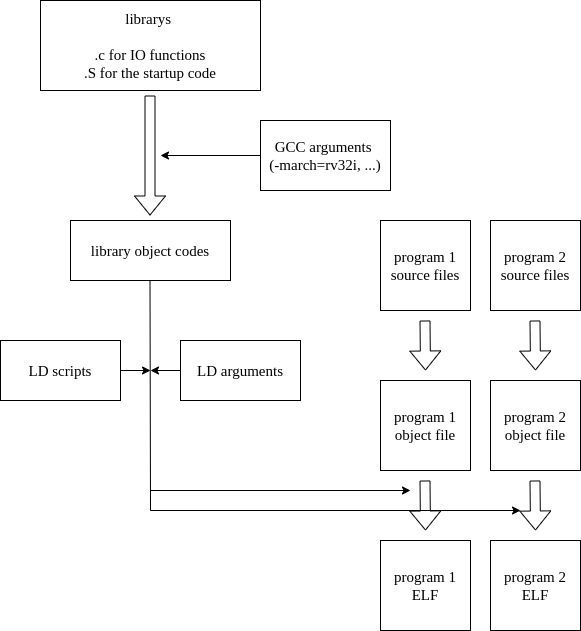
\includegraphics[width=0.7\textwidth]{figure/compilation.png}
    \caption{Compilation toolchains setup.}
    \label{fig:compilation}
\end{figure}

\subsection{Cycle-Accurate Verification Tool: Verilator} %yyc

Verilator is a program which can turn the Verilog and SystemVerilog HDL models in the C++ libraries. The results are some \texttt{.cpp} and \texttt{.h} files, in which the HDL models become classes. This process is called ``verilating'' and the generated models are called ``verilated''. The generated files can then be linked to C++ simulation environment to perform simulation. User uses their own C++ ``wrapper'' files, which instantiate the generated models. By setting values to the variables that corresponding to the signals in the HDL model, the simulation is performed. During the simulation, Verilator can generated useful information like log files as well as waveform. The whole program is compiled by a normal C++ compiler and becomes an executable. The user execute the executable to start the simulation. We use Verilator to perform logic simulation. The signals information is printed and waveform is dumped. We use those information to check the correctness of our model as well as do the HDL model meets our timing requirement.

The Verilator C++ wrapper file is integrated into the whole verification system. The verilated CPU model will have access to an ideal memory modeled by C++. The verification system will load the program into the idea memory based on the information in the ELF file. The wrapper file will also take the responsibility to handle IO operation like print and save files.

The detailed architecture of this verification environment is illustrated in Figure \ref{fig:ve-vm}. 

\begin{figure}[!htp]
    \centering
    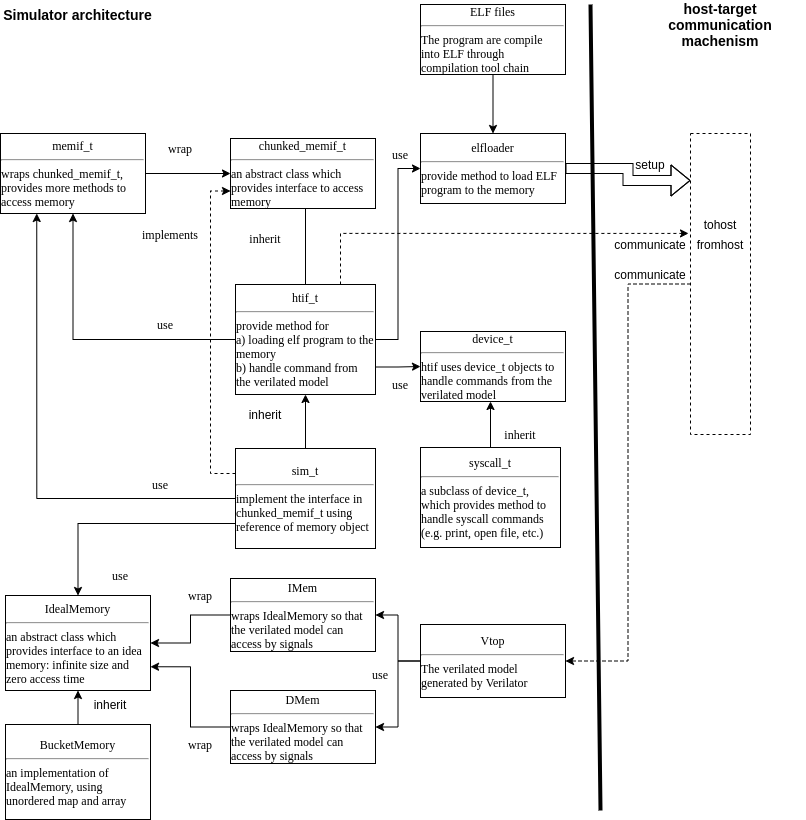
\includegraphics[width=\textwidth]{figure/simulator-archiecture.png}
    \caption{Verification environment based on Verilated model}
    \label{fig:ve-vm}
\end{figure}

This architecture reuse codes from the Spike simulator. The \texttt{chunked\_mem\_if} is an abstract class that provides interface to access the memory by other components in the simulator. The \texttt{mem\_if} class is a wrapper for the \texttt{chunked\_mem\_if}, which gives more convenient interfaces to access the memory. The \texttt{htif\_if} inherits from the \texttt{chunked\_mem\_if} class, which provides the methods to load the ELF files into the memory and handle communication with the running software. The \texttt{sim\_t} inherits from \texttt{htif\_if}, which use the reference to an object of \texttt{IdeaMemory} to implements the interface in \texttt{chunked\_mem\_if}. The \texttt{IdeaMemory} class is an abstract class, which is implemented by \texttt{BucketMemory}. The Verilated model uses two wrappers, \texttt{DMem} and \texttt{IMem}, to access the memory. They provide convenient interfaces for the Verilated Model. 

The Verilated Model, or more precisely the running program on the verilated model, communicate with each other through two variables in the memory, \texttt{tohost} and \texttt{fromhost}. These two variable should be defined in the program and they will have records in the ELF file. When the \texttt{htif\_t} loads the program, it will track the position of these two variables. The Verialted Model can write a value, which is called a command, in the \texttt{tohost} variable. The \texttt{htif\_t} will monitor the variable and process the command using \texttt{device\_t} classes. The result will be write in the \texttt{fromhost} valuable. The software can wait on the \texttt{fromhost} variable to finish the communication.

\subsection{Trace-Accurate Verification Tool: Spike} %yyc & lzy

Spike is a ``golden'' model of RISC-V which provides a trace-accurate model for the RISC-V specification. By using Spike, we can know the exact behavior of the correct processor. By comparing the result of the spike and the instruction retired from our Verilator model. If they are identical, then we can be sure we implement the specification correctly.

The front-end architecture, the way it loads program and handle the communication between target, has been introduced in the previous section because we build our verilator's environemnt using Spike's architecture.

% https://github.com/riscv/riscv-isa-sim/issues/364
The original Spike (v1.0.0) has limited IO support for \texttt{XLEN = 32} RISC-V architecture. Under the RV64 architecture, it is possible to use the spike's hardware-target interface to print characters on the screen by setting the command's device to 1. However, this interface is based on a 64 bit register. Under the RV32 architecture, there is no way to do atomic 64 bits write so the high 32 bits will always be 0. As a result, we will have no access to the device to print.

In this project, we proposed an additional system call \texttt{sys\_printstr} which use the same system call procedure to evoke like any other system call in spike. The new system call occupies the number 2012 and takes the pointer to string as an argument. This system call will print the string onto the standard output.

Another change we made on the original spike is change it memory mapping. the original memory map maps the DRAM to start from 0x80000000, which limits the way we write the linker script. We changed the memory mapping so that most of the physical memory has a meaning.

%spike - customized instruction (lzy)
To compare the result of the spike and the instruction retired from our Verilator model, spike should also support our customized instruction. For more information about our customized instructions, please refer to section \ref{section:Customized Instructions}. We use approximate computation algorithm written in C language to describe the functional behaviour of our customized instructions so that spike can simulate the floating-point approximate computing units in our design. 


\subsection{Validation of Engineering Specifications}
During the whole validation process, most of our engineering specifications will be tested. Part of engineering specifications require advanced test methods or more general tests and the overall validation results will be demonstrated in the final report.

\begin{table}[!htp]
    \centering
    \resizebox{\textwidth}{!} {
    \begin{tabular}{lcccc}
        \hline
        \textbf{Engineering Specification} & \textbf{Unit} & \textbf{Target} & \textbf{Actual} & \textbf{Comment} \\
        \hline
        Support RV32G instruction set architecture (ISA) & -     & Yes              & \textcolor{red}{Partial}  & RV32IM            \\
        Core frequency on FPGA test platform             & MHz   & 100 $\uparrow$   & \textcolor{red}{74.88}    & Synthesis result  \\ 
        Number of pipeline stages                        & -     & 9                & 9                         &                   \\
        Instructions executed per clock cycle (IPC)      & -     & 0.5 $\uparrow$   & \textcolor{red}{-}        & Under testing     \\
        Support instruction dynamic scheduling           & -     & Yes              & Yes                       &                   \\
        Typical total cache size                         & KB    & 32 $\uparrow$    & \textcolor{red}{0}        & Under development \\
        Number of function units                         & -     & 6 $\uparrow$     & 6                         &                   \\
        Average response time to a request for service   & ms    & 10 $\downarrow$  & \textcolor{red}{-}        & Under testing     \\
        Usage of look-up tables (LUT) on FPGA            & k     & 120 $\downarrow$ & 74.72                     & Synthesis result  \\
        Usage of block RAM (BRAM) on FPGA                & -     & 50 $\downarrow$  & 0                         & Synthesis result  \\
        Usage of digital signal processor (DSP) on FPGA  & -     & 30 $\downarrow$  & 8                         & Synthesis result  \\
        Power consumption on target FPGA test platform   & W     & 5 $\downarrow$   & \textcolor{red}{-}        & Under testing     \\
        Operations processed within unit energy.         & MOp/J & 25 $\uparrow$    & \textcolor{red}{-}        & Under testing     \\
        Number of flexibly-configured modules            & -     & 10 $\uparrow$    & 13                        &                   \\
        Number of I/O device types                       & -     & 3 $\uparrow$     & \textcolor{red}{0}        & Under development \\
        User guide and programmers manual                & -     & Yes              & Yes                       &                   \\
    \hline
    \end{tabular}
    }
    \caption{Engineering specification validation ($\uparrow$ high is better / $\downarrow$ lower is better).}
    \label{es-validation}
\end{table}

Part of engineering specifications can be validated manually by checking the source code of the RTL design model or the corresponding supplementary materials of our processor:

\begin{enumerate}
    \item Number of pipeline stages: We check the original design diagram of our processor (Fig.~\ref{fig:pipeline}) and count the number of pipeline stages.
    \item Number of function units: We check the design and count the number of function units.
    \item Number of flexibly-configured modules: We check the source code and count the number of flexibly-configured modules, including fetch buffer, register renaming unit, issue units, etc.
    \item User guide and programmers' manual: We check the manual supplementary materials of our processor.
\end{enumerate}

Part of engineering specifications can be validated by software validation tools, including Verilator and Spike:

\begin{enumerate}
    \item Support RV32G instruction set architecture (ISA): We cross-compile C programs into binaries compatible with RV32G ISA and run on our processor.
    \item Instructions executed per clock cycle (IPC): We run benchmark programs on our processor and acquire the data of both number of instructions and clock cycles to execute the programs. We then derive the average value of IPC of our processor.
    \item Support instruction dynamic scheduling: We check Verilator simulation logs and prove that instruction dynamic scheduling algorithm works well.
    \item Typical total cache size: We manually set the cache size in Verilator simulation model.
    \item Average response time to a request for service: We count the clock cycles of some response programs. Based on core frequency on FPGA test platform, we then derive the average response time.
    \item Number of I/O device types: We count the virtual I/O devices in our software model.
\end{enumerate}

Part of engineering specifications can be validated by Xilinx Vivado EDA tool:

\begin{enumerate}
    \item Core frequency on FPGA test platform: During the process of synthesis and implementation, Vivado performs static timing analysis (STA) on our RTL model and gives the data of critical delay in nanosecond. We then derive the core frequency of our processor on FPGA test platform.
    \item Usage of look-up tables (LUT), block RAM (BRAM) and digital signal processor (DSP) on FPGA: We check Vivado synthesis report and acquire related data of resource usage on FPGA platform.
    \item Power consumption on target FPGA test platform: We check Vivado synthesis and implementation report and acquire the dynamic power of our design.
    \item Operations processed within unit energy: Based on specific benchmark programs, the value of core frequency and power consumption, we estimate the value of operations processed within unit energy.
\end{enumerate}
% isn't this the validation result?

The correctness of the CPU is validated using the test suit describe above. We performed the test on
\begin{enumerate}
    \item a simple program written in assembly to test whether the CPU can correctly conduct simple instructions like arithmetic, jump, branching etc
    \item some simple C programs which do not include any system calls. These program are test to check whether the CPU can run simplest real program as well as whether the whole validation flow works correctly.
    \item some C programs that can do real works using system call. A image processing program is compiled and tested.
\end{enumerate}

%\section{Validation Result} \label{section: Validation Result}
%The design uses
% = = = = = = = = = = = = = = = = = = = = = %
%               Discussion                  %
% = = = = = = = = = = = = = = = = = = = = = %

\let\clearpage\relax

\chapter{Discussion \& Future Work} %syq

\section{Load-Store Unit}
\subsection{Problem}
The most significant characteristic of an out-of-order core is that the order of executed instructions is random, including memory access instructions. With the help of ROB, we can ensure that the results of all the integer and floating point instructions are correct. However, without specifically designed load-store unit, we cannot ensure that the content in the memory is consistent. For example, consider the following two instructions.
\begin{equation*}
    \centering
    \texttt{sw x1, 0(x2); lw x3, 0(x4)}
\end{equation*}
If the addresses stored in \texttt{x2} and \texttt{x4} are identical, there exists potential memory data dependency, i.e., memory alias, under which circumstance the two instructions must be executed sequentially. Thus, we need a load-store unit to ensure that the memory consistency is kept. As mentioned in the issue logic for memory access instructions, currently our strategy is to consider all store instructions as barriers, i.e., we don't care the order of load instructions between two store instructions, but the store instructions must be executed sequentially.

However, we still need to consider the case of branch mis-prediction. If a branch mis-prediction occurs, speculative load instructions will not influence the memory consistency, but speculative store instructions will. For example, a store instruction following a branch mis-prediction will write the wrong value to the memory, which is irrevocable.

\subsection{Current Solution \& Future Work}
To resolve this conflict, a load-store unit is necessary to keep memory consistency. Currently we design a simple store buffer simulated in Verilator. As it is implemented in software, there is no limitation in terms of size and delay. When speculative store instructions are executed in the execution stage, the processor will send a store request to the store buffer. Only when these store instructions commit, the store buffer will write the data to corresponding memory addresses. If a branch mis-prediction occurs and sends a recover signal, the content of store buffer will be immediately flushed. Furthermore, when load instructions are executed, we will first check whether there exists store instructions that share the same address with load instructions. If so, we directly return the data from store buffer. Otherwise, we load the data from main memory as usual. Fig.~\ref{fig:store-buffer} shows a simplified diagram of store buffer in our memory access system.

\begin{figure}[!htp]
    \centering
    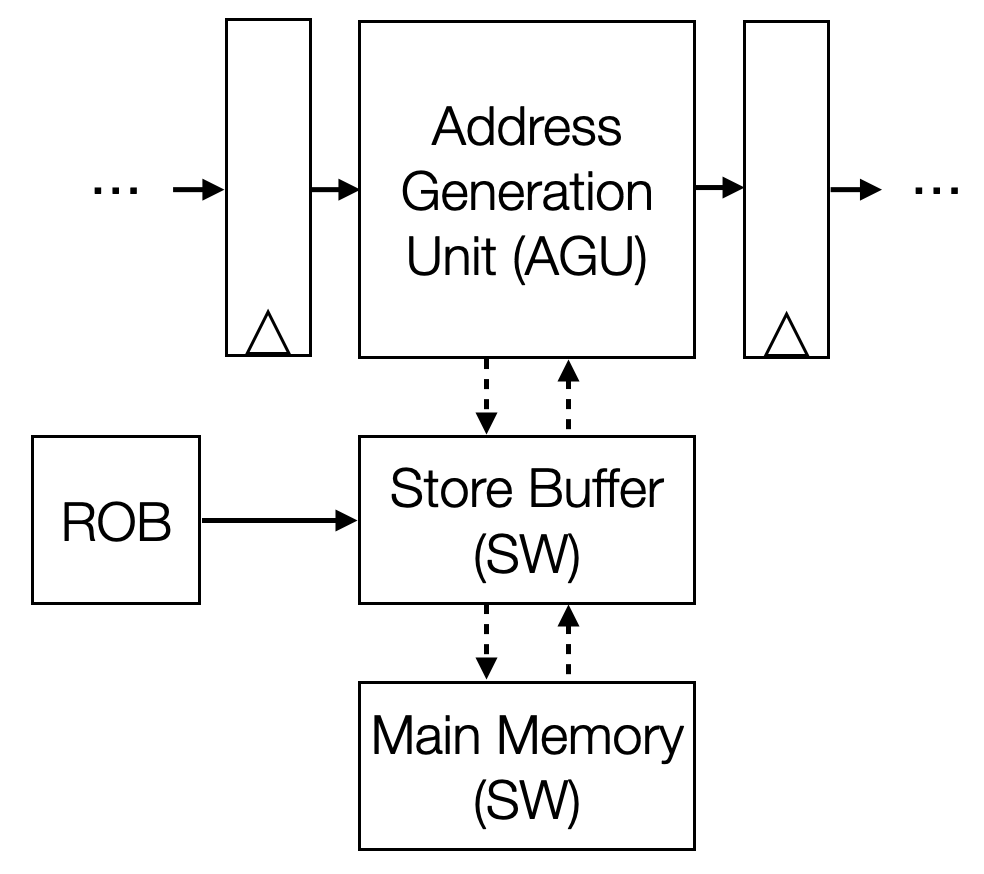
\includegraphics[width=0.4\textwidth]{figure/store_buffer.png}
    \caption{Current solution of store buffer.}
    \label{fig:store-buffer}
\end{figure}

In the future, we may implement the store buffer in RTL design. We may also further improve the performance of memory access by introducing more complicated load-store unit, e.g., miss status handling register (MSHR).


\section{Pipeline Optimization}
\subsection{Problem}

We designed our Out-of-order ten-stage processor based on several designs such as the "BOOM" design mentioned in section \ref{section: BOOM}. However, there are still some room for optimizations in mircoarchitectures. Two stages that perform independent operations can be combined. The stage that takes longer time than others should be split to shorten the critical path.

For example, the decoding and renaming are separated into two stages currently. This means we have to wait for at least two cycles to dispatch decoded instructions (one in Rename stage, one in Dispatch stage). In addition, in the issue stage, we can only figure out the physical register number needed, instead of the actual value. And we have wait another cycle to read the value from the physical register file in the Registerfile (RF) stage. The same problem applies to the Writeback and Commit stages. After an instruction finishes execution, it will first write back its calculated value. We have to wait at least one more cycle to commit this instruction.

Meanwhile, the Dispatch stage can be split. The Reorder Buffer in this stage can remain the same while the dispatch can be combined to the following Issue stage.


\begin{figure}[!htp]
    \centering
    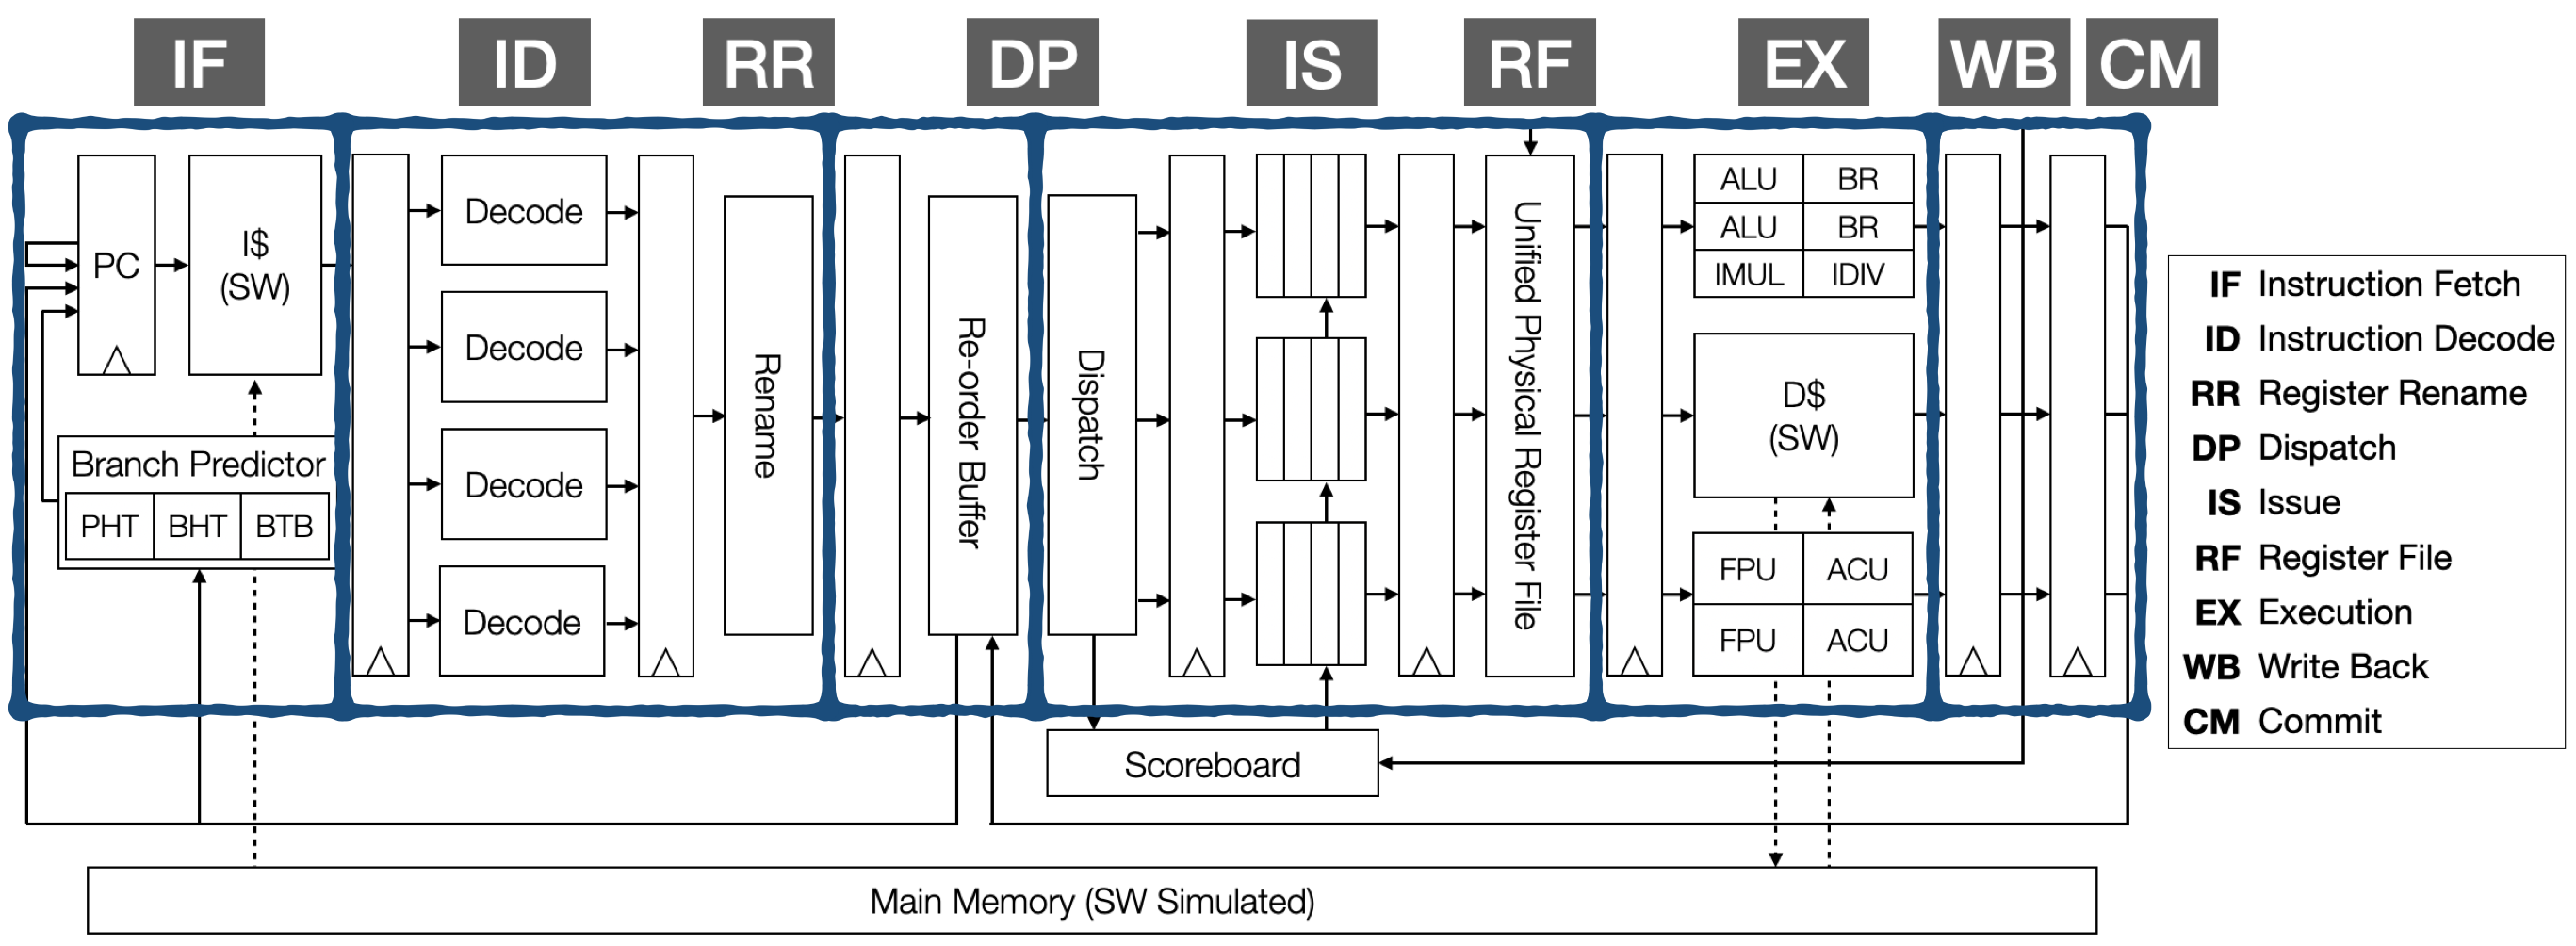
\includegraphics[width=\textwidth]{figure/new_design.png}
    \caption{Optimized RISV-V core design draft}
    \label{fig:opt_core}
\end{figure}

\subsection{Current Solution \& Future Work}
According our discussion in the above Problem section, the possible optimized stage distribution is shown in Fig. \ref{fig:opt_core}. Since it is just an optimization, it won't affect the correctness of the current design. Our current design is still runnable and functionally correct. In the future, we will apply those optimizations and analyze the performance gained from the changes.
% = = = = = = = = = = = = = = = = = = = = = %
%                 Conclusion                %
% = = = = = = = = = = = = = = = = = = = = = %

\let\clearpage\relax
\chapter{Conclusion}

In this project, we design a processor based on RISC-V ISA and simulate the SoC with software tools. Our processor supports 4-way superscalar execution and instruction dynamic scheduling, which keeps a good performance-energy-cost balance and involves complex algorithm and logic design. As the project is mainly for research and education purpose, it offers users a good base to explore computer architecture design and optimization.


}

%TC:ignore

% 致谢
% !TEX root = ../main.tex

\begin{acknowledgements}

Throughout the capstone design project of ``RISC-V SoC Microarchitecture Design and optimization'', we have received a great deal of support and assistance.

We greatly appreciate our instructor, Dr. Weikang Qian from UM-SJTU Joint Institute at Shanghai Jiao Tong University. As the instructor of our project, he listens to our weekly report and gives many constructive suggestions. Besides, he provides much support for us, not only in the technical part, but also in terms of our future career planning, etc. His insightful feedback pushes us to sharpen our thinking and brings our work to a higher level.

We greatly thank Dr. Jigang Wu, Dr. Chengbin Ma, Dr. Peisen Huang, Dr. Gang Zheng, Dr. An Zou and Dr. Mingjian Li from UM-SJTU Joint Institute at Shanghai Jiao Tong University, who are the course instructors of \textit{VE450 Major Design Experience} at Joint Institute. We also greatly thank the whole teaching assistant team of this course. They teach us many concepts of engineering design process and project management, which helps us explore from the engineering problems and needs to the concept selection and final solutions.

In addition, we would like to express our greatest gratitude to our parents. No matter what kind of difficulties we are facing, they are always there, providing firm and unconditional support for us. We would like to thank our friends and schoolmates at Joint Institute for their personal support in our academic endeavours during the past four years.

Thanks to \href{https://github.com/sjtug/SJTUThesis}{\sjtuthesis~Team} for providing the \LaTeX~template for this thesis document.

\end{acknowledgements}


% 附录
\appendix
{
\setstretch{1.5}
\setlength{\parindent}{0pt}
\setlength{\parskip}{1em}
% \renewcommand{\thechapter}{\Roman{chapter}}
\captionsetup{list=no}

% = = = = = = = = = = = = = = = = = = = = = %
%                  Appendix                 %
% = = = = = = = = = = = = = = = = = = = = = %

% = = = = = = = = = = = = = = = = = = = = = %
%                    Bios                   %
% = = = = = = = = = = = = = = = = = = = = = %

\chapter{Bios}

\section{Li Shi}

\begin{minipage}{0.25\textwidth}
  
\includegraphics[width=1.2in,height=1.5in,clip,keepaspectratio]{figure/sl.png}
\end{minipage}
\begin{minipage}{0.75\textwidth}\raggedright
  \begin{tabular}{l l}
    \textbf{Major}          & Electrical \& Computer Engineering \\
    \textbf{Student ID}     & 517370910032 \\
    \textbf{SJTU Email}     & \url{shili2017@sjtu.edu.cn} \\
    \textbf{Personal Email} & \url{shili2048@gmail.com} \\
    \textbf{Phone}          & +86-14782059981
  \end{tabular}
\end{minipage}

I am Li Shi, a senior undergraduate major in ECE at JI. I like studying photography, watching sci-fi movies, eating Chinese food (especially Sichuan cuisine), and sleeping. Also, I enjoy playing with kittens and puppies.

Before the capstone design project, I have been working on the High-Level Synthesis project instructed by Prof. Weikang Qian at JI for about 2 years, during which I accumulated some experience on digital design, software engineering, compiler design, etc. Meanwhile, I once worked as an intern at Apple, where I participated in developing a CPU simulator and studied computer architecture by myself. My interests include digital design, embedded systems, computer architecture, etc. In 2022, I will start my journey in M.S. in ECE program at Carnegie Mellon University.


\section{Zhiyuan Liu}

\begin{minipage}{0.25\textwidth}
  \includegraphics[width=1.2in,height=1.5in,clip,keepaspectratio]{figure/lzy.png}
\end{minipage}
\begin{minipage}{0.75\textwidth}\raggedright
  \begin{tabular}{l l}
    \textbf{Major}          & Electrical \& Computer Engineering \\
    \textbf{Student ID}     & 517370910240 \\
    \textbf{SJTU Email}     & \url{angelinaliu@sjtu.edu.cn} \\
    \textbf{Personal Email} & \url{?} \\
    \textbf{Phone}          & +86-?
  \end{tabular}
\end{minipage}

My name is Zhiyuan Liu, a senior student in JI major in ECE. I like drawing, photography, playing video games, and basketball. Besides, I like to assemble computers by myself. Before the capstone design project, I studied VE270 Introduction to Logic Design and VE370 Intro to Computer Organization in JI, and I also learned VE470 Computer Architecture by myself. I am very interested in computer architecture. I once worked as an intern at Microsoft and I participated in feature development for products there.

This fall, I will become a regular employee of Microsoft.


\section{Yiqiu Sun}

\begin{minipage}{0.25\textwidth}
  
\includegraphics[width=1.2in,height=1.5in,clip,keepaspectratio]{figure/syq.jpeg}
\end{minipage}
\begin{minipage}{0.75\textwidth}\raggedright
  \begin{tabular}{l l}
    \textbf{Major}          & Electrical \& Computer Engineering \\
    \textbf{Student ID}     & 517370910020 \\
    \textbf{SJTU Email}     & \url{susansun@sjtu.edu.cn} \\
    \textbf{Personal Email} & \url{?} \\
    \textbf{Phone}          & +86-?
  \end{tabular}
\end{minipage}

My name is Yiqiu Sun. I major in ECE at JI and CE at University of Michigan. Interested in Computer Architecture and new computing techniques like approximate computing, I worked with Prof. John Hayes on stochastic computing and with Prof. Trevor Mudge on re-configurable accelerators. Meanwhile, my course experience of EECS 470 Computer Architecture at Michigan would help me better contribute to this project. This fall, I will pursue my Ph.D. degree in computer science in University of Illinois at Urbana-Champaign. With a research focus on In-Memory Computing, I would like to figure out a better communication scheme between processor and memory in the future.

Besides academics, I am interested in cooking and hiking. I also adopted two cats. They are Gomez and Kent. These two fluffy creatures are my best life companions.


\section{Jian Shi}

\begin{minipage}{0.25\textwidth}
  
\includegraphics[width=1.2in,height=1.5in,clip,keepaspectratio]{figure/sj.jpg}
\end{minipage}
\begin{minipage}{0.75\textwidth}\raggedright
  \begin{tabular}{l l}
    \textbf{Major}          & Electrical \& Computer Engineering \\
    \textbf{Student ID}     & 517370910255 \\
    \textbf{SJTU Email}     & \url{timeshi@sjtu.edu.cn} \\
    \textbf{Personal Email} & \url{?} \\
    \textbf{Phone}          & +86-?
  \end{tabular}
\end{minipage}

I am Jian Shi, a senior student major in ECE at JI. I like taking photos, analyzing video games and swimming. Also, I am a full stack developer. I build and maintain an online server by myself. Starting from choosing hardware components in the server, to the deamon service written by myself, I learn a lot from this experience. Currently, the server has become my computing center. Whenever I have a task that can be processed or maintained by computer or network, I will write a program and throw it to my server. By the way, the test platform for this project is also based on my server.

This fall, I will continue my Ph.D. degree at JI under Prof. Weikang Qian's guidance. I think this project will help a lot in my future Ph.D. study.


\section{Yichao Yuan}

\begin{minipage}{0.25\textwidth}
  
\includegraphics[width=1.2in,height=1.5in,clip,keepaspectratio]{figure/yyc.jpg}
\end{minipage}
\begin{minipage}{0.75\textwidth}\raggedright
  \begin{tabular}{l l}
    \textbf{Major}          & Electrical \& Computer Engineering \\
    \textbf{Student ID}     & 517370910233 \\
    \textbf{SJTU Email}     & \url{yyc19990826@sjtu.edu.cn} \\
    \textbf{Personal Email} & \url{?} \\
    \textbf{Phone}          & +86-?
  \end{tabular}
\end{minipage}

My name is Yichao Yuan. I am a senior student in JI major in ECE. I like movies, graphics and various technology topics. I enjoy writing software and building hardware and the beauty of their interaction always amazes me. Before the capstone project, I have solid knowledge at each abstraction layer of hardware. In JI, VE270 and VE370 introduce basics about logic design and computer organization. In 2020 spring, I took CS152 and EECS151 in UC, Berkeley, which gave me advanced knowledge in computing architecture and digital design.

This fall, I will be an ECE M.S. student at University of Michigan, Ann Arbor.

% % = = = = = = = = = = = = = = = = = = = = = %
%                 Conclusion                %
% = = = = = = = = = = = = = = = = = = = = = %

\let\clearpage\relax
\chapter{Discussions and Conclusion}

\blindtext

\section{Figures}

\subsection{Single Figure}

\begin{figure}[!htp]
    \centering
    \includegraphics[scale=0.5]{example-image-a}
    \caption{Figure-A.}
    \label{fig:a}
\end{figure}

\subsection{Subfigures}

\begin{figure}[!htp]
    \begin{minipage}{0.48\textwidth}
        \centering
        % include first image
        \includegraphics[scale=0.5]{example-image-a}
        \caption{Subfigure-A.}
        \label{fig:sub_a}
    \end{minipage}\hfill
    \begin{minipage}{0.48\textwidth}
        \centering
        % include second image
        \includegraphics[scale=0.5]{example-image-b}
        \caption{Subfigure-B.}
        \label{fig:sub_b}
    \end{minipage}
\end{figure}

\section{Table}

\begin{table}[!htp]
    \begin{center}
    \caption{Table-1.}
    \label{tab:tab-1}
        \begin{tabular}{cc}
            \toprule
                Item   &   Value \\
            \midrule
                A      &   1,000 \\
                B      &   2,000 \\
                C      &   3,000 \\
            \bottomrule
        \end{tabular}
    \end{center}
\end{table}

\section{Citation}

Single document with available page number~\quickcite{kopka1995guide}.

Single document without available page number~\quickcitenopage{kottwitz2015latex}.

Two documents at the same time~\quickcitetwo{lamport1985i1}{kopka1995guide}.

\section{Source Code}

\subsection{Pseudocode}
\begin{algorithm}
\caption{Algorithm 1.}
\label{alg:alg-1}
    \KwIn{integers $a,b$}
    \KwOut{integers $c$}
    \If {$a > b$} {
        $c = a - b$ \;
        \tcp{This is a comment.}
    }
    \Else {
        $c = a + b$ \;
    }
\end{algorithm}


}

% 结尾部分
\backmatter

% 参考文献
\printbibliography[heading=bibintoc]

% 个人工作报告
{
\setstretch{1.5}
\setlength{\parindent}{0pt}
\setlength{\parskip}{1em}

% = = = = = = = = = = = = = = = = = = = = = %
%                Individual                 %
% = = = = = = = = = = = = = = = = = = = = = %


\includepdf{scans/report-cover.pdf}
\addcontentsline{toc}{chapter}{Individual Contribution Reports}
\chapter*{Li Shi's Individual Contribution Report}

In our capstone design of ``RISC-V SoC Microarchitecture Design and Optimization'', based on RISC-V instructions set architecture (ISA), we design a processor, apply some advanced optimizations, and set up the SoC in software simulator tools. During this process, each team members contribute to the processor design and optimization.

To design a processor based on RISC-V ISA requires the efforts from not only the hardware part, but also from the software part. In our team, Jian Shi, Yiqiu Sun and I are hardware engineers, while Yichao Yuan and Zhiyuan Liu are software engineers. We hold the group meetings twice a week and co-design the hardware circuit design and software debugging workflow to build our RISC-V processor. Each member contributes to the processor design equally, and here is each member’s contribution to the project.

\begin{enumerate}
  \item Jian Shi is responsible for designing the hardware frontend, including register renaming table, free list, re-order buffer. He also designs the floating-point units in the execution units in the backend. Besides, during the preparation stage of this project, he is partially responsible for the survey of open-source RISC-V core and SoC and reads some academic articles. His workload is about 15 hours per week.
  \item Yiqiu Sun is responsible for designing and integrating the overall microarchitecture. She provides technical support for the team and designs the instruction fetch unit and branch predictor. Meanwhile, she helps other team members review the code, raises many constructive suggestions, and improves the overall design quality. Her workload is about 15 hours per week.
  \item Yichao Yuan is responsible for software simulation and validation. He helps the team to validate the processor design in software design tools, including Xilinx Vivado, Verilator, Spike, etc. Besides, although not implemented in the final design, he explores the instruction and data cache design and AXI bus protocol for the SoC. His workload is about 15 hours per week.
  \item Zhiyuan Liu is responsible for compilation workflow. She builds and modifies compiler toolchains, which is important for embedded system construction. She also adds our custom RISC-V instructions for approximate computing to the compiler so that users can use these custom instructions in their C programs. Her workload is about 15 hours per week.
  \item I am responsible for hardware backend design, including instruction dispatch, issue units, scoreboard, physical register file and part of execution units. At the same time, I also participate in integrating the microarchitecture and debugging. My workload is about 15 hours per week.
\end{enumerate}

As mentioned in the previous part, I am the hardware engineer in our team, and my job is mainly concentrated on register transfer level (RTL) design and optimization. 

In terms of the technical part, it is my second time to design a CPU core with hardware design language, and it is also the first time that I participate in designing a large processor core that supports superscalar execution and instruction dynamic scheduling. During this process, I have learned many basic concepts in computer architecture, digital design, and embedded systems. During the preparation stage, I investigate many open-source RISC-V cores and compare them in terms of performance, cost, and energy efficiency. After the project starts, I deep dive into the hardware design part. 

The microarchitecture design part is one of the core parts in our project and requires many concept selections and trade-off in the detailed designs. For example, in terms of the design of instruction dispatch stage, we have two options: collapsing-style dispatch and non-collapsing-style dispatch. The former means that we need to compress the incoming instructions and send to the issue stage, while the latter just selects the instructions and marks the unnecessary instruction as invalid. After carefully comparing the two design styles, I choose to implement the first one, which is more complicated, but can reduce the logic complexity in the issue stage. Later in the issue and register file stage, we also have two options: whether we should first read from the register file and then pass the values to the issue stage, or first issue the instructions and then read from the register file. The former may lead to higher efficiency, but we need to store all the source operand values in the issue units and frequently pass these values. On the contrary, the latter can save such unnecessary operations, save some power, and fits the customer requirements in embedded systems. Thus, after this process of analysis and referring to other open-source RISC-V cores, I choose to implement the latter design. We need to carefully compare the designs and choose the best fit for our processor.

In terms of the engineering project management part, I also learn a lot during the process of this capstone project. We apply many useful project management tools, including Feishu docs, which is useful to draw Gantt chart and track each group member’s schedule, and Git, which helps the team to manage the project repository as well as review the source code. For example, in the Feishu docs page of ``VE450 project management'', I record my progress and plan on a weekly basis, which will be automatically shown in the generated Gantt chart. In the group meeting, I report my weekly progress and share my hardware design or workflow with my team members. In the Git repository, I create my own working branches, including \texttt{Li/IssueQueue}, \texttt{Li/Dispatch}, \texttt{Li/ExecutionUnit}, etc., so that other people can easily check my progress and personal contribution to the project.

In terms of the technical communication part, I actively participate in the preparation for each design review and final expo. In design review 1, I am responsible for present our customer requirements and engineering specifications. In design review 2, I demonstrate our first version of processor design. In design review 3, I present our final microarchitecture design which consists of 9 pipeline stages in the frontend and backend. In the final expo, I participate in the oral defense and JI design expo. I try my best to not only work hard on the project itself, but also present our project to the audience so that people can clearly understand what we have done and how they can utilize our processor to do great things.

In brief, as one of the hardware engineers in the team, I actively contribute to the project of ``RISC-V SoC Microarchitecture Design and Optimization''. We work as a team and design a complicated RISC-V processor.


\includepdf{scans/report-cover.pdf}
\chapter*{Zhiyuan Liu's Individual Contribution Report}

Our capstone design topic is ``RISC-V SoC Microarchitecture Design and Optimization'' and in this project, we propose a processor design that can support 4-way superscalar execution and instruction dynamic scheduling together with some advanced optimizations like approximate floating-point computing units to solve challenges in AI-oriented embedded system which requires the CPU to be energy-efficient, inexpensive and fast at same time. After designing our processor, we also set up the SoC and peripheral components like cache and I/O devices in software simulator tools to test and validate our design. Our project can be divided into hardware part and software part. Li Shi, Jian Shi and Yiqiu Sun are mainly hardware engineers in our team while Yichao Yuan and I are software engineers. We hold our group meetings two to three times a week and there are also some individual meetings. Besides, we have meetings with our instructor every two weeks to report our project progress and explain some technical issues. Everyone has done their best for our design and everyone has contributed to our project equally, the following is our division of work.

\begin{enumerate}
  \item Li Shi: He is responsible for most of backend designs like instruction dispatch, instruction issue, register file and execution units for integer and memory access. He also helps debug and integrate FP components. His workload is about 15 hours per week.
  \item Jian Shi: He is responsible for hardware frontend designs such as free list, register renaming table, reorder buffer and execution units for floating point. At the same time, during the preparation phase of our project, he also did a lot of research on other RISC-V cores. His workload is about 15 hours per week.
  \item Yiqiu Sun: She is responsible for designing the branch predictor and instruction fetch unit and helps integrate and design our overall microarchitecture. She is also our technical support and helps review our code and proposes many constructive ideas about our design. Her workload is about 15 hours per week.
  \item Yichao Yuan: He is responsible for software simulation and validation part. He helps to replicate the Spike-based model to our verilator-based model, so that our CPU core can be better compared with the Spike model, and help simulation and validation. He also explores cache design and AXI bus protocol for our project at the preparation stage. His workload is about 15 hours per week.
  \item Zhiyuan Liu: I am responsible for the compilation workflow and I also do parts of the instruction fetch at the beginning of our project with the help of Yiqiu Sun. I investigate and study the structure of LLVM compiler and GCC compiler and try to modify and rebuild the compiler toolchains such that customized instructions for approximate computing units can be issued and disassembled by our new compiler toolchains. I also integrate the approximate computing functions into Spike to help validate our core. My workload is about 15 hours per week.
\end{enumerate}

As mentioned in the previous part, I am the software engineer in our team, and my job is mainly concentrated on compilation workflow and Spike validation part. But at the beginning of the project, I am also responsible for part of the hardware frontend design - instruction fetch. I have had the experience of RTL design, but I have not been in touch with SystemVerilog before, so it is painful when I first start writing SystemVerilog for our project. In the beginning, I just treat it purely as an ordinary software language, but in the process of writing and with the help of our team members, I can now roughly understand how to use SystemVerilog to describe the behavior of the hardware. With the help of Yiqiu Sun, we complete the instruction fetch part. In the middle and late part of our project, I focus on the compilation workflow. In this process, I compare the architecture of the LLVM compiler with that of GCC, and get an in-depth understanding of the compilation process. Between LLVM and GCC compiler, after comparing their structure, I select GCC compiler. Among many versions of RISC-V GCC compiler, I finally choose riscv64-multilib-elf-gcc as our target compiler because the design goal of our CPU is for embedded system, so we must use static link library, and we want our design to be better compatible with 64-bit RISC-V architecture in the future. At the same time, I also study how to modify and rebuild the compiler so that it can issue and disassemble our customized instructions for approximate computing, how to add our customized instruction to Spike, and how to describe the functional behavior of our customized instruction so that Spike can also run approximate computation for floating point.

I also learn a lot about how to manage engineering project in our capstone design. 

Many useful project management tools are used in our project such as Feishu and Git. We use Feishu to arrange our group meetings and use Feishu docs to track each team member’s progress and schedule. We use Git to manage our code. For example, we have a Feishu docs named ``VE450 project management''. In that docs, we record the division of work for everyone and update our progress in time.

In terms of the technical communication part, I actively participate in each presentation and our final expo. In our presentations, I am responsible for introducing the background of our project to the audience, the actual problems that our project solved, and the innovations of our project. I also make a technical report and presentation on compilation workflow to our instructor.

In conclusion, as one of the software engineers in our team, I try my best to contribute to our capstone design. We work as a team and everyone in our group tries their best to make the project better.


\includepdf{scans/report-cover.pdf}
\chapter*{Yiqiu Sun's Individual Contribution Report}

Our capstone design is ``RISC-V SoC Microarchitecture Design and Optimization''. We design a processor based on RISC-V instructions set architecture (ISA). We simulate and verify the SoC in software simulator tools and further apply some advanced optimizations. This is a project that involves both hardware and software. All team members contribute to the processor design and optimization based on their expertise.

In our team, Jian Shi, Li Shi and I are hardware engineers, while Yichao Yuan and Zhiyuan Liu are software engineers. We hold the group meetings twice a week and co-design the hardware circuit design and software debugging workflow to build our RISC-V processor. Each member contributes to the processor design equally, and here is each member’s contribution to the project.

\begin{enumerate}
  \item During the preparation stage of this project, Jian Shi is partially responsible for the literature review for open-source RISC-V core and SoC. Jian Shi is responsible for designing the core hardware for Out-of-order pipeline, including register renaming table, free list, re-order buffer. He also works actively on the design of floating-point units (both accurate and approximate) in the execution stage. His workload is about 15 hours per week.
  \item Yichao Yuan is responsible for software simulation and validation. He is in charge of validating the processor design on various software design tools, such Xilinx Vivado, Verilator, Spike, etc. For every verification tool, he always designs a detailed plan. He also explores the instruction and data cache design and AXI bus protocol for the SoC although it is not implemented in the final design due to time. His workload is about 15 hours per week.
  \item Zhiyuan Liu is responsible for compilers. She builds and modifies compiler toolchains, which is important for embedded system construction. She also customizes the compiler by adding a new RISC-V instruction for approximate computing so that users can use these custom instructions in their C programs. Her workload is about 15 hours per week.
  \item Li Shi is responsible for hardware backend design. This includes instruction dispatch, issue units, scoreboard, physical register file and part of execution units. At the same time, he also actively participates in microarchitecture integration and debugging. His workload is about 15 hours per week.
  \item I am responsible for designing and integrating the overall microarchitecture. Meanwhile, I provide technical support for the team and design the instruction fetch module, fetch buffer module and branch predictor module. Besides that, I implement the int multiplier and divider for the execution stage. I also help other team members review the code by raising many constructive suggestions thus, improving the overall design quality. My workload is about 15 hours per week.
\end{enumerate}

Throughout this project, I am mainly in charge of the hardware. Before the start of the project, I already know the whole project is very challenging because I have taken EECS 470: Computer Architecture in University of Michigan, which is a similar but less interesting work than this capstone design. My previous course experience does help me better understand the goal and smoothen the concept selection process. But I have to be honest that the benefits are limited as our capstone design is more professional and advanced. For example, although I have designed a branch predictor before, when I am designing the new branch predictor for this capstone, I find new optimization points and there are still many new sophisticated details for me to consider. I keep reminding myself that ``Practice makes perfect'' and ``Devils are in the details''. Only by continuously optimizing the microarchitecture details can we achieve an overall best performance. Besides interacting with modules that I am familiar with, I also learn some new designs such as approximate computing. Those new designs are a perfect example of what engineering is. Engineering is not about finding a universally accepted truth, but about striking a balance between different considerations and applying optimizations in a specific scenario.

In terms of the technical communication part, I actively participate in the preparation for each design review and final expo. In design review 1, I am responsible for setting the timeline and overall workflow. In design review 2, I partially discuss our concept selection process. In design review 3, I present our final implement plan. In my bi-week meeting with advisor, I give a presentation about the branch predictor that we built. I also actively participate in our promotional video making process. I will participate in the oral defense and JI design expo in the final expo. In general, my goal is to not only design a high-performance processor, but also make more people understand what we have done and how they can utilize our processor to do great things in different fields. We also would like to inspire more and more young people to join us in the research of computer architecture.

This project also familiarizes me with various software that are necessary to remote-working. Due to COVID-19, I decide to stay in the US and participate the project remotely. I manage to pull through many difficulties that come with this choice, including time-zone difference, poor internet connection and schedule conflict.

I also learned a lot from my teammates. They are both professional and respectful. We meet frequently and have many meaningful debates. I always enjoy hearing different voices and discussing the pros and cons with them. We have a great atmosphere and strong team spirits.

In brief, as one of the hardware engineers in the team, I actively contribute to the project of ``RISC-V SoC Microarchitecture Design and Optimization''. We work as a team and design a complicated RISC-V processor. Although there is definitely some room to improve in the future, we have done our best to design and verify in such a short time.


\includepdf{scans/report-cover.pdf}
\chapter*{Jian Shi's Individual Contribution Report}

Our capstone project is about ``RISC-V SoC Microarchitecture Design and Optimization''. In this project, we first design an out-of-order RISC-V processor supporting 4-way superscalar execution and instruction dynamic scheduling. What’s more, we also try to optimize the SoC with approximate computing units. During the project, all team members make their own contribution to our design and we are satisfied about our final product.

To design and optimize a processor based on RISC-V ISA, we need a lot of efforts, from the hardware part, to the software part. In our group, Li Shi, Yiqiu Sun and I are responsible for hardware engineering, while Yichao Yuan and Zhiyuan Liu are responsible for software engineering. Every week, we hold the group meetings twice, on Wednesday and Saturday. The software part and the hardware part work together to build our own RISC-V processor. We roughly make the same contribution to the processor design. Each member’s contribution to the project is as follows.

\begin{enumerate}
  \item Li Shi focuses on hardware backend design, including instruction dispatch, issue units, scoreboard, physical register file and part of execution units. On the other hand, he also takes part in integrating the microarchitecture and debugging. His workload is roughly 15 hours per week.
  \item Yiqiu Sun focuses on designing and integrating the overall microarchitecture. She provides technical support for the team and designs the instruction fetch unit and branch predictor. What’s more, she helps other team members review the code, raises many constructive suggestions, and improves the overall design quality. Her workload is roughly 15 hours per week.
  \item Yichao Yuan focuses on software simulation and validation. He helps the team to validate the processor design in software design tools, including Xilinx Vivado, Verilator, Spike, etc. Besides, although not implemented in the final design, he explores the instruction and data cache design and AXI bus protocol for the SoC. His workload is roughly 15 hours per week.
  \item Zhiyuan Liu is focuses on compilation workflow. She builds and modifies compiler toolchains, which is important for embedded system construction. She also adds our custom RISC-V instructions for approximate computing to the compiler so that users can use these custom instructions in their C programs. Her workload is roughly 15 hours per week.
  \item I focus on designing the hardware frontend, including register renaming table, free list, re-order buffer. I also design the floating-point units in the execution units in the backend. Besides, during the preparation stage of this project, I am partially responsible for the survey of open-source RISC-V core and SoC and read some academic articles. My workload is roughly 15 hours per week.
\end{enumerate}

As previously mentioned, I am the hardware engineer in our team, and my job mainly focuses on register transfer level (RTL) design and optimization.

In terms of the technical part, it is my first time to design and test a System-on Chip (SoC), which means that I need to learn a lot of concepts in computer architecture, embedded systems and logic circuit design. On the other hand, in my four-year university study, I only have experience in a five-stage MIPS CPU design with in-order execution using Verilog language. Therefore, it is also my first time to take part in design for a processor core that supports execution and instruction dynamic scheduling with SystemVerilog language. For this reason, I studied a lot in digital design, and circuit simplification. In the evaluation stage, I made a survey for open-source RISC-V cores and SoC. Besides, to find design suitable for our SoC, I read many academic articles about approximate computing, floating point units and FPGA architecture.

One of the main parts in our project is the microarchitecture design, which requires us to select between concepts and make a balance in many aspects. For instance, the register renaming table needs to be recovered when mis-prediction or exceptions happen. However, there exist two structures to recover it accurately: checking point and retirement rename allocation table (rRAT). The former means that the processor should check the table when a branch instruction is renamed, while the latter just update the rRAT when an instruction is retired. In comparison, the method based on checking point requires a larger circuit but can provide faster recover speed. We first implement the first one in our processor. However, the final verification results show that a larger circuit leads to timing violation in FPGA implement. Therefore, I replace it with the rRAT one.

In terms of the technical support part, I also learn a lot from this project. We use my central server for circuit verification and implementation. The central server is much more powerful than our personal computers and can handle many computing tasks, such as compiling and logic synthesis. I am responsible for maintaining the server and provide in-time technique support. For example, I deploy the virtual network console (VNC) on the server so that we will share the same graphical user interface (GUI) during the project. Besides, I also teach my group mates to use Xilinx Vivado as a tool for logic synthesis and implementation. To share and manage our source code, we use Git and create an organization on GitHub. In \texttt{UMJI-VE450-21SU/Ria} repository on GitHub, I have my own working branches, including \texttt{Jian/Rename}, \texttt{Jian/ROB}, \texttt{Jian/FloatingPoint}, etc.

In terms of the technical communication part, we roughly have the same workload for each design review, final report and final expo. In design review 1, I do the literature search and take them as a benchmark for our design. In design review 2, I introduce the concept of instruction set architecture (ISA) and make a comparison between ARMv7 ISA and RISC-V 32G ISA. In design review 3, I compare our measured value with the target value in engineering specification. I also point out our design oversights in the engineering specification part. In the final expo, I take part in the oral presentation and JI design expo. Besides, I am responsible for the promotion video cutting. I devote myself to present an easy-to-understand and amazing project to the audience so that they can be inspired by our design and give us useful response for further improvement.

All in all, as a hardware engineer in this project, I have exploited my potential and make my own contribution to the project of ``RISC-V SoC Microarchitecture Design and Optimization''. We cooperate as a team and design a complex processor with RISC-V ISA.


\includepdf{scans/report-cover.pdf}
\chapter*{Yichao Yuan's Individual Contribution Report}

Our capstone design is ``RISC-V SoC Microarchitecture Design and Optimization''. In this capstone project, we designed a CPU based on RISC-V instruction set architecture (ISA). We investigate and use some advanced optimization techniques and build a software environment for verification and testing. During this process, each team members contribute to the processor design and optimization.

Designing a processor based on RISC-V ISA needs joint efforts from both the hardware part, which is about the design itself, and the software part, which helps verification and testing. In our team, Li Shi, Yiqiu Sun and I are hardware engineers, while Yichao Yuan and Zhiyuan Liu are software engineers. We hold the group meetings twice a week and co-design the hardware circuit design and software debugging workflow to build our RISC-V processor. Each member contributes to the processor design equally, and here is each member’s contribution to the project.

\begin{enumerate}
  \item Li Shi is responsible for hardware backend design, including instruction dispatch, issue units, scoreboard, physical register file and part of execution units. At the same time, he also participates in integrating the microarchitecture and debugging. His workload is about 15 hours per week.
  \item Yiqiu Sun is responsible for designing and integrating the overall microarchitecture. She provides technical support for the team and designs the instruction fetch unit and branch predictor. Meanwhile, she helps other team members review the code, raises many constructive suggestions, and improves the overall design quality. Her workload is about 15 hours per week.
  \item Jian Shi is responsible for designing the hardware frontend, including register renaming table, free list, re-order buffer. He also designs the floating-point units in the execution units in the backend. Besides, during the preparation stage of this project, He is partially responsible for the survey of open-source RISC-V core and SoC and read some academic articles. His workload is about 15 hours per week.
  \item Zhiyuan Liu is responsible for compilation workflow. She builds and modifies compiler toolchains, which is important for embedded system construction. She also adds our custom RISC-V instructions for approximate computing to the compiler so that users can use these custom instructions in their C programs. Her workload is about 15 hours per week.
  \item I am responsible for software simulation and validation. I help the team to validate the processor design in software design tools, including Xilinx Vivado, Verilator, Spike, etc. Besides, although not implemented in the final design, I explore the instruction and data cache design and AXI bus protocol for the SoC. His workload is about 15 hours per week.
\end{enumerate}

As previously mentioned, I am the software engineer in our team, and my job mainly focuses on building simulation and validation environment.

In terms of the technical part, it is my first time to get involved in the design of such a large digital system, and it is also the first time I participate in a design that needs effort from software level, architectural level and hardware level. During my undergraduate study, I have experience in all these levels, however, bringing them together and build a system from scratch is still challenging. I review a lot of concepts I learnt before and study in-depth about simulators and FPGA. During the first half of this project, I investigate building memory system with FPGAs. During the second half of this project, I focus on building an integrated simulation and validation system to verify the hardware design.

How to provide an environment for the computation core is an important point to considered in this system. The computation core needs at least some memory systems and IO system to be tested and verified. As this project aims at doing microarchitecture optimization, two domains can be considered: hardware implementation and software simulation. The former part provides very good performance and more solid result; However, it demands resources and provides little flexibility. In comparison, performing a software simulation is easy to implement, require nearly no resources and can be easily configured. I investigate the hardware implementation option first. However, the synthesize result shows it occupies too much resource and it is the bottleneck of the system. To better serve the overall goal of optimizing microarchitecture, I then turn to the software simulation path, and the system ties the software verification environment with the computation core successfully. I build the verification environment’s frontend server, which provides memory interfaces and IO interfaces, by building our own model as well as adapting part of the source code from the Spike simulator. I tune the compilation process so that the generated executable can be correctly loaded and executed by the models. I write libraries for this simulation system and implement some programs for test and demonstration using these libraries. I help organize part of the overall flow by writing makefiles. The final system boosts the verification cycle and demonstrates positive result of our CPU design.

In terms of the technique support part, I also learn a lot from this project. The project is organized by both Feishu and Git. The Feishu tracks members progress and help resolved the dependency among tasks. I report my progress on this system steadily to make sure I can cooperate well with my teammates. The Git holds repository of the codes of this project. During the first half of this project, I mainly working on the branch \texttt{Yuan/memory}, working on implementing the memory subsystem of this project on FPGA. After we turn to software simulation, we start to working on \texttt{Test/T1} and \texttt{Test/verilator} branch to work out the software stack of this project. This method makes code review possible and enhance cooperation.

In terms of the technical communication part, I participate in each design review, final report and final expo. In the design review 1, I am responsible for reviewing the problem of this project. In the design review 2, I am responsible for conducting the concept selection between static scheduling and dynamic scheduling. In the design review 3, I present the demo of the project. In the final expo, I take part in the oral presentation and JI design expo. I actively prepare the technical communication so that we can introduce our audience with this amazing project, and make sure that they can understand our design with ease as well as provide us valuable responses.

All in all, as a software engineer in this project, I contribute to the project of ``RISC-V SoC Microarchitecture Design and Optimization'' actively a lot and benefit from this experience a lot. As a team, we cooperate together and design a complex RISC-V processor with optimization.


}

%TC:endignore

\end{document}
